\chapter{{\bf Systematic uncertainties and cross checks}}
\label{sec:systematics}
%Follow the analysis note
The measured \bsmumu effective lifetime presented in Chapter~\ref{sec:lifetimemeasurement} is influenced by various systematic biases arising from different areas of the analysis procedure. In this chapter the sizes of different systematic biases are estimated and several cross checks are made on the measurement strategy to ensure the uncertainty quoted on the final result is correct. The total systematic uncertainty for measuring \tmumu is given at the end of the chapter.

%All the work presented in this Chapter was completed for this Thesis.

\section{Fit Accuracy}
\label{sec:fitaccuracy}
The fit strategy used to measure the \bsmumu effective lifetime was presented in Chapter~\ref{sec:lifetimemeasurement}. The final fit configuration was chosen using pseudoexperiments for the expected number of decays and by optimising two different figures of merit: the mean and width of the pull distributions of free parameters in the fit; and the expected uncertainties on \tmumu and \Gmumu. The values for the figures of merit for a set of 10,000 pseudoexperiments using the final fit configuration and assuming the Standard Model \bmumu branching fractions and effective lifetime are given in Table~\ref{tab:tabB}. The same set up as described in Section~\ref{sec:toys} is used but in these pseudoexperiments only \bsmumu and combinatorial background decays are generated. 
%\begin{table}[h]
%\begin{center}
%\begin{tabular}{lcccccccc}
%\hline
%& \multicolumn{2}{c}{$\mathcal{N}$(\bsmumu)} & \multicolumn{2}{c}{$\mathcal{N}$(Comb.)} & \multicolumn{2}{c}{$\lambda$} &  \multicolumn{2}{c}%{\Gmumu} & $\sigma$(\tmumu)\\ \hline
%$\tau% & Mean & Width & Mean & Width & Mean & Width &  Mean & Width  & \ps \\ \hline
%\tH & -0.097 & 1.020 & -0.062 & 1.030 & -0.013 & 0.992 & -0.000 & 0.993 & X \\
%\hline
%\end{tabular}
%\vspace{0.7cm}                                                                                                                                               
%\caption{Results from 10,000 pseudoexperiments using the final fit configuration for the expected number of decays assuming the Standard Model value %to \tmumu. The mean and width of the pull distributions for the \bsmumu and combinatorial background yields and the slope of the combinatorial background mass \pdf, $\lambda$, are shown along with the median statistical uncertainty on \tmumu. The uncertainties on the means are 0.010 and widths are 0.007.}
%\label{tab:tabA}
%\end{center}
%\vspace{-1.0cm}                                                                                                                                               
%\end{table}
Based on these results several aspects of the fit deserve further investigation, this includes the stability of the fit with different \tmumu values, the slightly biased pull distribution for \bsmumu yields and the overall bias in the measured value of \tmumu. The pull distributions for \tmumu are biased, as discussed in Section~\ref{sec:tauORinvtau}, and are therefore not used to evaluate the fit performance and the pull distribution for \Gmumu can be used as a measure of the fit performance instead. Furthermore, the uncertainty on \Gmumu is not longer needed to evaluate the fit performance since the final measured results are quoted in terms of \tmumu. %biased pull distributions for \tmumu were discussed in Section~\ref{sec:tauORinvtau}.

\subsection{Fit stability with \tmumu values}

The pull distribution for \Gmumu and the coverage of the statical uncertainties given in Section~\ref{sec:toys} show that the fit gives a good estimated of \tmumu for the expected number of decays. However, it is necessary to understand if this is due to accurate background subtraction by the sPlot method or if it could be resulting from similarities between the decay time distributions of \bsmumu and combinatorial background decays. As a test, pseudoexperiments were performed for a range of generated \bsmumu lifetimes different to the Standard Model prediction. Only \bsmumu and combinatorial background decays were generated in the pseudoexperiments so that the small contamination from mis-identified backgrounds does not mask the effects of using different lifetimes. The bias arising from the small contribution of mis-identified backgrounds in the mass range of the fit is evaluated in Section~\ref{sec:BKGcontaim}. The results of 10,000 pseudoexperiments are shown in Table~\ref{tab:tabB} and the different lifetimes all return accurate pull distributions for the fitted \Gmumu values with means and widths consistent with 0 and 1, respectively, and the expected uncertainties for \tmumu are similar. Therefore, the fit returns an accurate measured value for a range of \bsmumu lifetimes independent of the lifetime chosen for the \bs.
\begin{table}[htp]
\begin{center}
\begin{tabular}{lccccccccc}
\toprule \toprule
$\tau$ & \multicolumn{2}{c}{$\mathcal{N}$(\bsmumu)} & \multicolumn{2}{c}{$\mathcal{N}$(Comb.)} & \multicolumn{2}{c}{Comb. slope}  & \multicolumn{2}{c}{\Gmumu} & $\sigma$(\tmumu) \\ \midrule
& Mean & Width & Mean & Width & Mean & Width & Mean & Width & \ps \\ \midrule
\tH & -0.097 & 1.020 & -0.062 & 1.030 & -0.013 & 0.992 & -0.000 & 0.993 & X \\
 \tL & -0.098 & 1.019 & -0.062 & 1.018 & -0.003 & 0.987 & -0.010 & 1.018 & X\\
$\tau_{B^{0}_{s}}$ & -0.102 & 1.017 & -0.059 & 1.032 & -0.027 & 0.996 & 0.001 & 0.989 & X\\
\bottomrule \bottomrule
\end{tabular}
\vspace{0.7cm}                                                                                                                                               
\caption{Results from 10,000 pseudoexperiments using the final fit configuration for the expected number of decays and using as the \bsmumu effective lifetime; the Standard Model predication (\tH); the lifetime of the light \bs mass eigenstate (\tL); and the mean lifetime of the \bs ($\tau_{B^{0}_{s}}$). The mean and width of the pull distributions for the \bsmumu and combinatorial background yields and the slope of the combinatorial background mass \pdf are shown along with the median statistical uncertainty on \tmumu. The uncertainties on the means are 0.010 and widths are 0.007 for both configurations.}
\label{tab:tabB}
\end{center}
\vspace{-1.0cm}                                                                                                                                               
\end{table}

\subsection{\bsmumu yields}
The pull distributions for \bsmumu yields have slightly biased mean values of $\sim$0.010~\ps as shown in Tables~\ref{tab:tabB}, implying that the mass fit does not accurately estimate the \bsmumu yield. However, the pull distribution for \Gmumu is accurate therefore this bias in the \bsmumu yield could originate from a different source.

In the pseudoexperiments the number of expected decays in the mass range 4900 - 6000 \mevcc are given in Table~\ref{tab:expectedevents}. These numbers are used as the basis for the pseudoexperiments. However, the number of decays generated is fluctuated for each study about the expected value using a Poisson distribution, therefore the number of decays generated, $N_{gen}$, is different to the expected number. This enables an extended maximum likelihood fit to be used to fit the mass distribution where the total number of events is a free parameter. To achieve an accurate pull distribution of the measured \bsmumu yields, the uncertainties on the measured yields must be distributed according to a Gaussian function. This will be true when there are a large number of \bsmumu decays, in the high statistics limit, where a Poisson distribution is a good approximation of a Gaussian distribution. However, the current data contains a small number of \bsmumu decays. Therefore, the uncertainty on the measured yields is proportional to $\sqrt{N_{gen}}$ and does not have a Gaussian distribution. This effect would shift the mean value of the pull distribution but not lead to an incorrect estimation of the \bsmumu yield. The fractional bias, $(N_{meas} - N_{gen})/N_{gen}$, where $N_{meas}$ is the measured \bsmumu yield is shown in Figure~\ref{fig:FracBias} and supports this explanation by producing a mean consistent at zero, with a negligible bias of 0.8 $\%$. 

\begin{figure}[htbp]
    \centering
        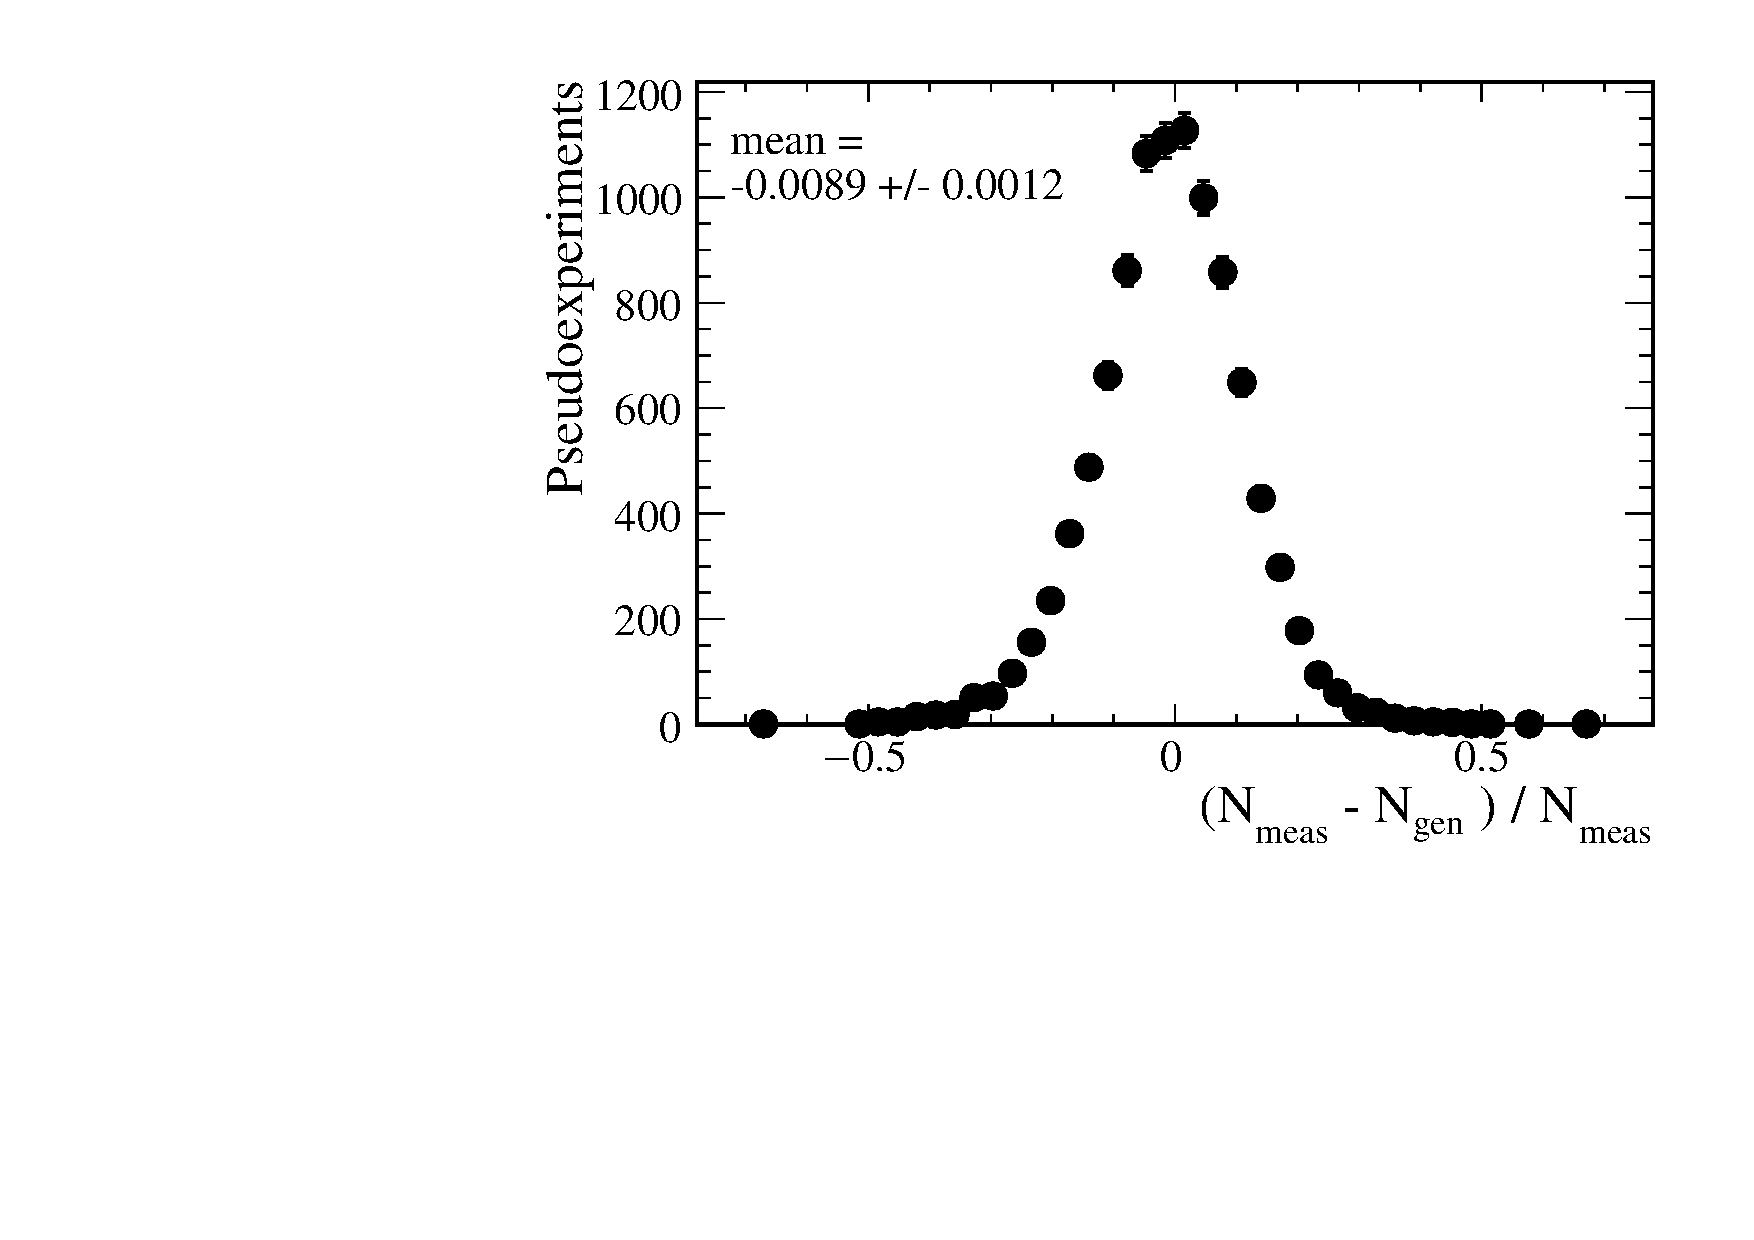
\includegraphics[width=0.6 \textwidth]{./Figs/LifetimeSystematics/Fractional_bias_Bsmumu_yield_CKM.pdf}
    \caption{Fractional bias of the measured \bsmumu yield from pseudoexperiments for the expected number of decays with 4.4 \fb. Only \bsmumu and combinatorial background decays are included in the pseudoexperiments.}
    \label{fig:FracBias}
\end{figure}


Furthermore, the pull distributions for \bsmumu yields for pseudoexperiments with higher statistics produce means that tend towards 0 as the number of decays increases as shown in Figure~\ref{fig:BsmumuYieldPulls} for the expected number of decays with 50 and 300 \fb. Therefore the mass fit returns accurate yields for \bsmumu and the biased pull distribution arises from the low statistics of the data set. The same reasoning can be applied to the pull distribution of the yields of combinatorial background decays that have a sightly less bias mean value of $\sim0.006$ compared to the \bsmumu yields.

\begin{figure}[htbp]
    \centering
        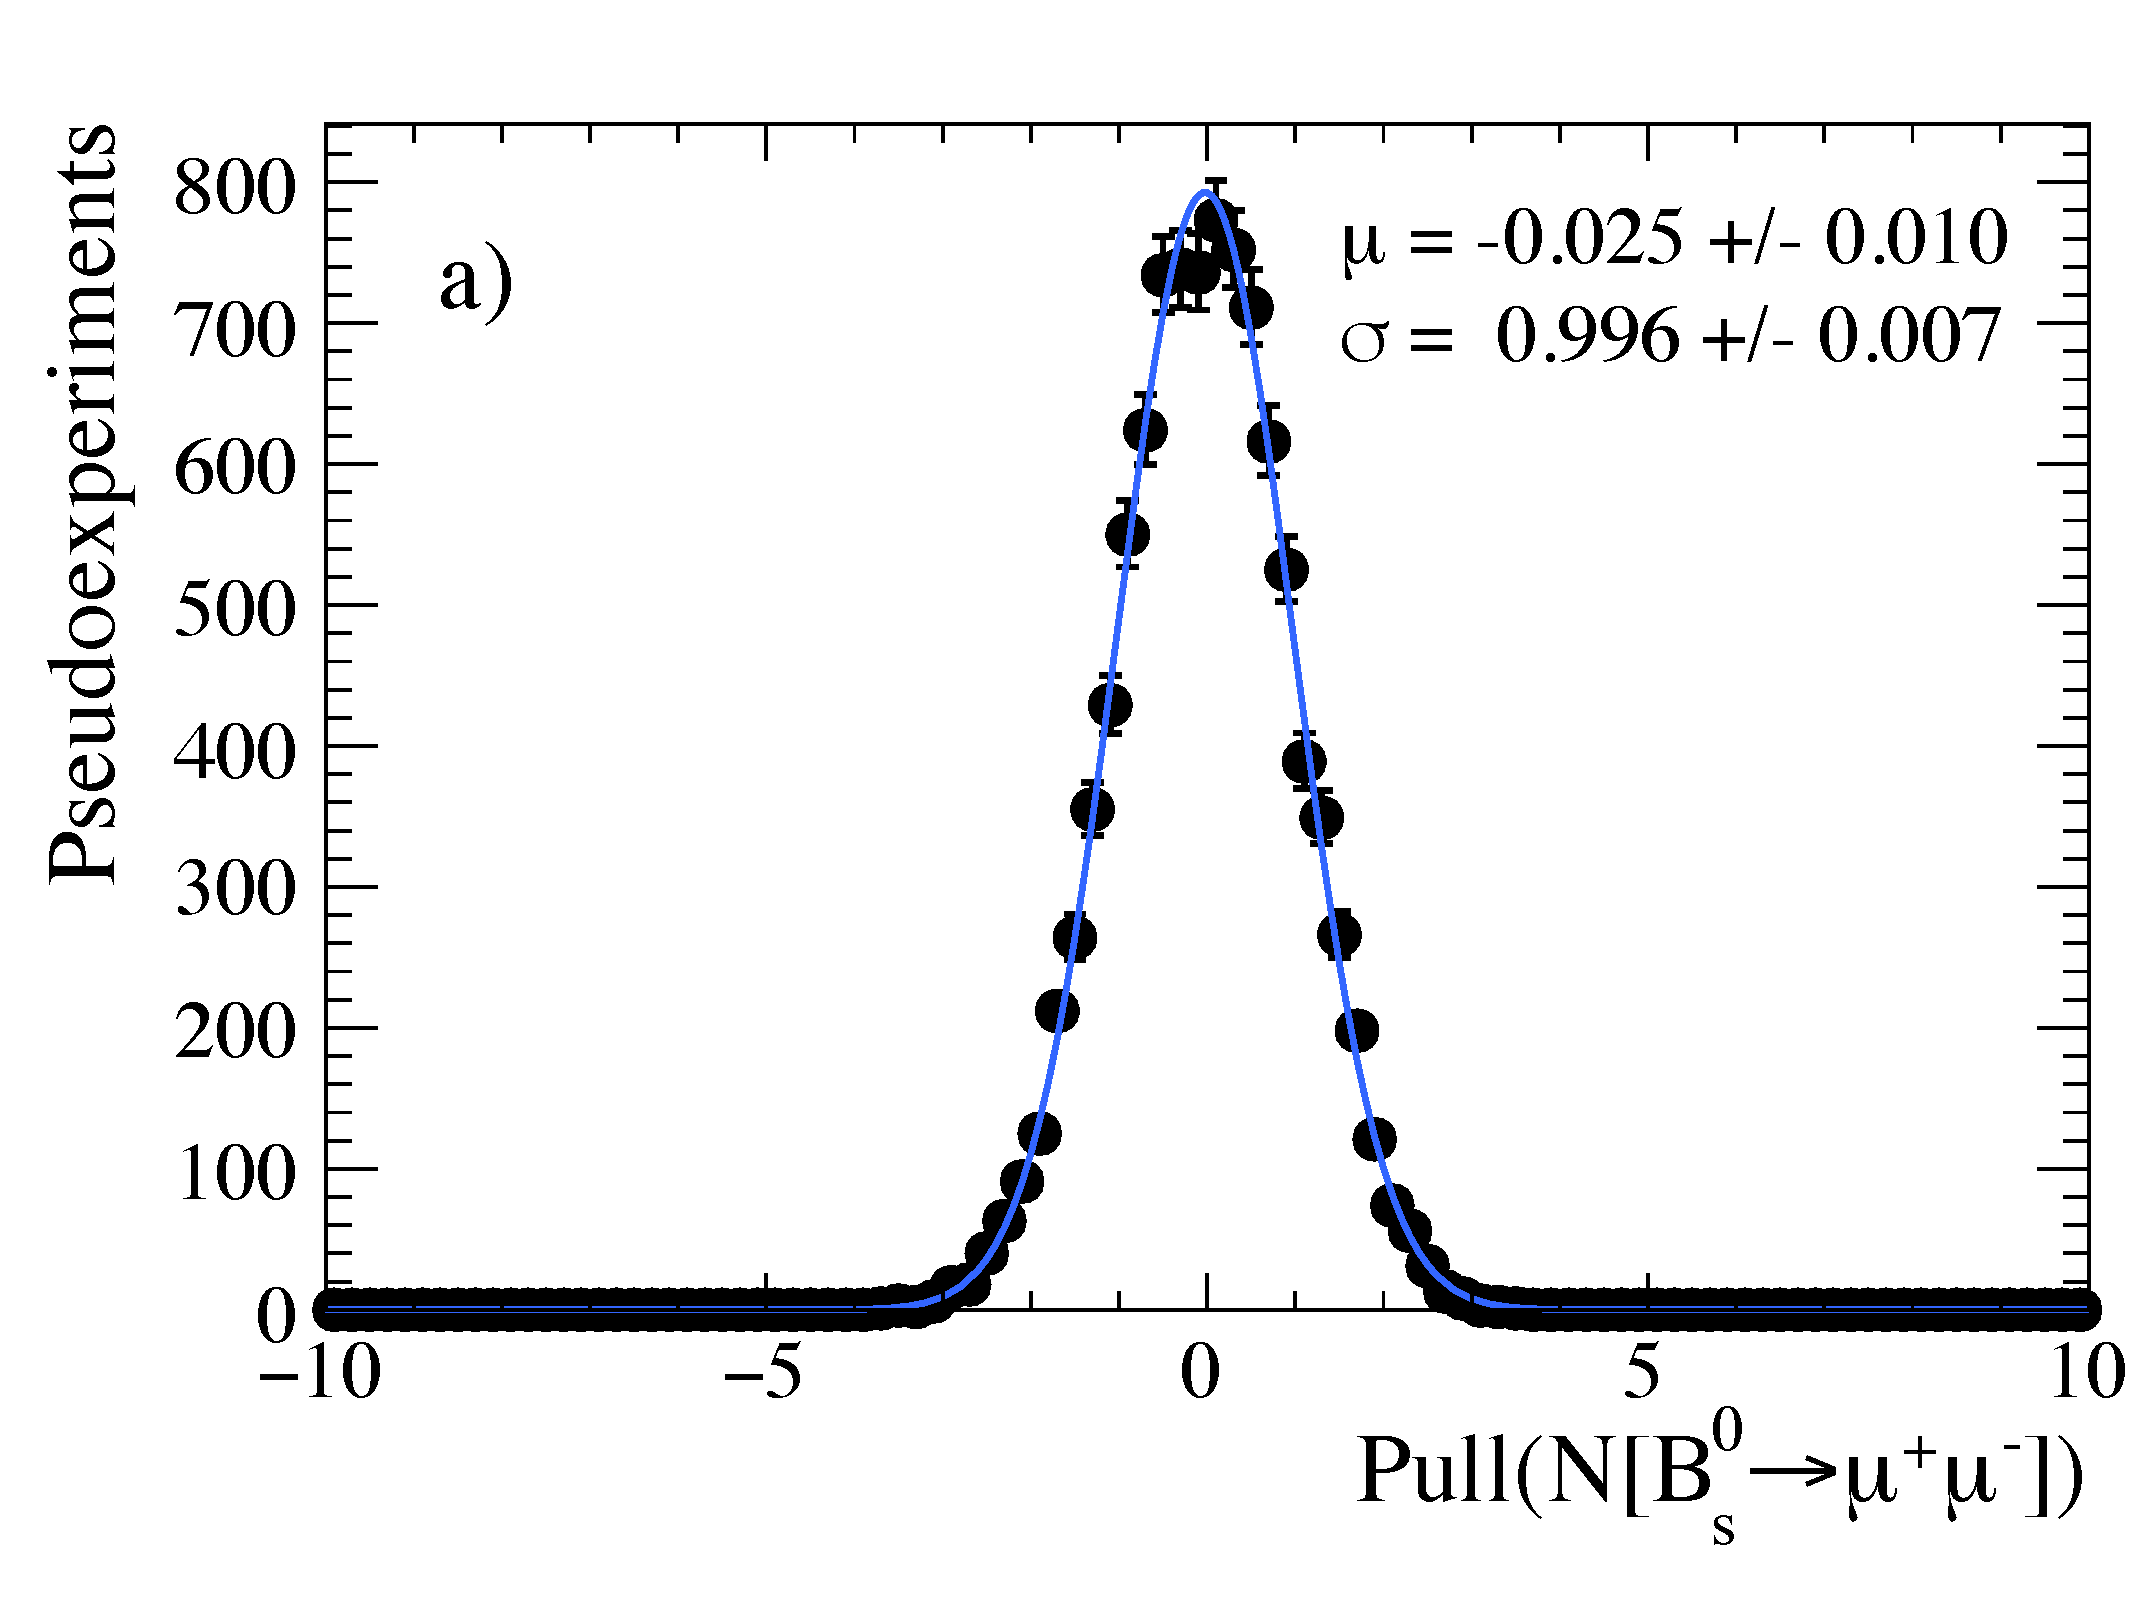
\includegraphics[width=0.49 \textwidth]{./Figs/LifetimeSystematics/Bs2MuMu_yield_pull_50fb.pdf}
        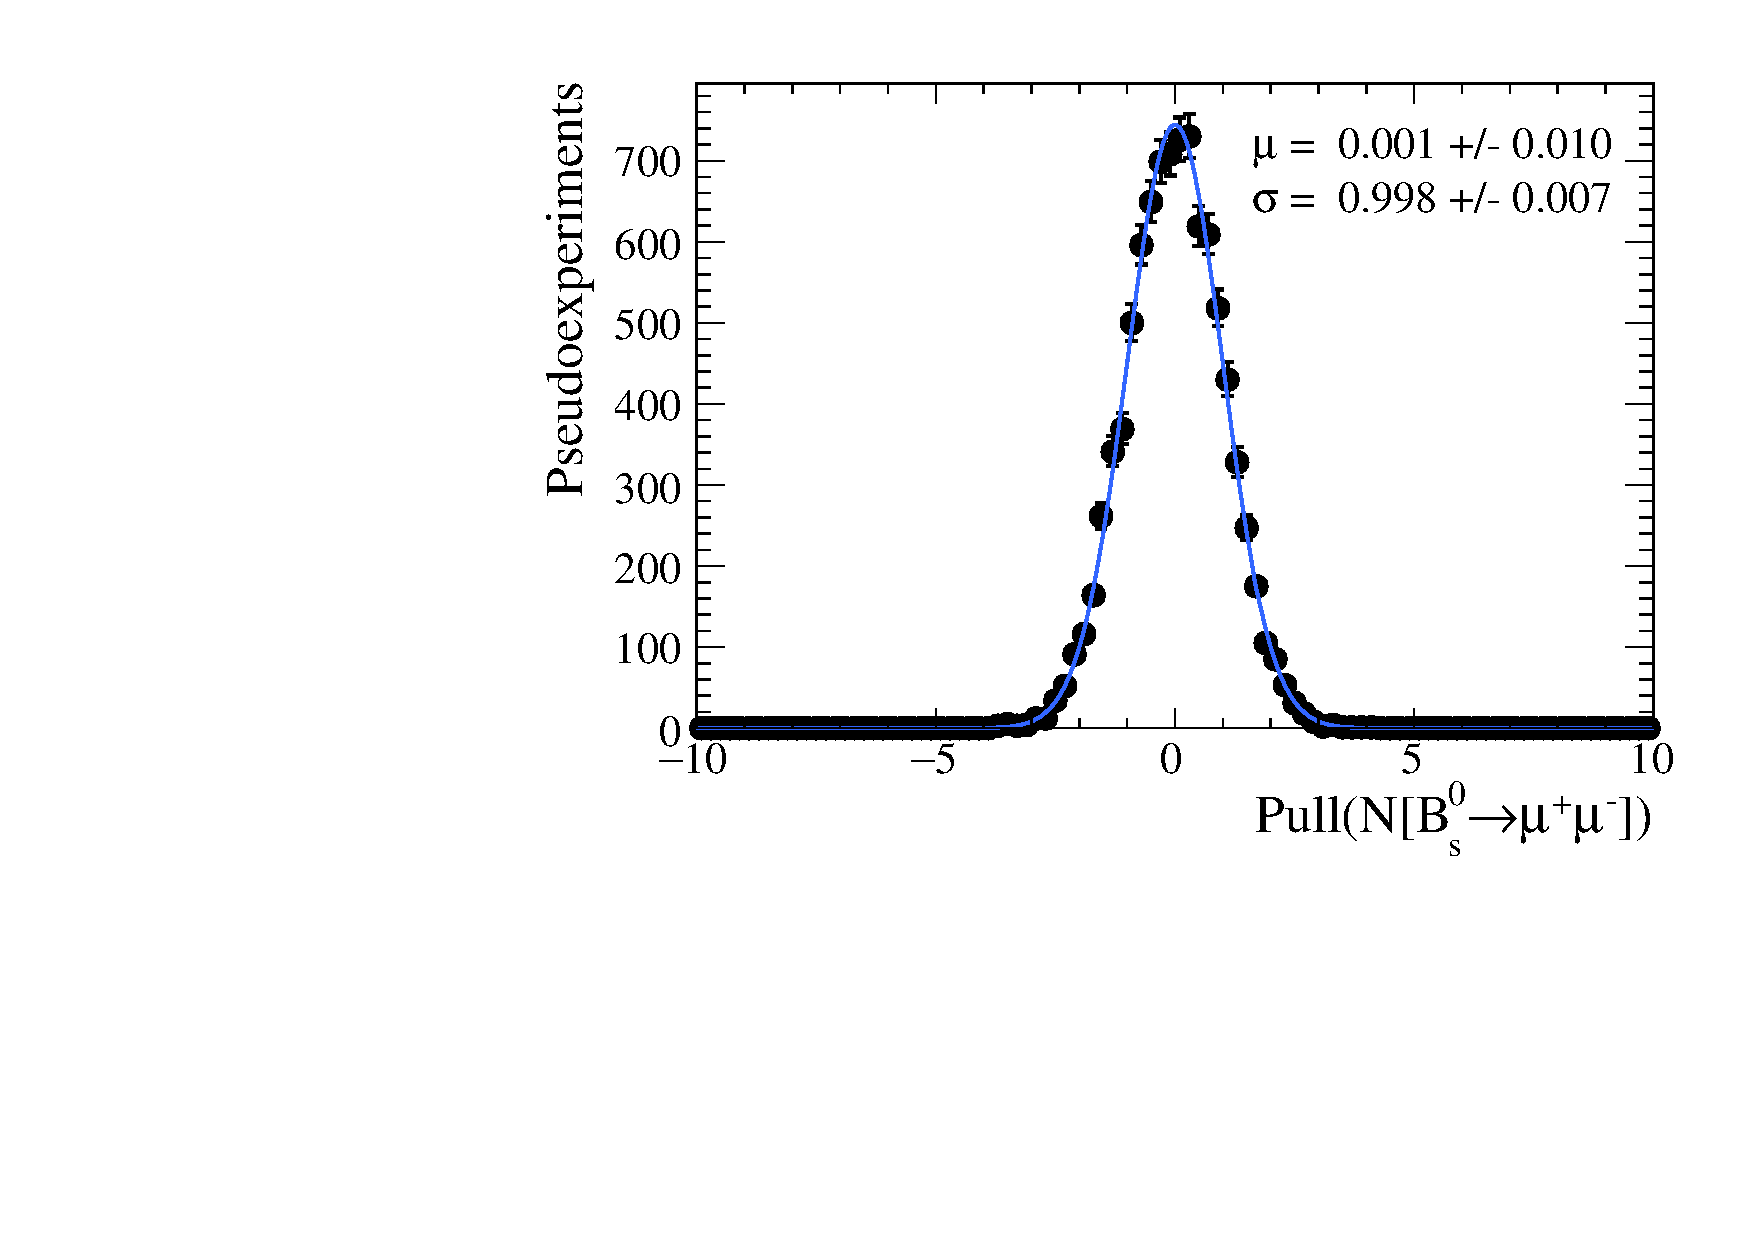
\includegraphics[width=0.49 \textwidth]{./Figs/LifetimeSystematics/Bs2MuMu_yield_pull_300fb.pdf}
    \caption{Pull distribution for \bsmumu measured yields from 10,000 pseudoexperiments for the expected number of decays in 50 and 300 \fb. Only \bsmumu and combinatorial background decays are included in the pseudoexperiments.}
    \label{fig:BsmumuYieldPulls}
\end{figure}


\subsection{Overall bias on \tmumu}
The remaining area of the fit to investigate is any underlying bias in the fit on the measured value of \tmumu. As discussed in Section~\ref{sec:tauORinvtau} the pull distribution for the measured effective lifetime is biased for the expected number of statistics but the pull distribution for \Gmumu produces a mean and width consistent with 0 and 1, respectively. However, the coverage of the uncertainties of both \tmumu and \Gmumu are reasonable and the biased \tmumu pull arises from the likelihood function as discussed in Section~\ref{sec:tauORinvtau}. 

The overall bias in the fit for measuring \tmumu is evaluated from the difference between the measured and generated values from pseudoexperiments. A total of 10,000 pseudoexperiments are performed generating only \bsmumu and combinatorial background decays. % so the fit bias is not masked by contamination from mis-identified backgrounds. 
The difference between the measured and generated \tmumu values is evaluated for pseudoexperiments with the expected and also the observed number of \bsmumu decays. The fit bias is evaluated for the observed number of decays because there are fewer than expected. The resulting distributions are shown in Figure~\ref{fig:BsmumuYieldPulls}. The mean of the difference in \tmumu values is 0.02 \ps for the expected number of decays and 0.03 \ps for the observed number of decays. Therefore the larger uncertainty of 0.03 \ps is used as the measured of the systematic uncertainty cause by the fit on the final result for \tmumu. %giving a systematic uncertainty of 0.03ps for the fit accuracy of \tmumu and no systematic uncertainty for \Gmumu.

\begin{figure}[htbp]
    \centering
        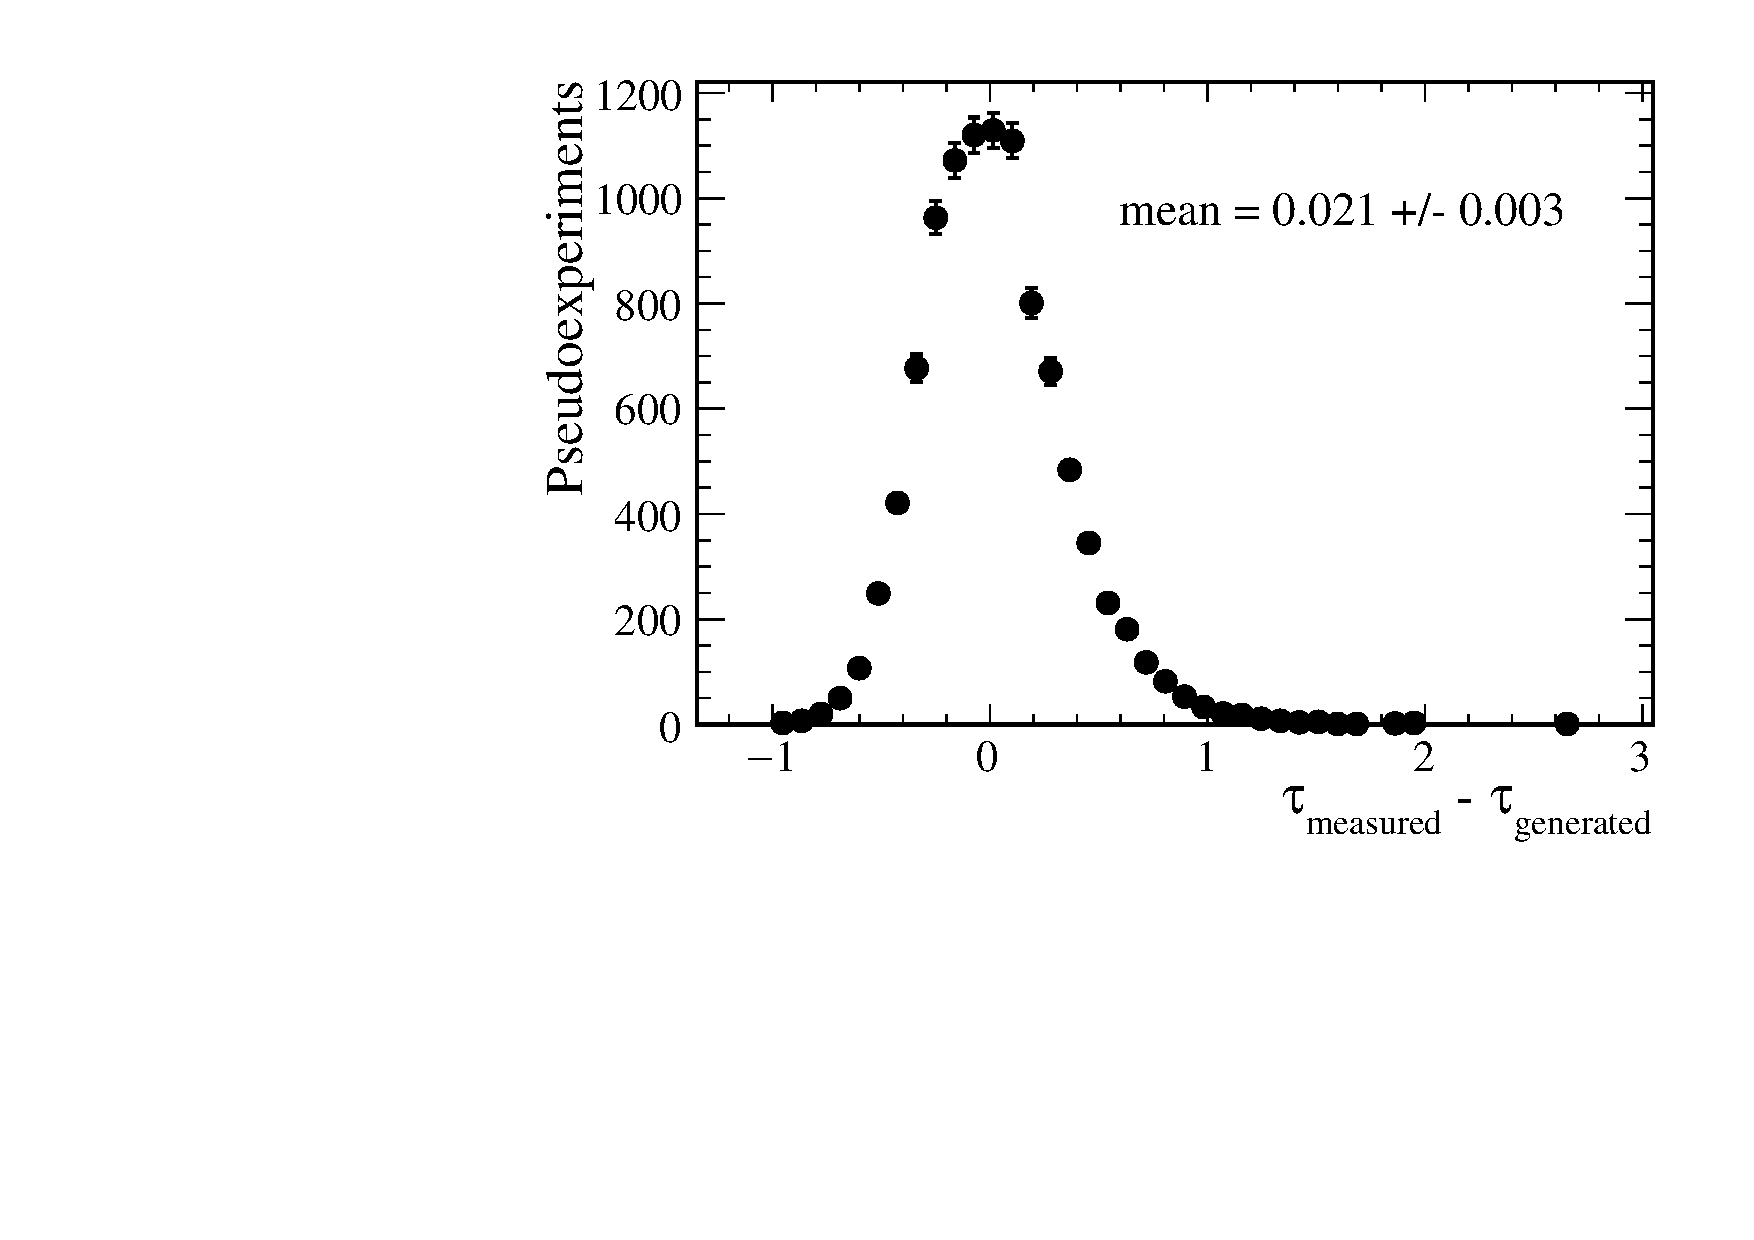
\includegraphics[width=0.49 \textwidth]{./Figs/LifetimeSystematics/tau_meas-tau_gen_expected.pdf}
        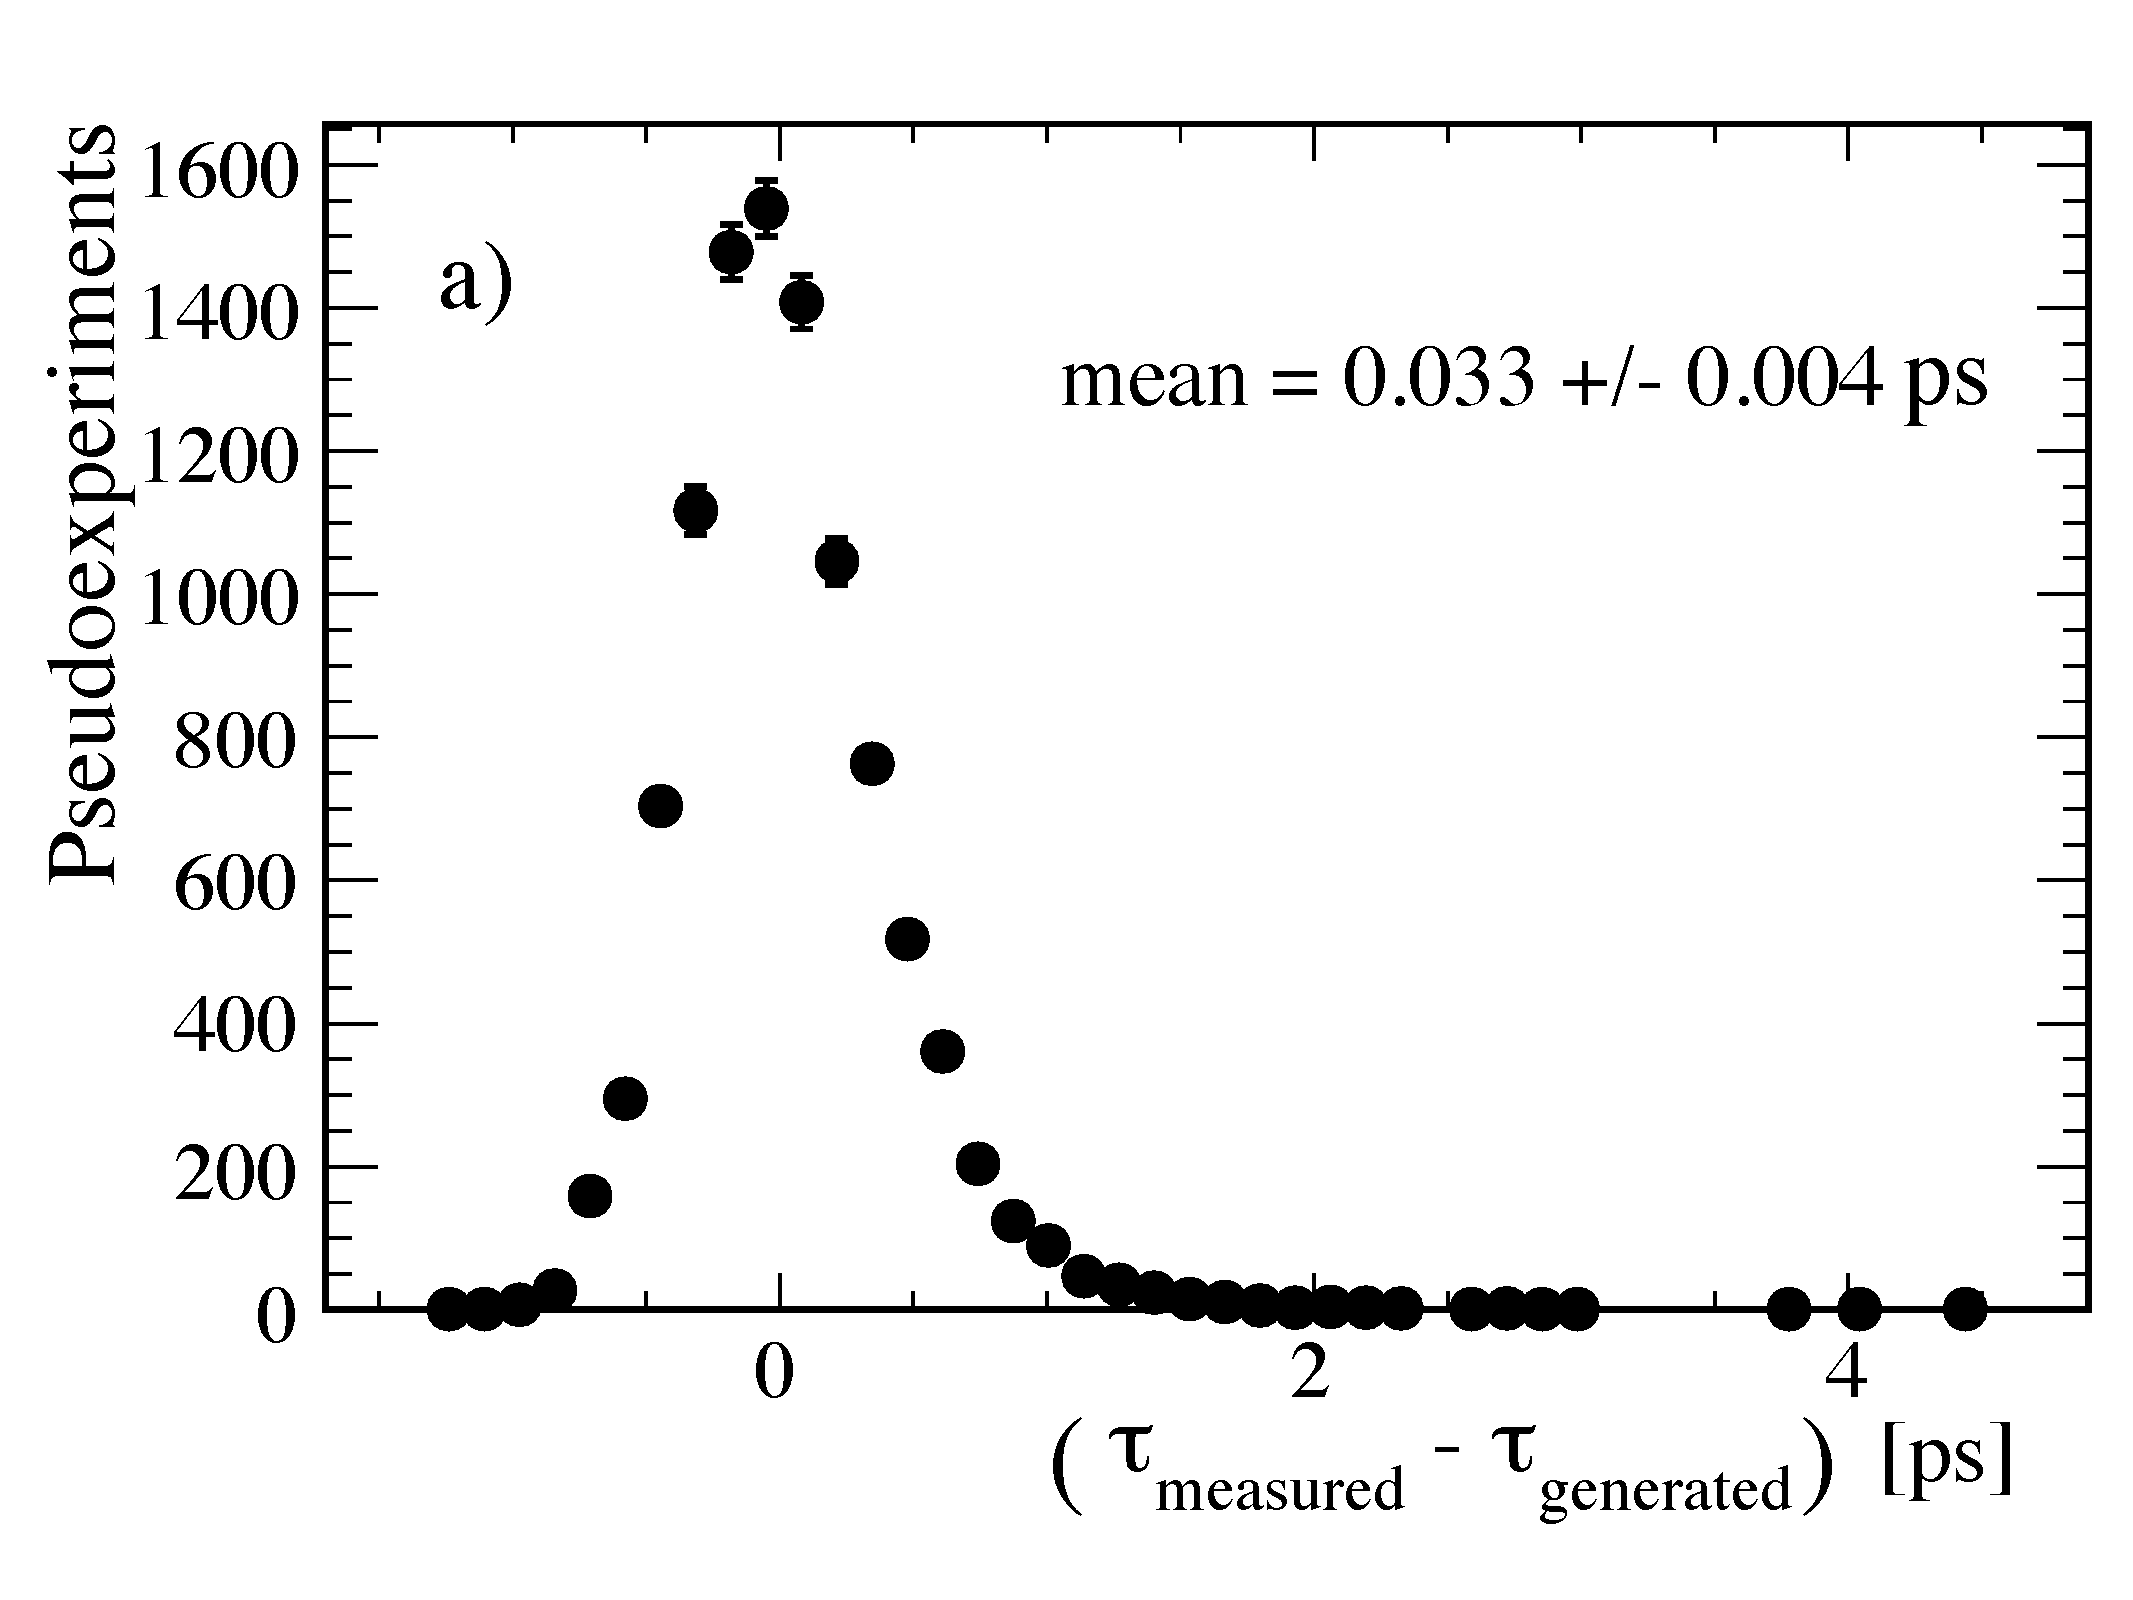
\includegraphics[width=0.49 \textwidth]{./Figs/LifetimeSystematics/tau_meas_tau_gen_observed.pdf}
    \caption{Overall bias in \tmumu, evaluated as the difference between the measured, $\tau_{measured}$, and the generated, $\tau_{generated}$, lifetimes for pseudoexperiments using the expected (left) and observed (right) \bsmumu and combinatorial background yields.}
    \label{fig:BsmumuYieldPulls}
\end{figure}


\section{Background contamination}
\label{sec:BKGcontaim}
The mass fit configuration used to measure the \bsmumu effective lifetime includes components for \bsmumu and combinatorial background decays and candidates with a \bs mass between 5320 - 6000 \mevcc. Although the majority of background decays from mis-identified decays and \bdmumu decays fall outside this mass window, as shown in Figure~\ref{fig:toygen}, the tails of some backgrounds still need to be accounted for. The backgrounds of particular importance for the chosen mass range include \bdmumu, \bhh, \lambdab, \bdpimunu, \bsKmunu, \bupimumu, \bdpimumu, \bcjpsimunu, with \bhh, \bdmumu and \lambdab being of particular importance for the chosen mass range. 

The number of expected background decays and their mass \pdfs in the range 4900 - 6000 \mevcc were computed using the methods described in Chapter~\ref{sec:BFanalysis} and the number of decays expected in the smaller mass range 5320 - 6000 \mevcc are computed by integrating the mass \pdfs. The expected yields for each background are given in Table~\ref{tab:tabC} and are less than 1 candidate, except the combinatorial background, in the range 5320 - 6000 \mevcc.  
\begin{table}[htbp]
\begin{center}
\begin{tabular}{lcc}
\toprule \toprule
Decay & \multicolumn{2}{c}{Expected yields in mass ranges} \\ 
 & 4900 - 6000 \mevcc & 5320 - 6000 \mevcc \\ \midrule
\bsmumu & 30.9 & 30.5 \\ 
\bdmumu & 3.3& 0.2\\ 
\bhh & 9.7& 0.9\\ 
\lambdab &  13.3 & 0.6\\ 
\bdpimunu & 40.5 & 0.1 \\ 
\bsKmunu &  9.1 & 0.0\\ 
\bupimumu &  6.0 & 0.0\\ 
\bdpimumu  &  4.9 & 0.6\\ 
\bcjpsimunu  &  9.8 & 0.0\\ 
Combinatorial background & 66.2 & 40.6\\ 
\bottomrule \bottomrule
\end{tabular}
\vspace{0.7cm}                                                                                                                                               
\caption{Number of expected signal and background decays in data passing the \bsmumu effective lifetime selection in the mass ranges 4900 - 6000 \mevcc and 5320 - 6000 \mevcc.}
\label{tab:tabC}
\end{center}
\vspace{-1.0cm}                                                                                                                                               
\end{table}

The impact of backgrounds not modelled in the mass fit on the measured \tmumu value is evaluated using two sets of pseudoexperiments. The pseudoexperiments have the same general set up as described in Section~\ref{sec:toys}. One set of pseudoexperiments assumes there are no backgrounds other than the combinatorial background and therefore only \bsmumu and combinatorial background candidates are generated. The second set of pseudoexperiments generates all possible background decays. The expected yields are fluctuated using a Poisson distribution around their expected values to two decimal places. For each configuration 10,000 pseudoexperiments are performed and the pull distributions for \Gmumu of each pseudoexperiment set up is compared. %The pull distributions for \tmumu are not used due to their non-Gaussian distribution disused in Section~\ref{sec:tauORinvtau}. 

The inclusion of all the background decays causes a shift in the mean of the \Gmumu pull distribution of 0.024 \ps$^{-1}$ as shown in Figure~\ref{fig:bkdcontam}. Therefore, assuming the expected uncertainty in Section~\ref{sec:toyresults} for \tmumu, the systematic shift from not including all backgrounds in the fit configuration is 0.007 \ps.% for \tmumu and Y for \Gmumu. 

\begin{figure}[htbp]
    \centering
        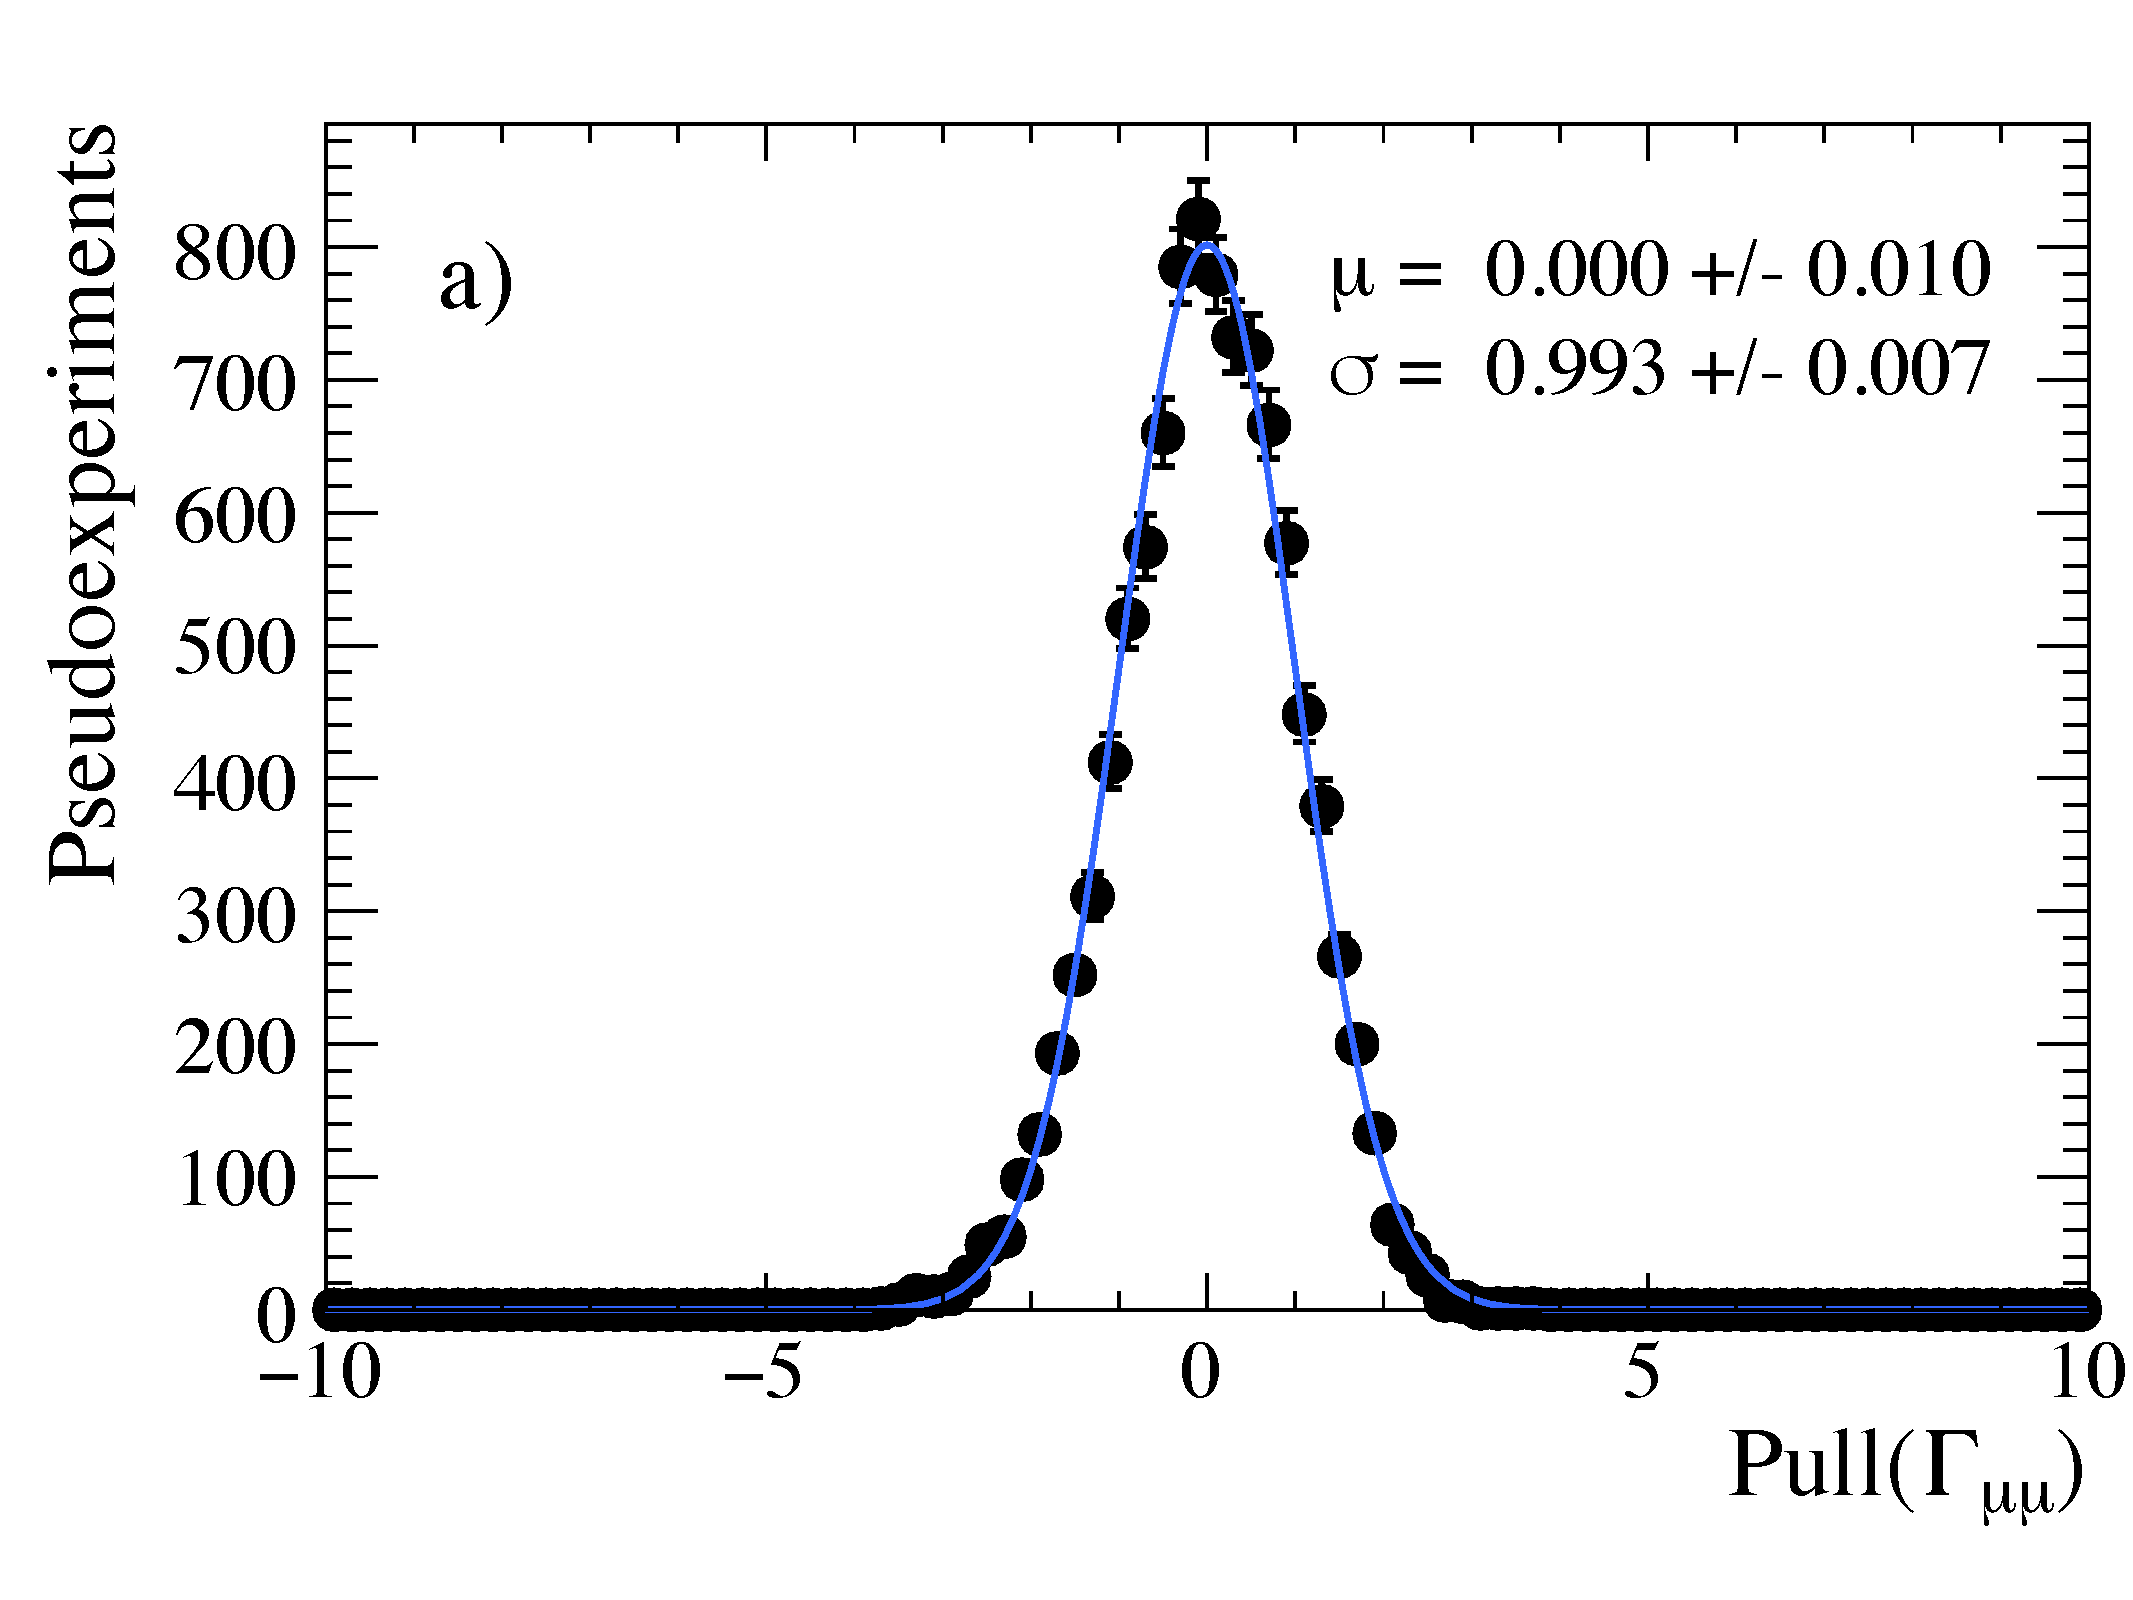
\includegraphics[width=0.49 \textwidth]{./Figs/LifetimeSystematics/Gamma_pull_mass_pdf_Run1.pdf}
        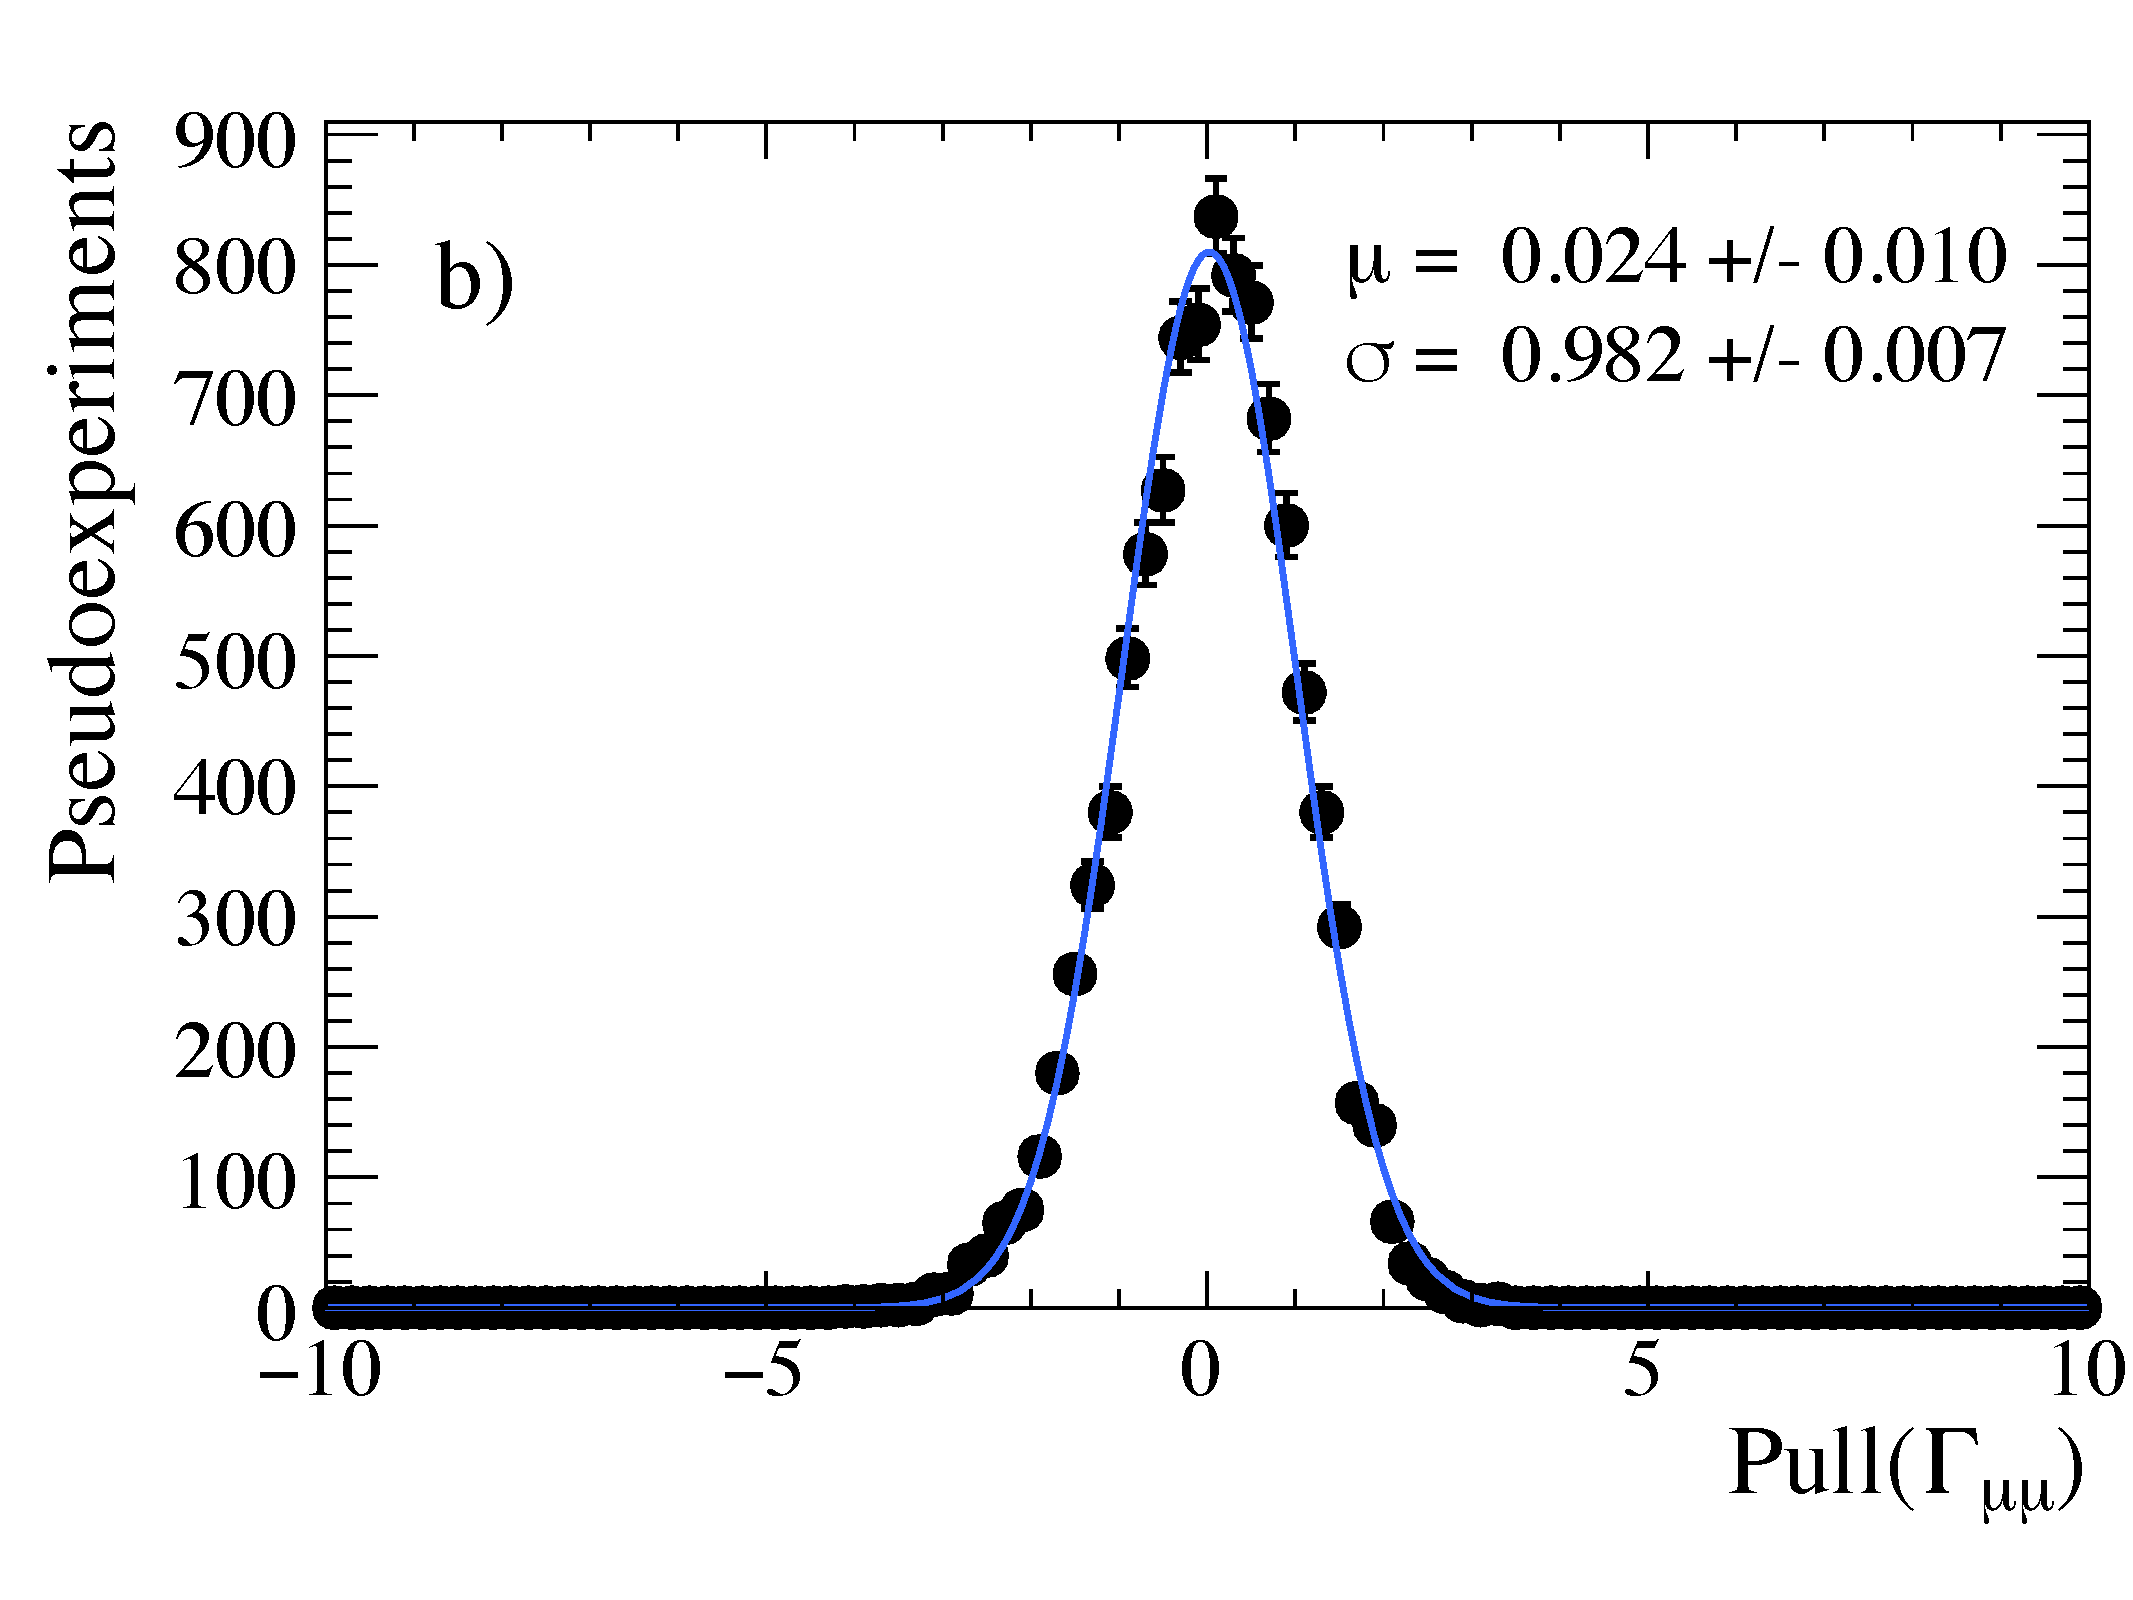
\includegraphics[width=0.49 \textwidth]{./Figs/LifetimeSystematics/5320_all_bkgnds_gamma_pull_CKM.pdf}
    \caption{Pull distribution for \Gmumu from 10,000 pseudoexperiments, using background sources of combinatorial background only (left) and combinatorial background, mis-identified decays and \bdmumu decays (right).}
    \label{fig:bkdcontam}
\end{figure}

The expected number of \bsmumu and \bdmumu decays assumes the SM branching fractions. However, the measured values for the \BFs are slightly different from the SM predictions, excluding the results presented in Chapter~\ref{sec:BFanalysis}. Using the measured values from the combined analysis of the Run~1 CMS and LHCb data~\cite{CMS:2014xfa}, the expected number of \bsmumu and \bdmumu decays decreases and increases, respectively, compared to the SM expectations. The changes in the yields are given in Table~\ref{tab:tabD}. The pseudoexperiments were repeated with the world average \BFs but the shift in the mean of the pull distribution was smaller, therefore the larger value from the SM predictions are used.
\begin{table}[htbp]
\begin{center}
\begin{tabular}{lcc}
\toprule \toprule
Decay & \multicolumn{2}{c}{Expected yield in 5320 - 6000 \mevcc} \\ 
 & Standard Model & World average \\ \midrule
\bsmumu & 30.5 & 22.5 \\ 
\bdmumu & 0.2& 0.7\\ 
\bottomrule \bottomrule
\end{tabular}
\vspace{0.7cm}                                                                                                                                               
\caption{Number of expected decays in data passing the \bsmumu effective lifetime selection in the mass range 5320 - 6000 \mevcc using the Standard Model predictions and branching fraction measurements from the combined analysis of the Run~1 CMS and LHCb data~\cite{CMS:2014xfa}.}
\label{tab:tabD}
\end{center}
\vspace{-1.0cm}                                                                                                                                               
\end{table}

\section{Mass \pdf parameters}
\label{sec:massPDFsyst}
The data collected in Run~1 and Run~2 are combined for the measurement of the \bsmumu effective lifetime and the mass and decay time fits are applied to the combined data. However the parameters used in the mass \pdf in Table~\ref{tab:signalpdfRun1} were evaluated specifically for Run~1 data and different parameters are available for Run~2 data. Therefore, the influence of the choice of mass \pdf parameters on the measured \tmumu value must be evaluated. 

Once again pseudoexperiments are performed to understand the size of the impact of the mass model choice on the effective lifetime measurement. Only \bsmumu and combinatorial background decays are generated to separate mass \pdf effects from the contamination of mis-identified backgrounds and \bdmumu decays in the mass window. \bsmumu candidates are generated using the Run~1 parameters in Table~\ref{tab:signalpdfRun1} but the mass fit is performed using the Run~2 parameters in Table~\ref{tab:signalpdfRun2}. The pull distribution for 10,000 pseudoexperiments for \Gmumu from this configuration are compared with those from pseudoexperiments where Run~1 parameters are used to generate and fit the mass distribution. The change in the measured lifetime with the mass \pdf parameters is negligible as shown in Figure~\ref{fig:masspdfsyst}. Therefore, no systematic uncertainty is assigned. 

\begin{figure}[htbp]
    \centering
        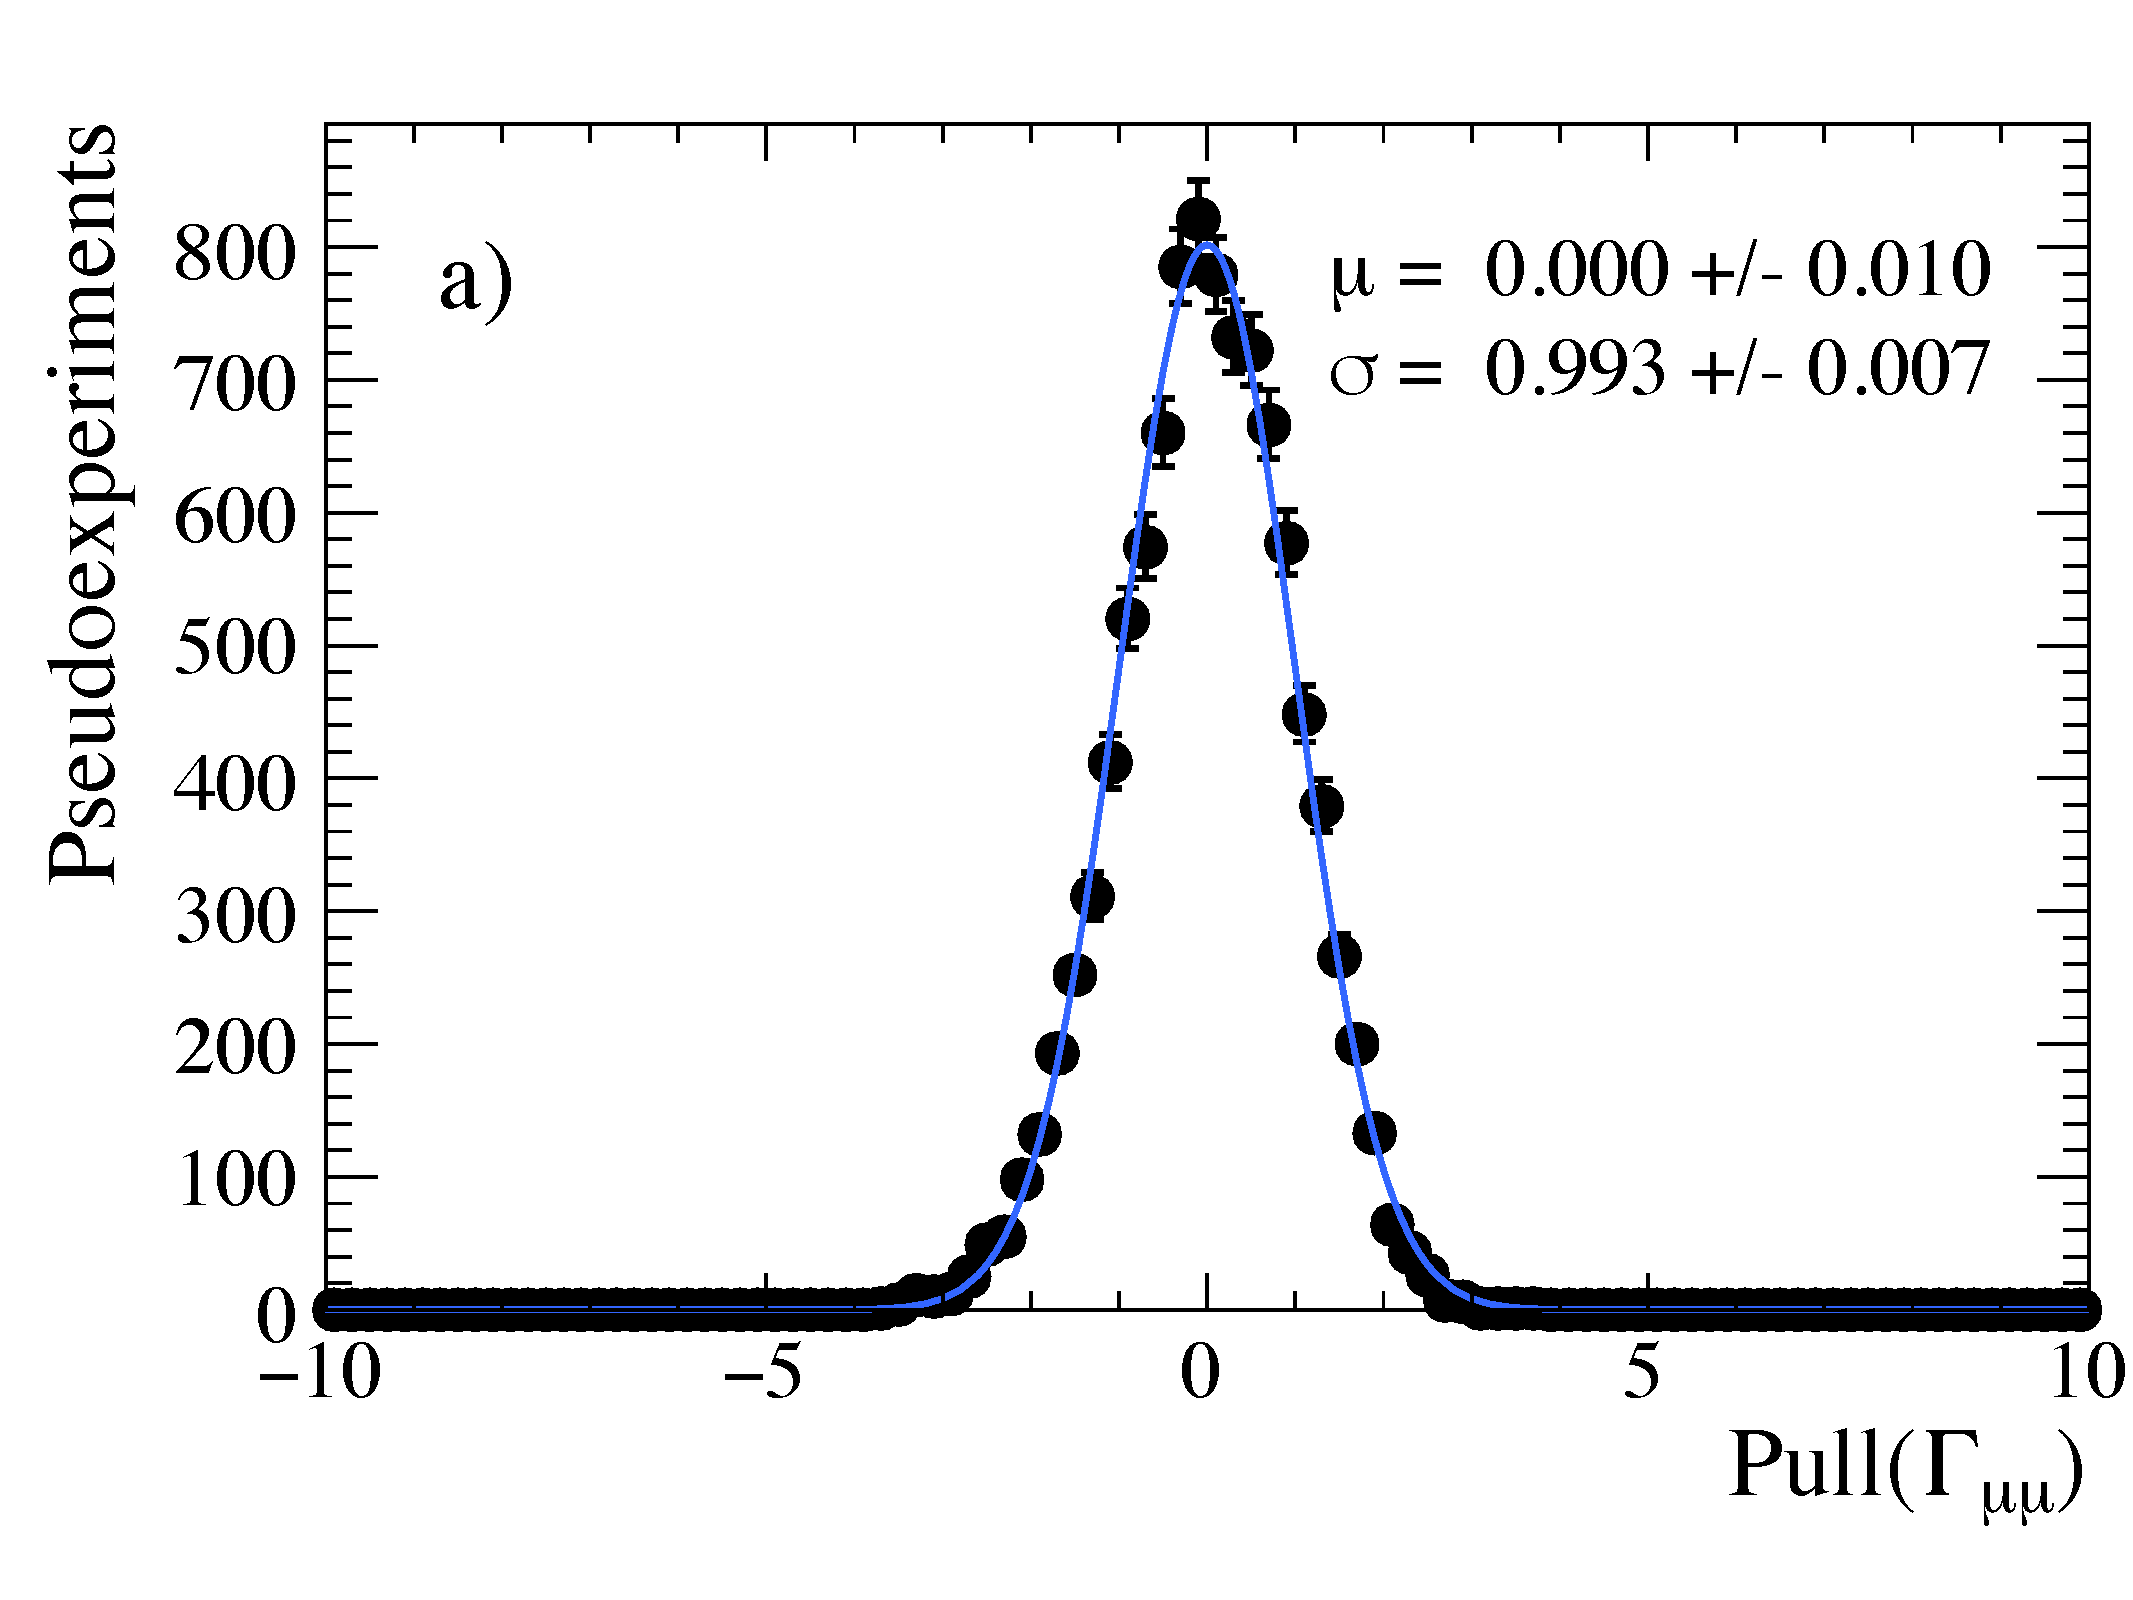
\includegraphics[width=0.49 \textwidth]{./Figs/LifetimeSystematics/Gamma_pull_mass_pdf_Run1.pdf}
        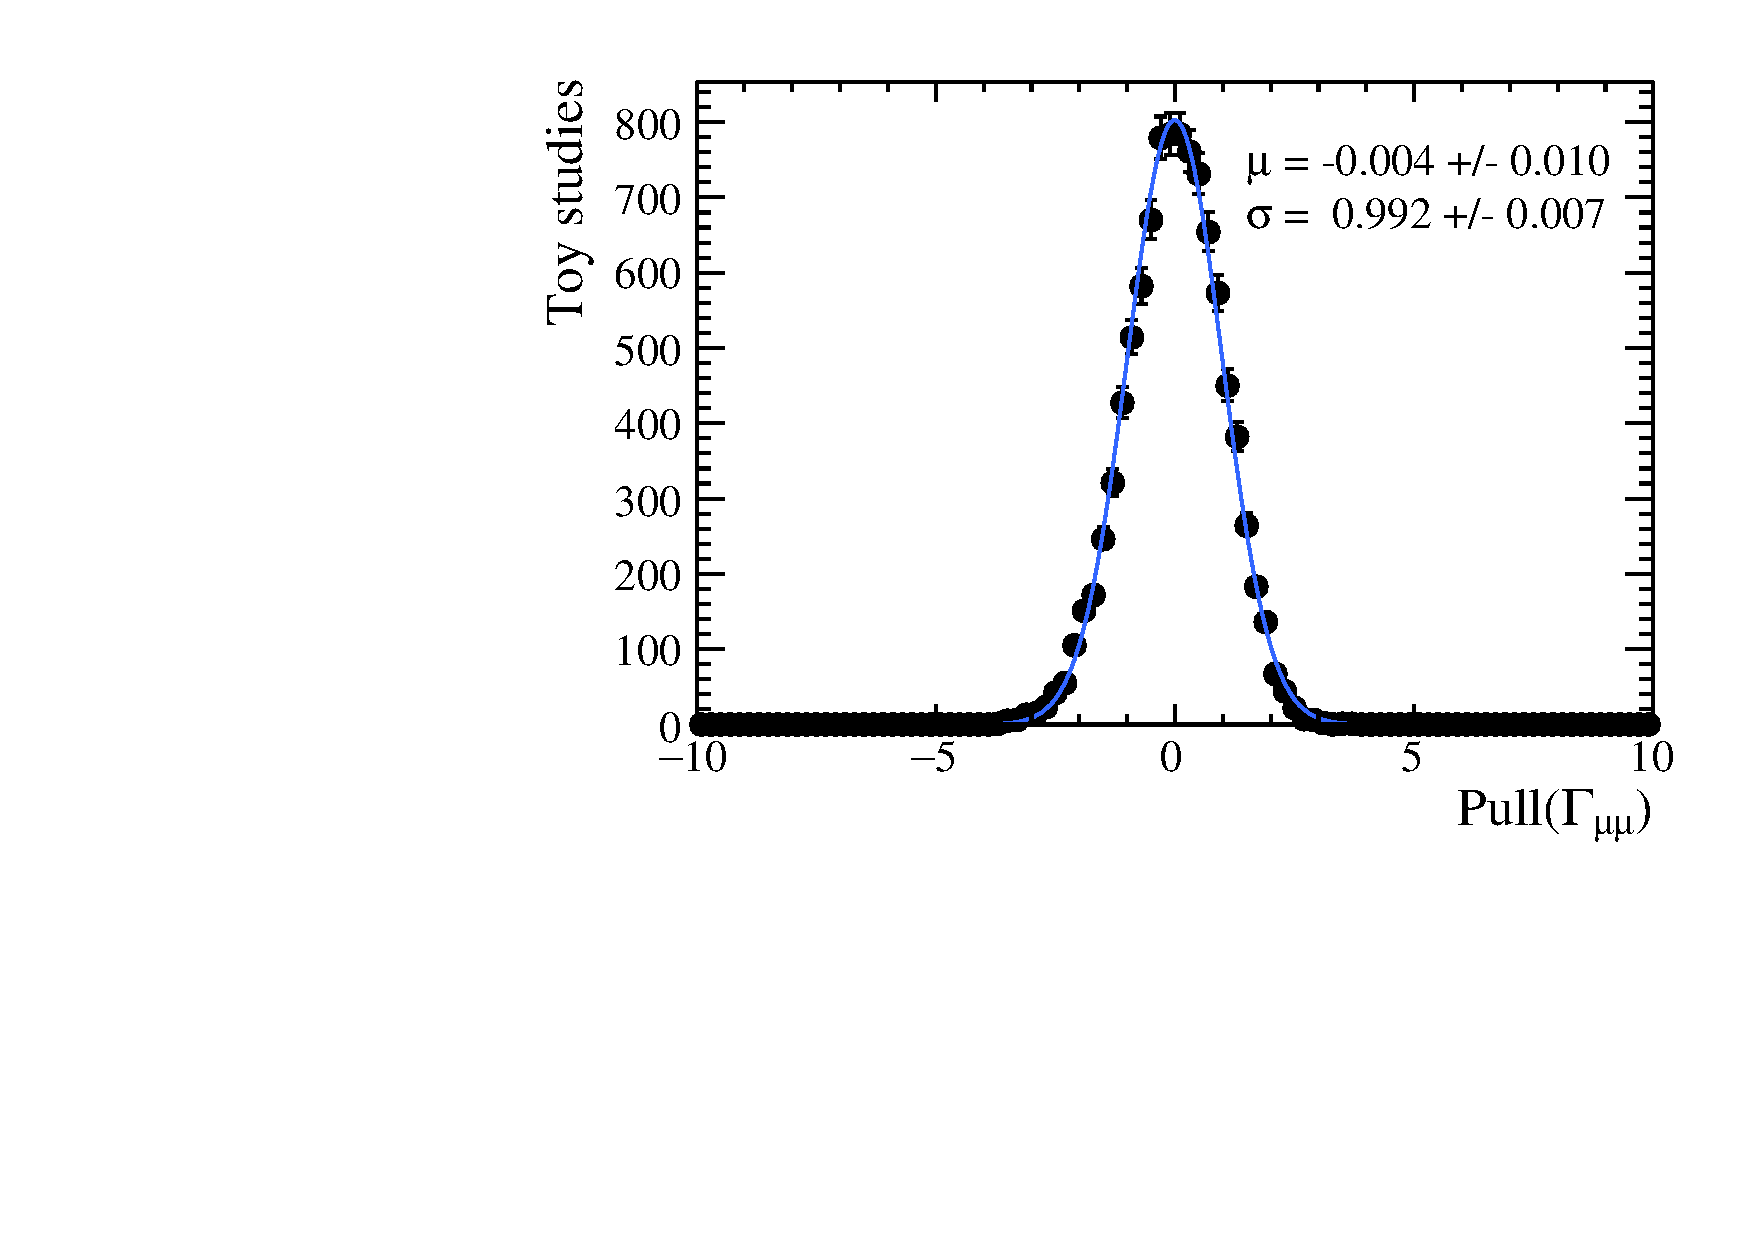
\includegraphics[width=0.49 \textwidth]{./Figs/LifetimeSystematics/Gamma_pull_mass_pdf_Run2.pdf}
    \caption{Pull distribution for \Gmumu from 10,000 pseudoexperiments where the \bsmumu mass distribution is generated using the Run~1 parameters and the mass fit is performed using Run~1 parameters (left) and Run~2 parameters (right).}
    \label{fig:masspdfsyst}
\end{figure}


\section{Acceptance function accuracy}
\label{sec:accptsyst}
The decay time acceptance function is determined from weighted simulated decays, as described in Section~\ref{sec:signalDTpdf}. It relies on the assumption that weighted simulated decays model the data reasonably well. To test this assumption, as well as the strategy used to measure the \bsmumu effective lifetime, the lifetimes of the more abundant \bdkpi and \bskk decays are measured using the same approach as the \bsmumu lifetime.

%\bdkpi decays have a much larger branching fraction the \bsmumu decays at XXX and are therefore more abundant in data. 
The selection requirements used to identify \bdkpi decays in 2011, 2012, 2015 and 2016 data are detailed in Chapter~\ref{selection_chapter} and are kept very similar to the \bsmumu selection. Although considerably reducing the statistics, all candidates are required to be triggered as TIS, in order to keep the \bhh trigger efficiency similar to that of \bsmumu decays. %\bhh triggers are $\%$ efficient, 
The trigger lines that identify \bsmumu decays in data are relatively unbiased with respect to the \bs decay time distribution. The same is true for trigger lines that identify \bhh decays as TIS, whereas TOS triggers that identify \bhh decays create a large bias of the decay time distribution due to the dependence on the trigger lines on \bs IP, IP \chisqd and flight distance.
% the TIS triggers are relatively unbiased with respect to the decay time similarly to triggers that select \bsmumu decays. Whereas TOS triggers that identify \bhh decays create a large bias on the decay time distribution due to the dependence on the trigger lines on IP, IP \chisqd and flight distance variables. 
The DLL$_{K\pi}$ variable is used to separate \bdkpi decays from other \bhh decays and candidates are reconstructed with the daughter with the highest DLL$_{K\pi}$ value assigned the kaon mass hypothesis and the daughter particle with the lowest DLL$_{K\pi}$ value the pion mass hypothesis.

The measurement of the \bdki lifetime is performed in the same way as the \bsmumu effective lifetime measurement and all years of data are combined into one data set. An extended unbinned maximum likelihood fit is performed to the \bdkpi mass distribution. Components for \bdkpi, \bskpi and combinatorial background decays are included in the mass fit. Both B meson decays are modelled by Crystal Ball functions and combinatorial background decays are modelled by an exponential function. The mass fit, shown in Figure~\ref{fig:bdkpimassfit}, is used to calculate sWeights that are re-normalised using Equation~\ref{eq:sWeightsrex}. The lifetime, $\tau_{K\pi}$, is  measured from the sWeighted decay time distribution. 

\begin{figure}[htbp]
\centering
  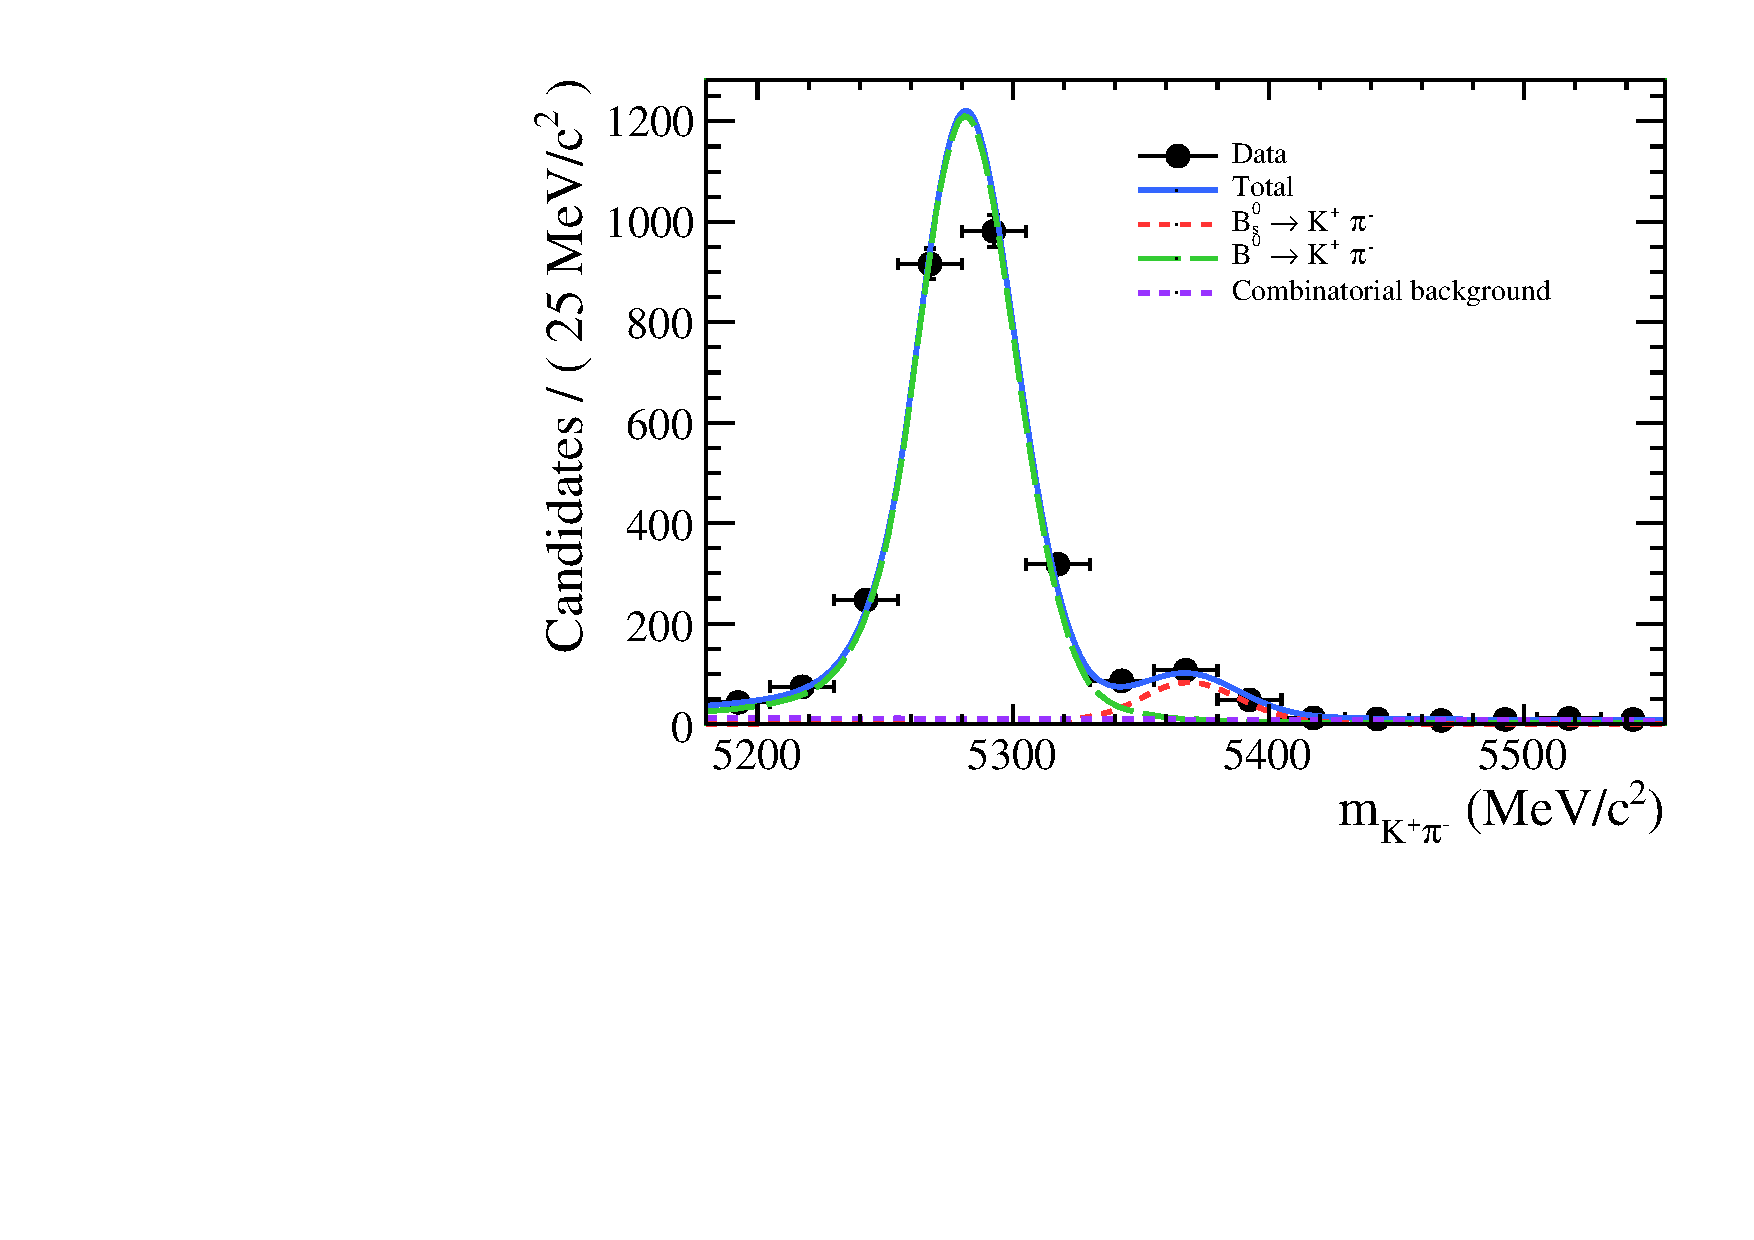
\includegraphics[width=0.6\textwidth]{./Figs/LifetimeSystematics/Bd2KPi_mass_fit.pdf}
\caption{Maximum likelihood fit to the mass distribution of \bdkpi decays for data taken in 2011, 2012, 2015 and 2016. Components for \bdkpi, \bskpi and combinatorial background decays are included. }
\label{fig:bdkpimassfit}
\end{figure}


The decay time \pdf has the same form as the one used for the \bsmumu decays in Equation~\ref{eq:DTpdf}. The acceptance parameters are found from a fit to weighted \bdkpi simulated decays using the same method described in Section~\ref{sec:signalDTpdf} with the number of tracks in the event are weighted using the same weights as \bsmumu decays. However, the weights applied to combine simulated \bdkpi decays from each year are not dependant on \bsjpsiphi decays. Since \bdkpi decays have a high yield in data, mass fits to each year are used to find the yields and combine the simulated decays from each year. The same mass \pdf used to fit the combined mass distribution is applied to each year. The weights used to combine simulated decays in different years are
\begin{equation}
\omega_{i}  = \frac{Y_{i}^{data}}{\displaystyle\sum_{j} Y_{j}^{data}} \cdot \frac{\displaystyle\sum_{k} N_{k}^{K\pi}}{N_{i}^{K\pi}},
\end{equation}
where $Y_{i}^{data}$ are the \bdkpi yields in each year of data and $N_{i}^{K\pi}$ the number of simulated decays available for each year.
The acceptance function fit is shown in Figure~\ref{fig:bdkpiacceptancefit} and for consistency the same simulation versions are used for \bdkpi decays as \bsmumu decays. 

\begin{figure}[htbp]
\centering
  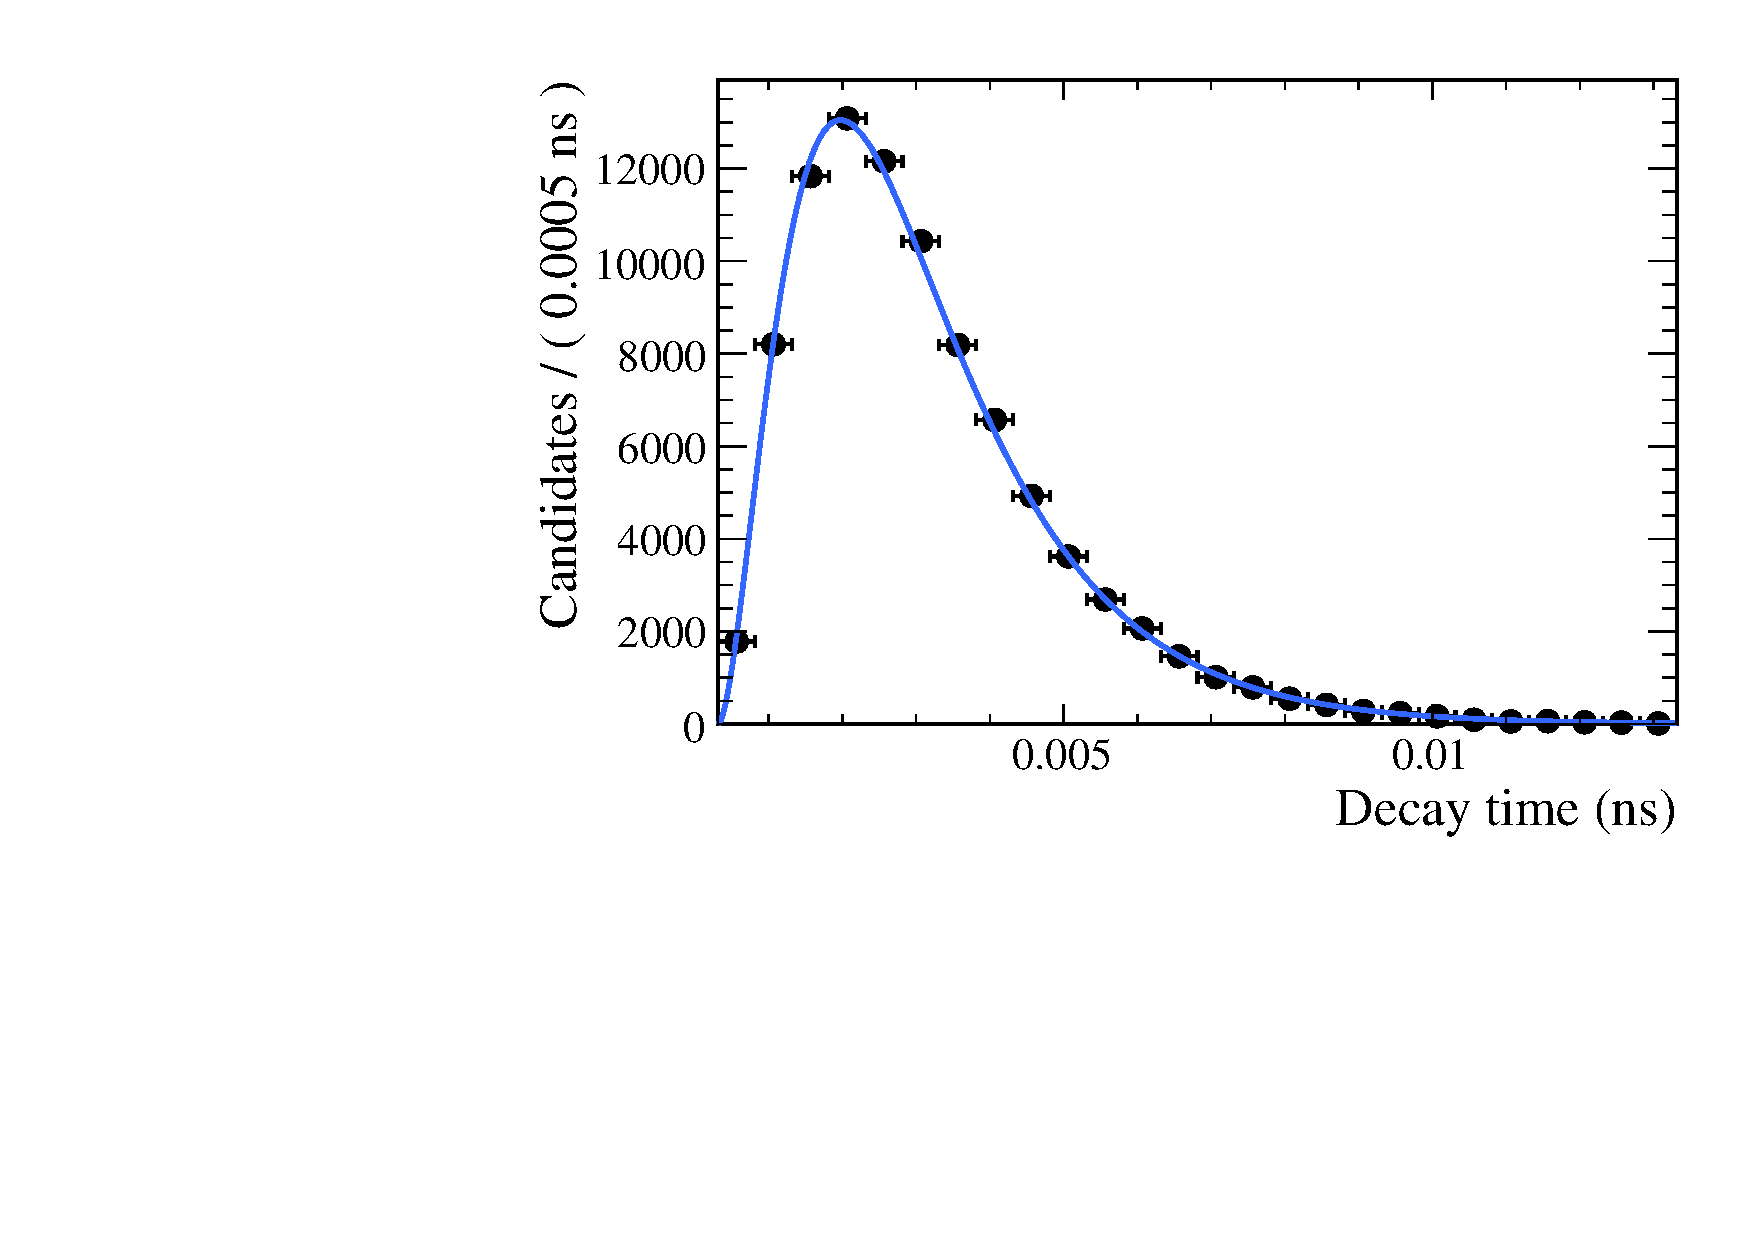
\includegraphics[width=0.6\textwidth]{./Figs/LifetimeSystematics/Bd2KPi_acceptance_fit.pdf}
\caption{Decay time distribution in weighted 2011, 2012, 2015 and 2016 simulated decays and the \ml fit results to determine the acceptance function parameters. }
\label{fig:bdkpiacceptancefit}
\end{figure}

The measured \bdkpi lifetime is
\begin{equation}
\tau_{K\pi} = 1.52 \pm 0.03  \text{ ps},
\end{equation}
%%\begin{equation}
%\Gamma_{K\pi} = XX  \pm XX \text{ ps}^{-1}
%\end{equation}
where only the statistical uncertainty is given and the decay time fit is shown in Figure~\ref{fig:bdkpilifetimefit}. The measured results are consistent with the PDF value of 1.520 $\pm$ 0.004~\ps~\cite{Olive:2016xmw} and the measurement strategy used to find the \bsmumu \el has been shown to work. The statistical uncertainty of the measured \bdkpi decay time is assigned as a systematic uncertainty to provide a measure of how well the acceptance function can be determined from weighted simulated decays for measuring \tmumu. 

\begin{figure}[htbp]
\centering
  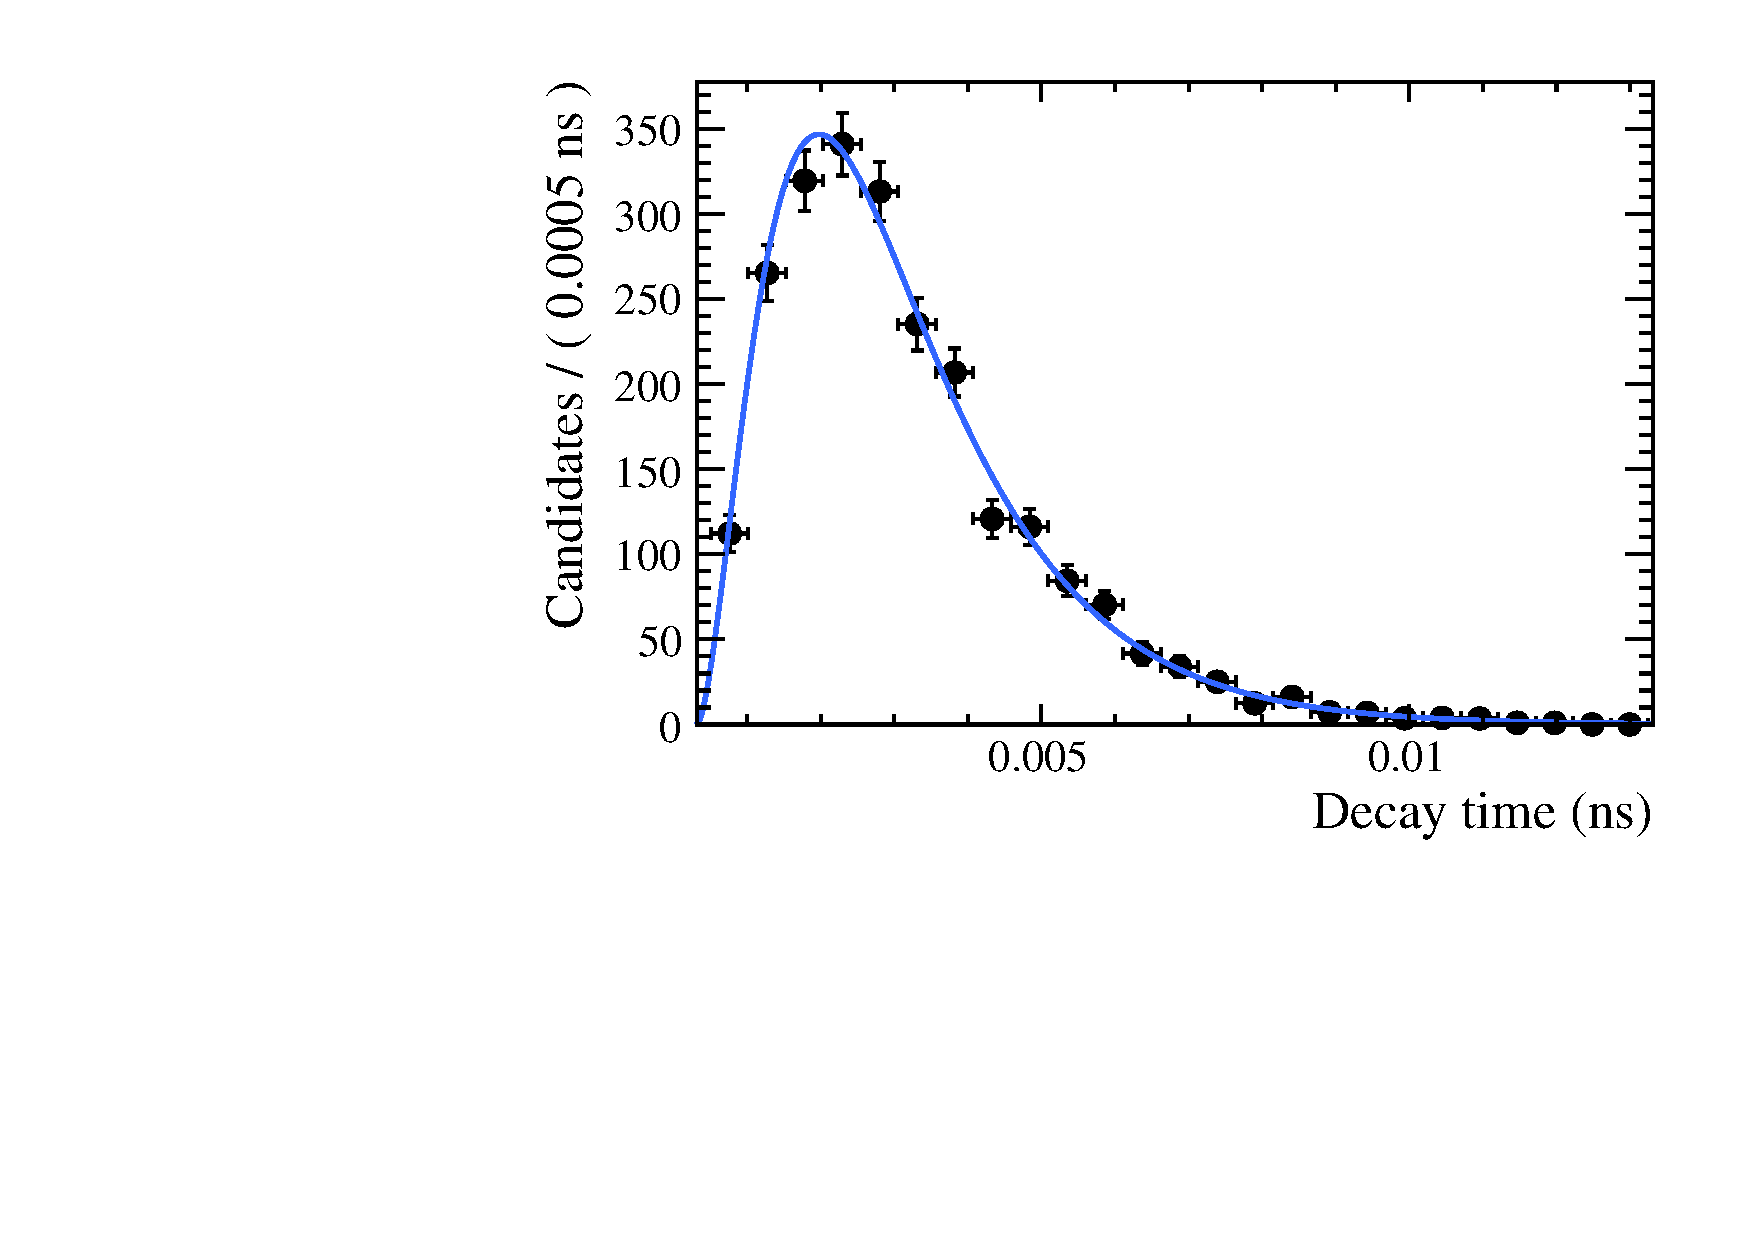
\includegraphics[width=0.6\textwidth]{./Figs/LifetimeSystematics/Bd2KPi_lifetime_fit.pdf}
\caption{Maximum likelihood fit to the signal weighted decay time distribution of \bdkpi decays for data taken in 2011, 2012, 2015 and 2016. }
\label{fig:bdkpilifetimefit}
\end{figure}

However, the determination of the \bsmumu acceptance function relies on weights taken from the number of tracks in an event for \bdkpi decays in data and simulation. Although the measurement of the \bdkpi lifetime shows the procedure and weighting method works for these decays, it does not show that the weights taken from \bdkpi decays can be applied to other decays. Therefore, as a cross check, the lifetime of \bskk decays is also measured. 

The same measurement strategy is used for \bskk decays as \bsmumu and \bdkpi and candidates in 2012 and 2015 data are identified using the selection requirements in Chapter~\ref{selection_chapter}. Only 2012 and 2015 data are used due to the available simulation versions of simulated \bskk decays compared to \bsmumu. Once again TIS triggers are used to keep a relatively lifetime unbiased trigger efficiency and candidates are reconstructed assuming both daughters are kaons. The mass \pdf includes \bskk and combinatorial background decays and the same \pdf is used for \bskk as for \bskpi. The unbinned extended \ml fit used to extract the sWeights is shown in Figure~\ref{fig:bskkmassfit}. 

\begin{figure}[htbp]
\centering
  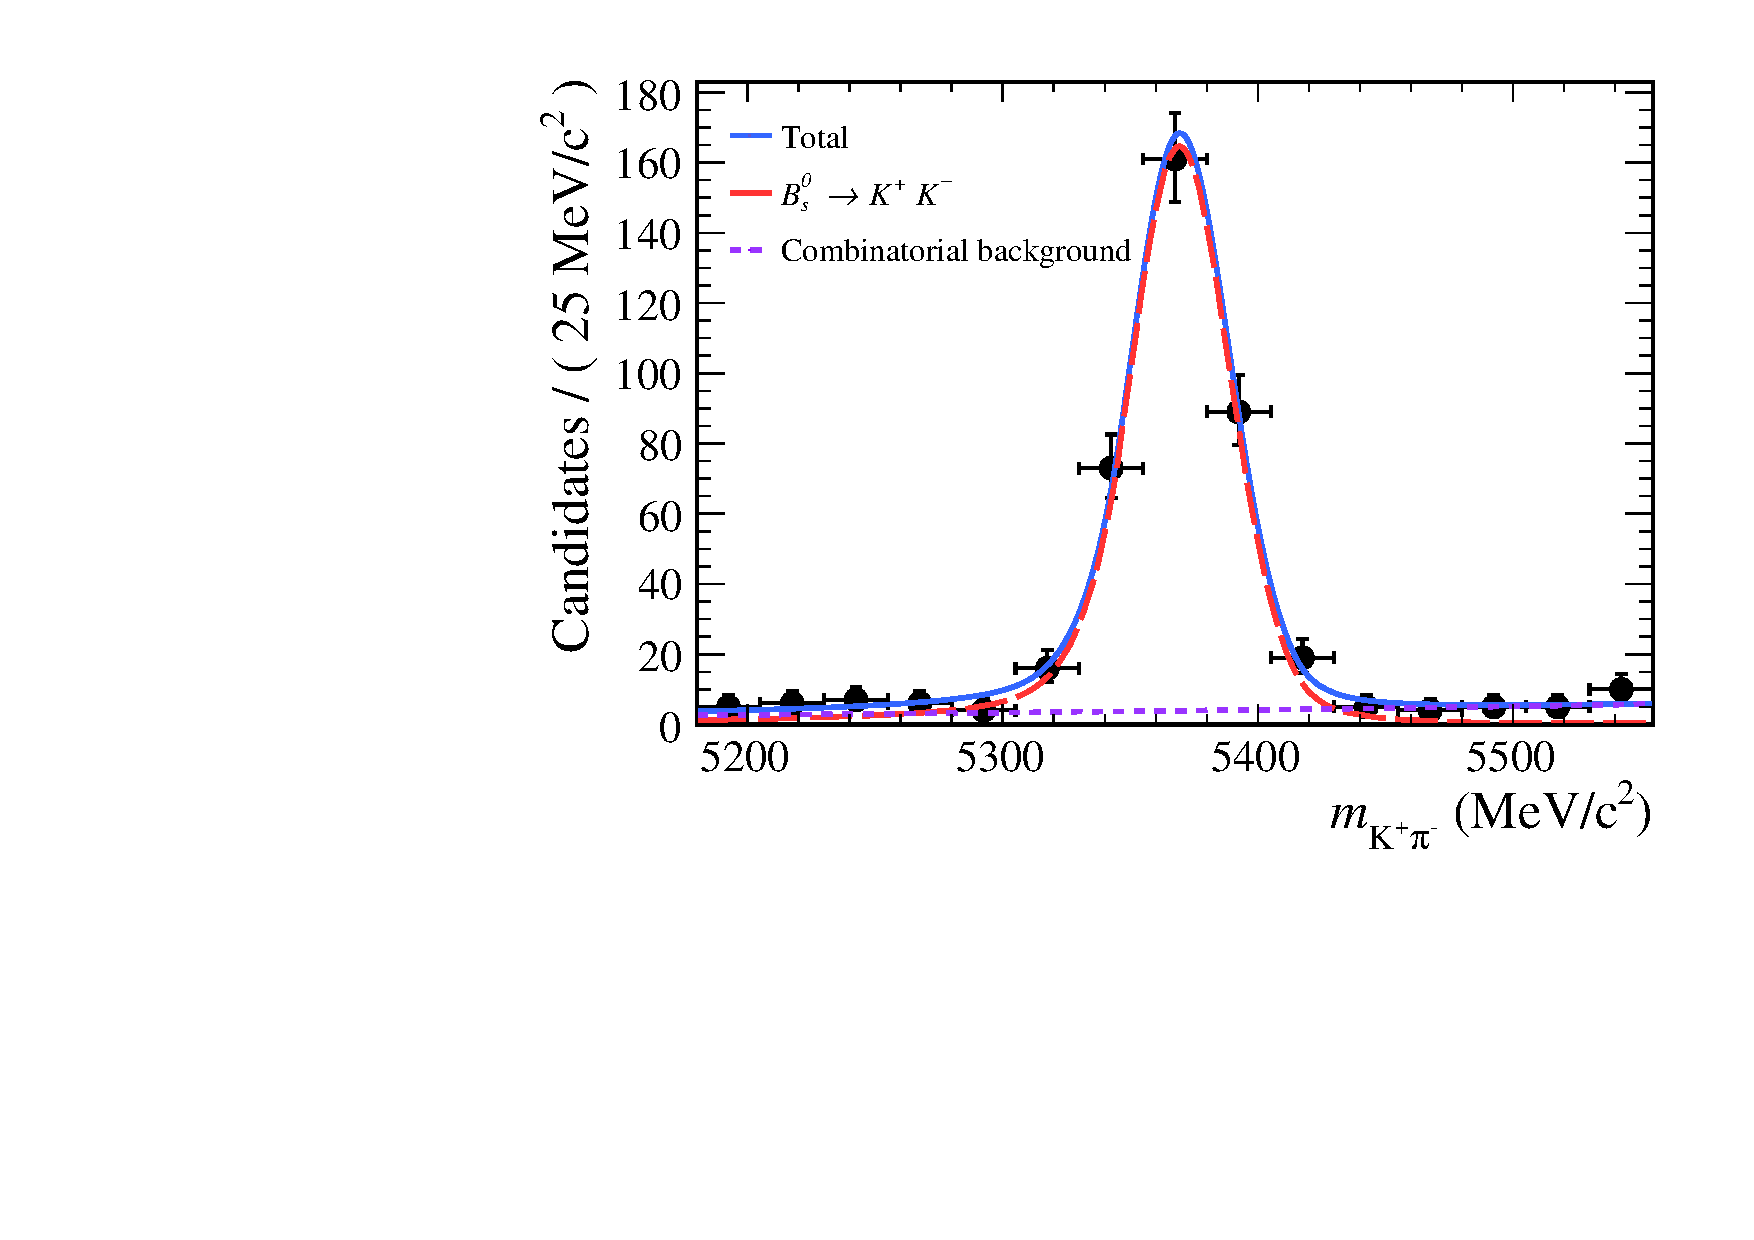
\includegraphics[width=0.6\textwidth]{./Figs/LifetimeSystematics/Bs2KK_mass_fit.pdf}
\caption{Maximum likelihood fit to the mass distribution of \bskk decays for data taken in 2012 and 2015. Components for \bskk and combinatorial background decays are included in the mass fit. }
\label{fig:bskkmassfit}
\end{figure}


The \bskk acceptance is found using the same method as \bsmumu with \bsjpsiphi decays used to determine the relative proportions of decays in each year of data. Figure~\ref{fig:bskkacceptancefit} shows the acceptance fit and the results of the decay time fit is shown in Figure~\ref{fig:bskklifetimefit}. The measured values for the lifetime, $\tau_{KK}$, is
\begin{equation}
\tau_{KK} = 1.39 \pm 0.06  \text{ ps}, 
\end{equation}
%\begin{equation}
%\Gamma_{KK} = XX  \pm XX \text{ ps}^{-1}
%\end{equation}
where only the statistical uncertainty is given.% and the fit results are shown in Figure~\ref{fig:bskklifetimefit}. 
The measured values are consistent with the predicted value of 1.395 $\pm$ 0.020 \ps \cite{Aaij:2014fia} and shows that \bdkpi weights can be used for other decays as well as \bdkpi. 

\begin{figure}[htbp]
\centering
  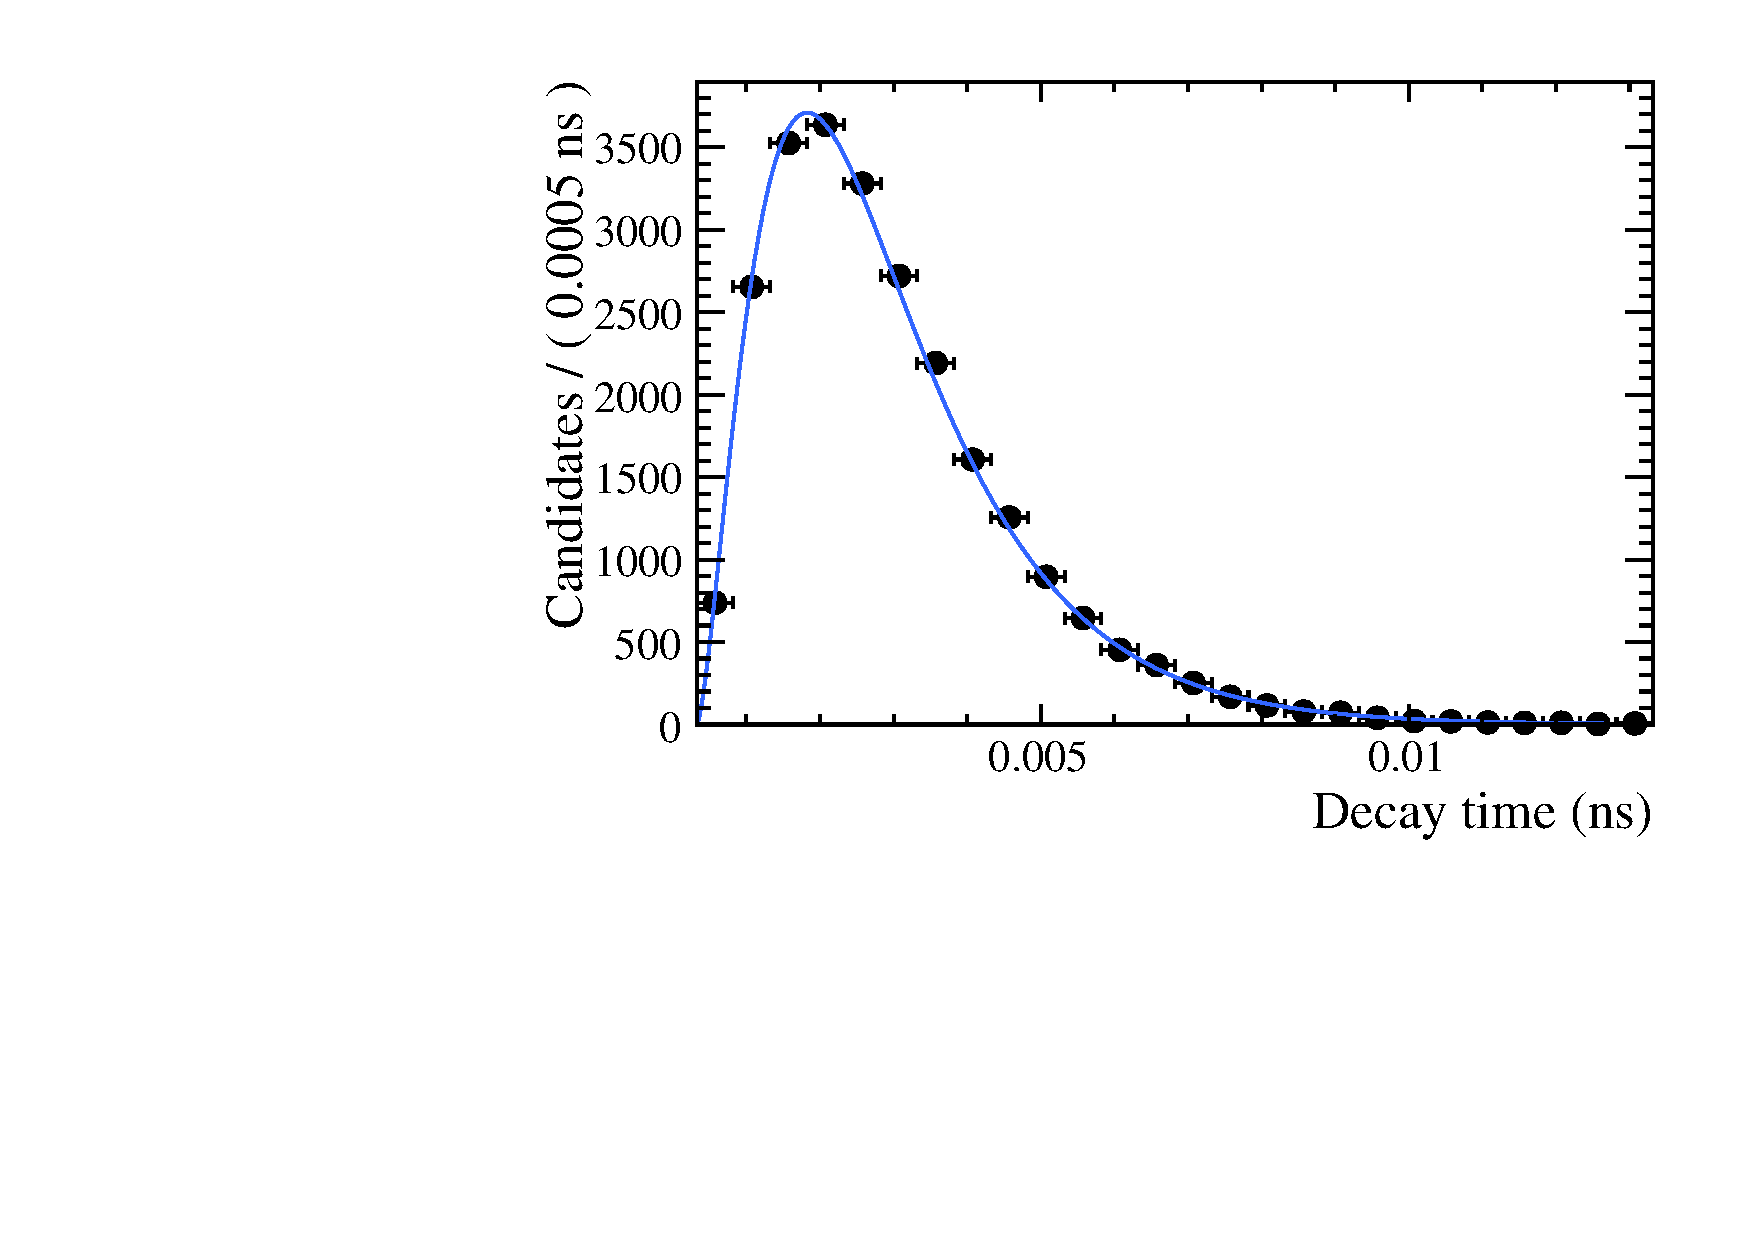
\includegraphics[width=0.6\textwidth]{./Figs/LifetimeSystematics/Bs2KK_acceptance_Fit.pdf}
\caption{Decay time distribution in weighted 2012 and 2015 simulated decays and the fit  results to determine the acceptance function parameters. }
\label{fig:bskkacceptancefit}
\end{figure}

\begin{figure}[htbp]
\centering
  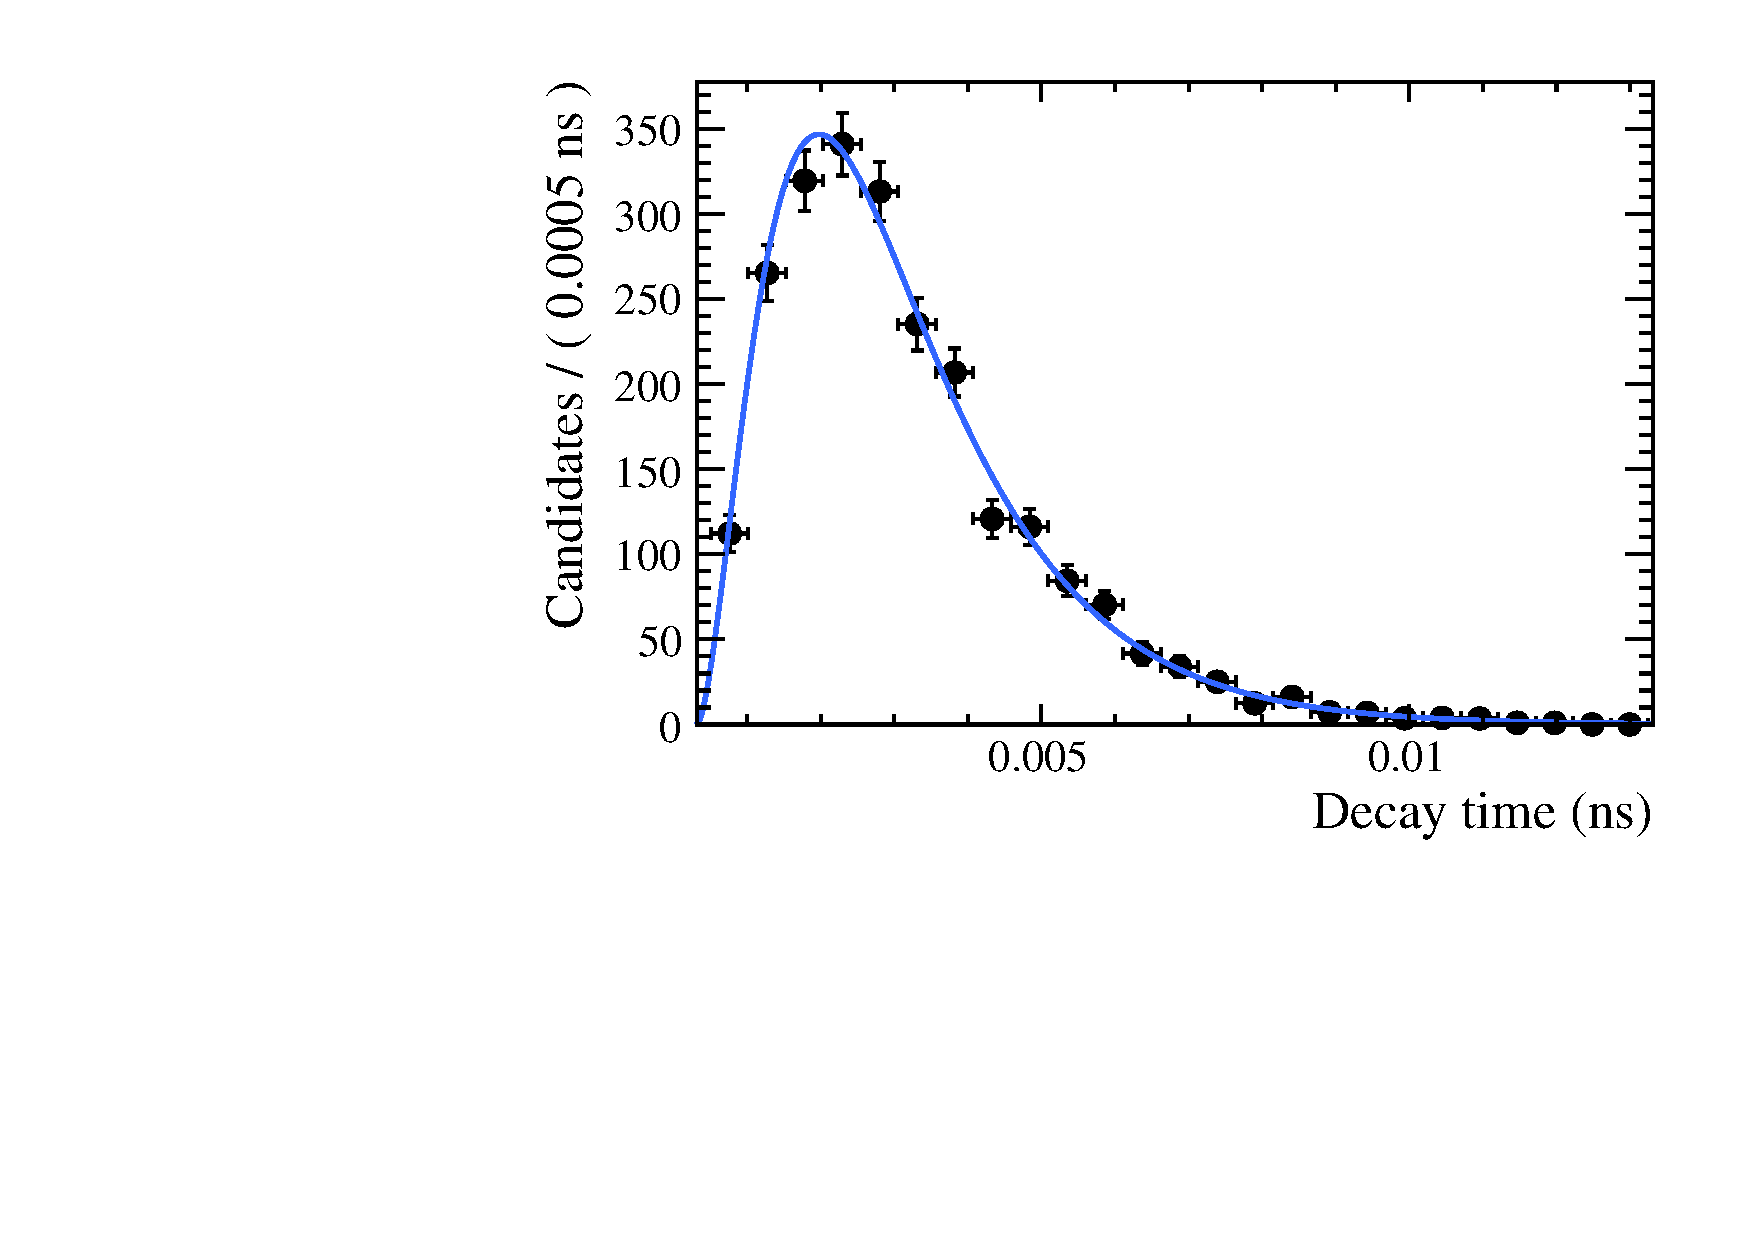
\includegraphics[width=0.6\textwidth]{./Figs/LifetimeSystematics/Bd2KPi_lifetime_fit.pdf}
\caption{Maximum likelihood fit to the signal weighted decay time distribution of \bskk decays for data taken in 2012 and 2015 data. }
\label{fig:bskklifetimefit}
\end{figure}

\section{Incorrectly assigned primary vertices and the detector resolution}
\label{sec:PVcheck}
Measuring the \bsmumu effective lifetime accurately relies on the $B^{0}_{s}$ candidate being assigned to the correct primary vertex in the event; an incorrect assignment would lead to the wrong value for the \bs decay time. % of an event.
In the references \cite{Aaij:2016ohx,Aaij:2015vza} that study the lifetimes of $B \to J/\psi X$ decays at LHCb, a component is included into the decay time fit to model the number of incorrectly assigned primary vertices (PVs) as well as the resolution of the detector. The decay time fit consists of a \pdf describing the decay time distribution convoluted by the sum of three Gaussian functions; two narrow Gaussian functions model the detector resolution  and a third wider Gaussian function corresponds to $<1\%$ of decays assigned incorrect PVs. The decay time fit to measure the \bsmumu \el does not explicitly model incorrectly assigned PVs or the detector resolution, although these effects will to some degree be included into the acceptance function. 

A similar model to the references~\cite{Aaij:2016ohx,Aaij:2015vza} is used to check the affect on the measured lifetime of decays with incorrectly assigned PVs and detector resolution effects that are not included in the acceptance function. A set of 1 million decays are generated using the decay time model 
\begin{equation}
\epsilon (t) [\mathcal{R}(t) \otimes e^{-t/\tau}],
\end{equation}
where $\epsilon (t)$ is the acceptance function with parameters given in Table \ref{tab:accptsig} and $\mathcal{R}(t)$ is the resolution function composed of 3 Gaussian functions. 
Decays are generated assuming the \bsmumu effective lifetime is equal to the lifetime of the heavy $B^{0}_{s}$ mass eigenstate of \tH = 1.610 \ps. A fit is then performed to the generated decay time distribution but  the resolution term is no longer included in the \pdf. The measured \tmumu value is compared to the value used to generate the decays. 


The resolution function is determined from weighted simulated \bsmumu decays that were used to compute the acceptance function in Section~\ref{sec:signalDTpdf}. The difference between the reconstructed decay time and the `true' decay time with which decays were generated is computed for each decay that passes the full selection. The resulting distribution is fitted with a resolution function composed of the sum of three Gaussian functions. Each Gaussian function has the same mean value, which is left free in the fit, but different widths that are also free in the final fit. The fit parameters are shown in Table \ref{tab:resolutionfit} and the results in Figure~\ref{}. % and the total fit in Figure \ref{fig:resolution_fit_plot}. 
The resulting distribution has a similar form to those used in references~\cite{Aaij:2016ohx,Aaij:2015vza}, where the detector resolution is modelled with two narrow Gaussian functions and the Gaussian function for incorrectly assigned PVs is broader and describes a small fraction of decays.


\begin{table}[ht]
\begin{center}
\begin{tabular}{lr}
\toprule \toprule
Parameter               & Fit value             \\ \midrule
$\mu$ (ps)              & 0.00063 $\pm$ 0.00005 \\ \midrule
$\sigma_{1} (ps)$       & 5.62$\pm$0.07         \\ 
$f_{1}$                 & 0.006               \\ \midrule
$\sigma_{2} (ps)$       & 0.0573$\pm$ 0.0003    \\ 
$f_{2}$                 & 0.313                \\ \midrule
$\sigma_{3} (ps)$       & 0.0294 $\pm$ 0.0001   \\ 
$f_{3}$                 & 0.681                \\ \bottomrule \bottomrule
\end{tabular}
\vspace{0.7cm}                                                                                    
\caption{Parameters from the fit to the difference between the reconstructed decay time and the true decay time for simulated decays that pass the \bsmumu \el selection. The mean used for all Gaussian is $\mu$ and $\sigma_{i}$ are the widths of each Gaussian that make up a fraction $f_{i}$ of the total sum.}
\label{tab:resolutionfit}
\end{center}
\vspace{-1.0cm}                                                                                   
\end{table}

\begin{figure}[htbp]
  \centering
    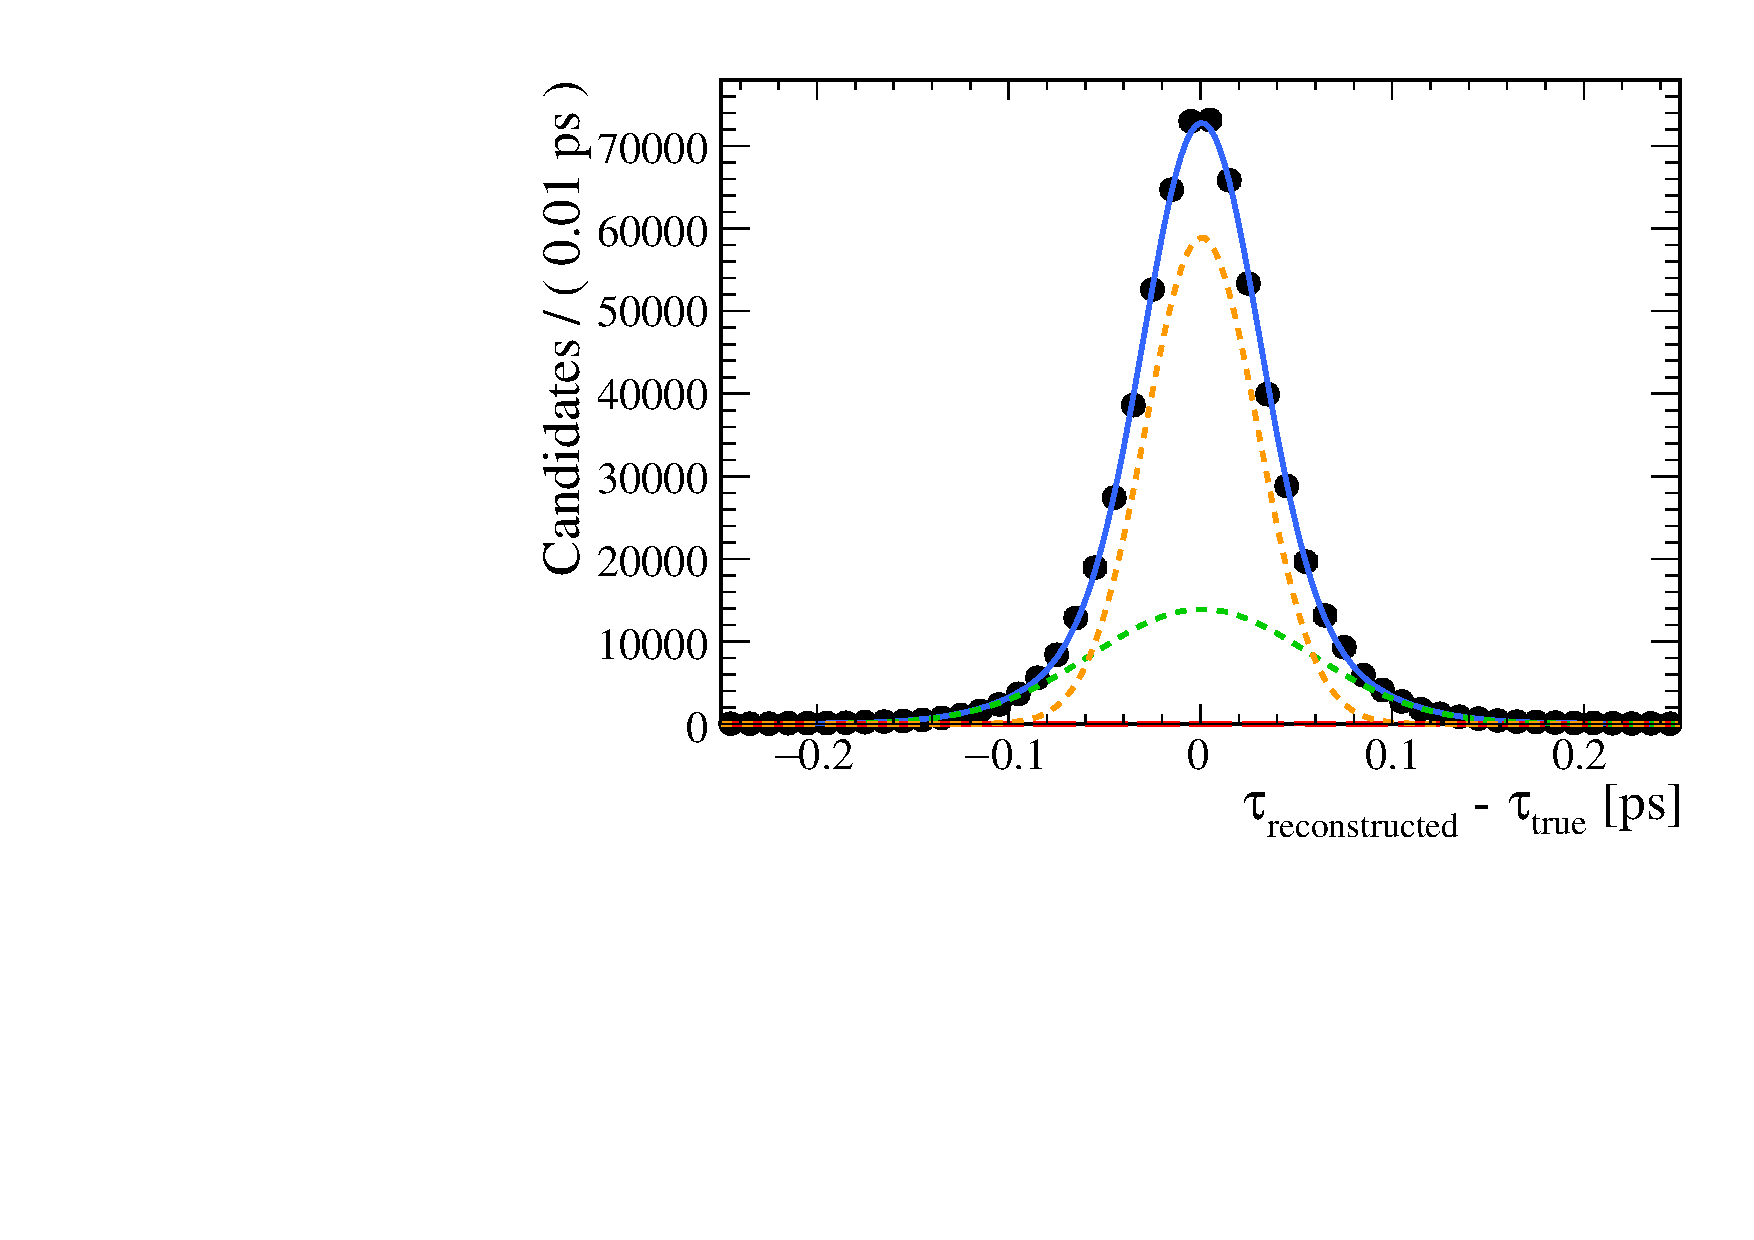
\includegraphics[width=0.6\textwidth]{./Figs/LifetimeSystematics/PV_decaytime_diff_fit.pdf}
  \caption{Fit result to the difference between the reconstructed decay time and the true decay time for simulated decays that pass the \bsmumu \el selection.}
  \label{fig:PVfit}
\end{figure}


The result from the fit to the generated decays without the resolution function included is \tmumu = 1.6098$\pm$ 0.0014 \ps, which is consistent with the lifetime of generate events. The difference between the lifetime used to generate events and the fitted value is 0.0002 ps, a factor of 10 smaller than the smallest systematic uncertainty. This cross check shows that the presence of incorrectly assigned PVs or detector resolution effects that are not included in the acceptance function have a negligible effect on the \bsmumu effective lifetime.



However, this check assumed that simulated decays provide a good estimate of the number of incorrectly assigned PVs. Figure~\ref{fig:Bd2KPi_nPVs_MC_data_comparison} shows the number of \bdkpi decays passing the selection for simulated \bdkpi decays and sWeighted decays data for each year. On average there are more PVs per event in simulated decays compared to data, therefore using simulation would give an overestimation of the number of incorrectly assigned PVs expected in data. 

\begin{figure}[htbp]
  \centering
    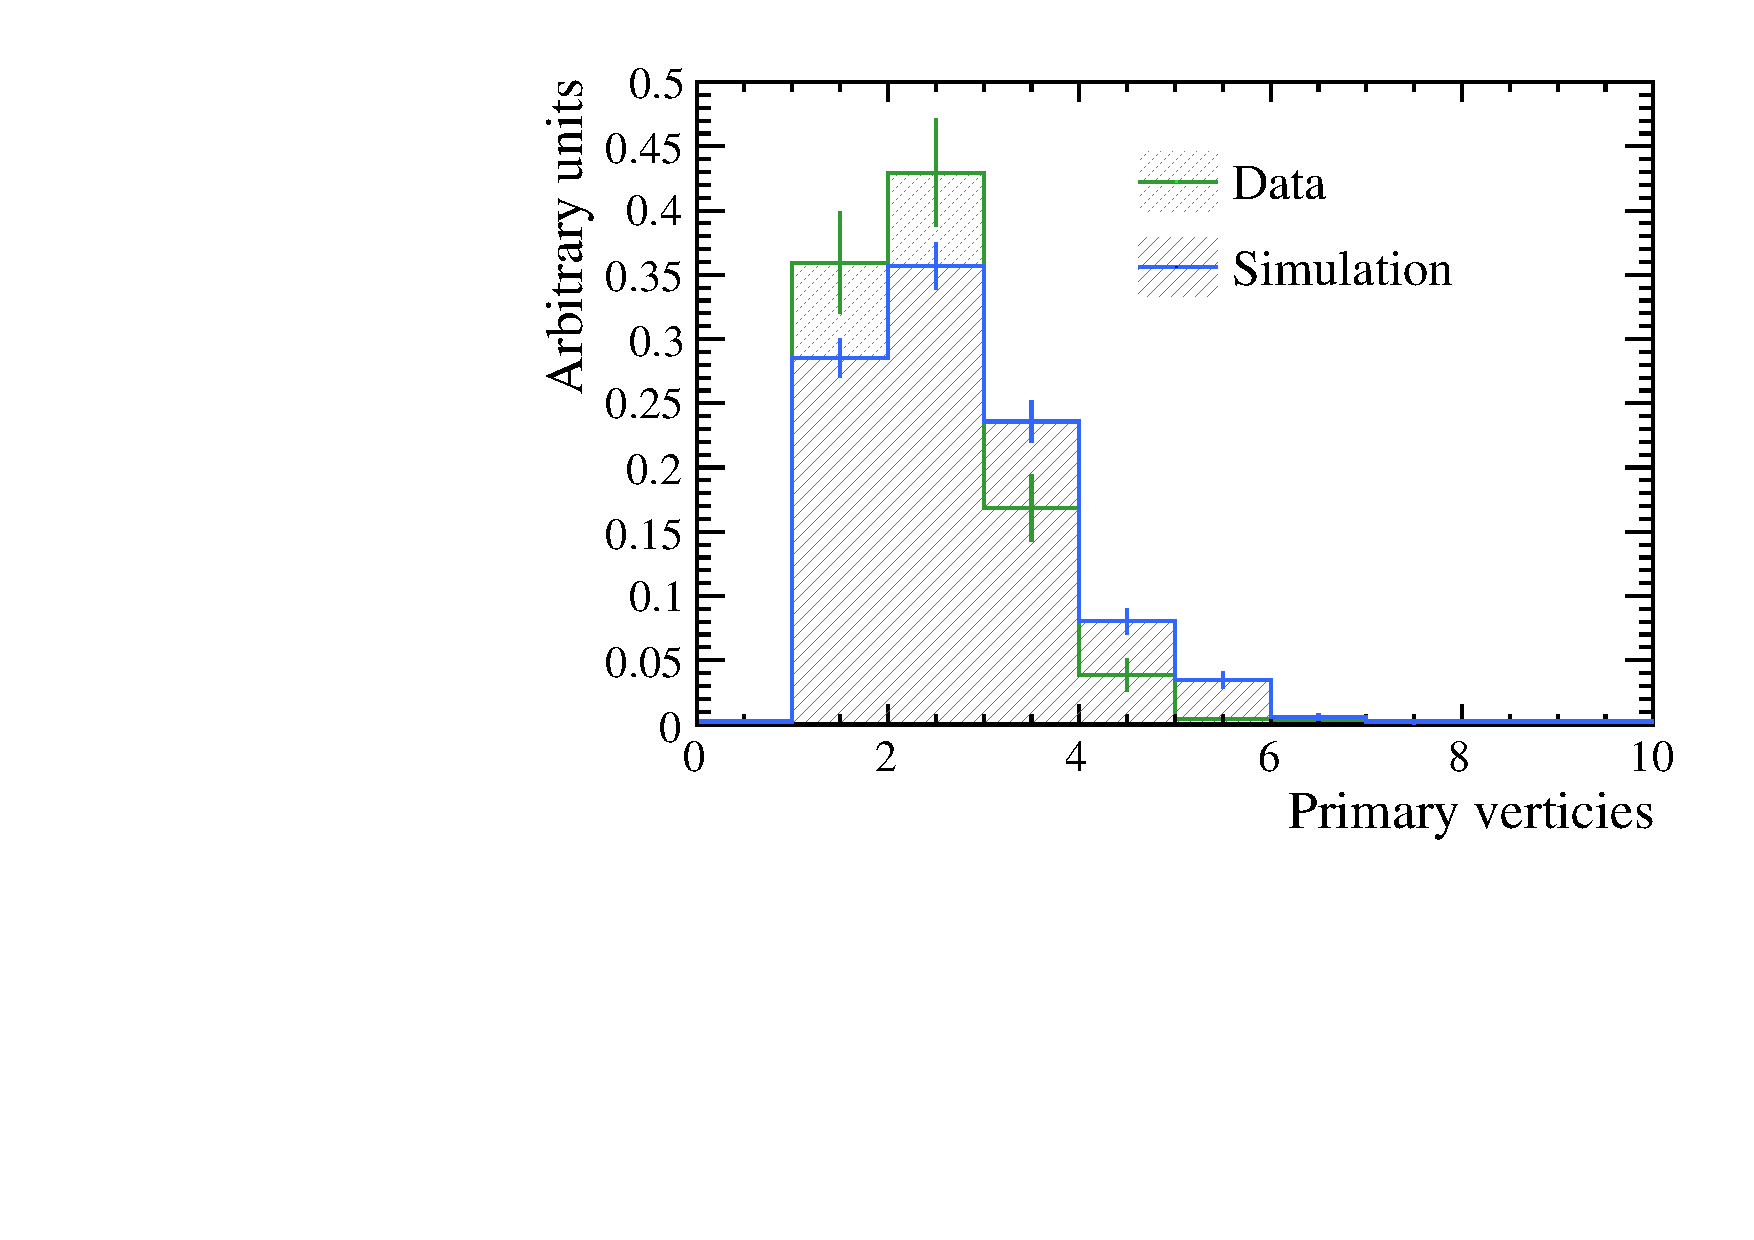
\includegraphics[width=0.49\textwidth]{./Figs/LifetimeSystematics/2011_nPVs.pdf}
    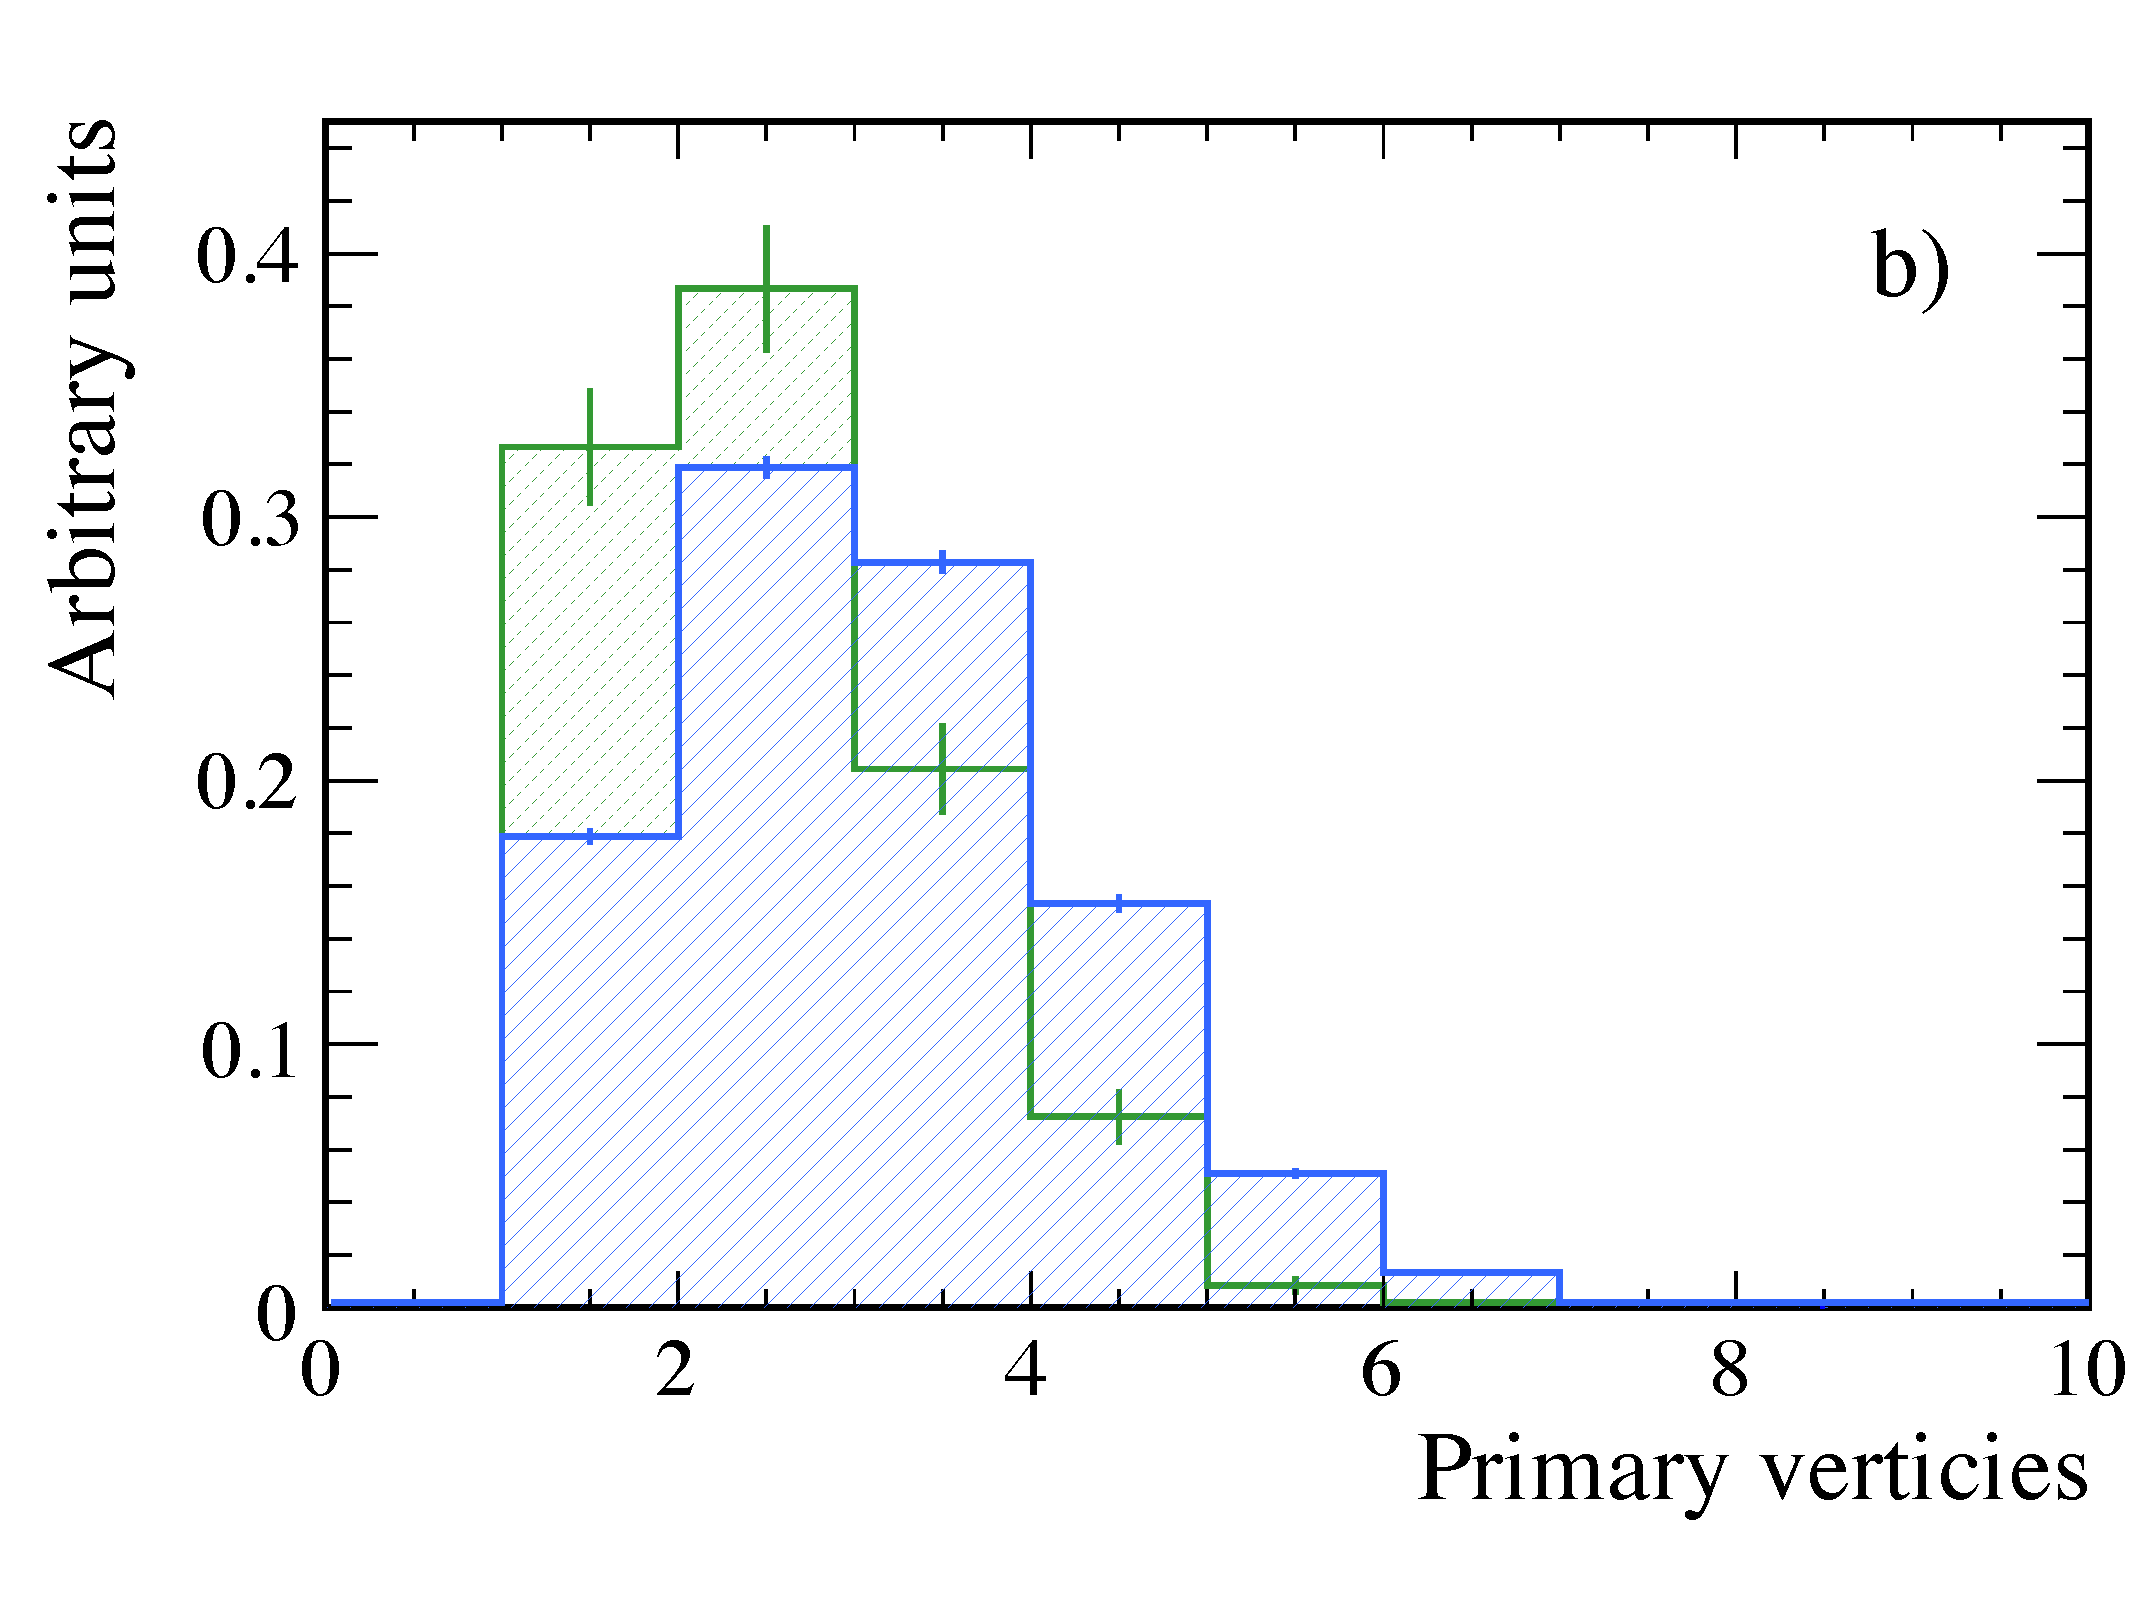
\includegraphics[width=0.49\textwidth]{./Figs/LifetimeSystematics/2012_nPVs.pdf}
    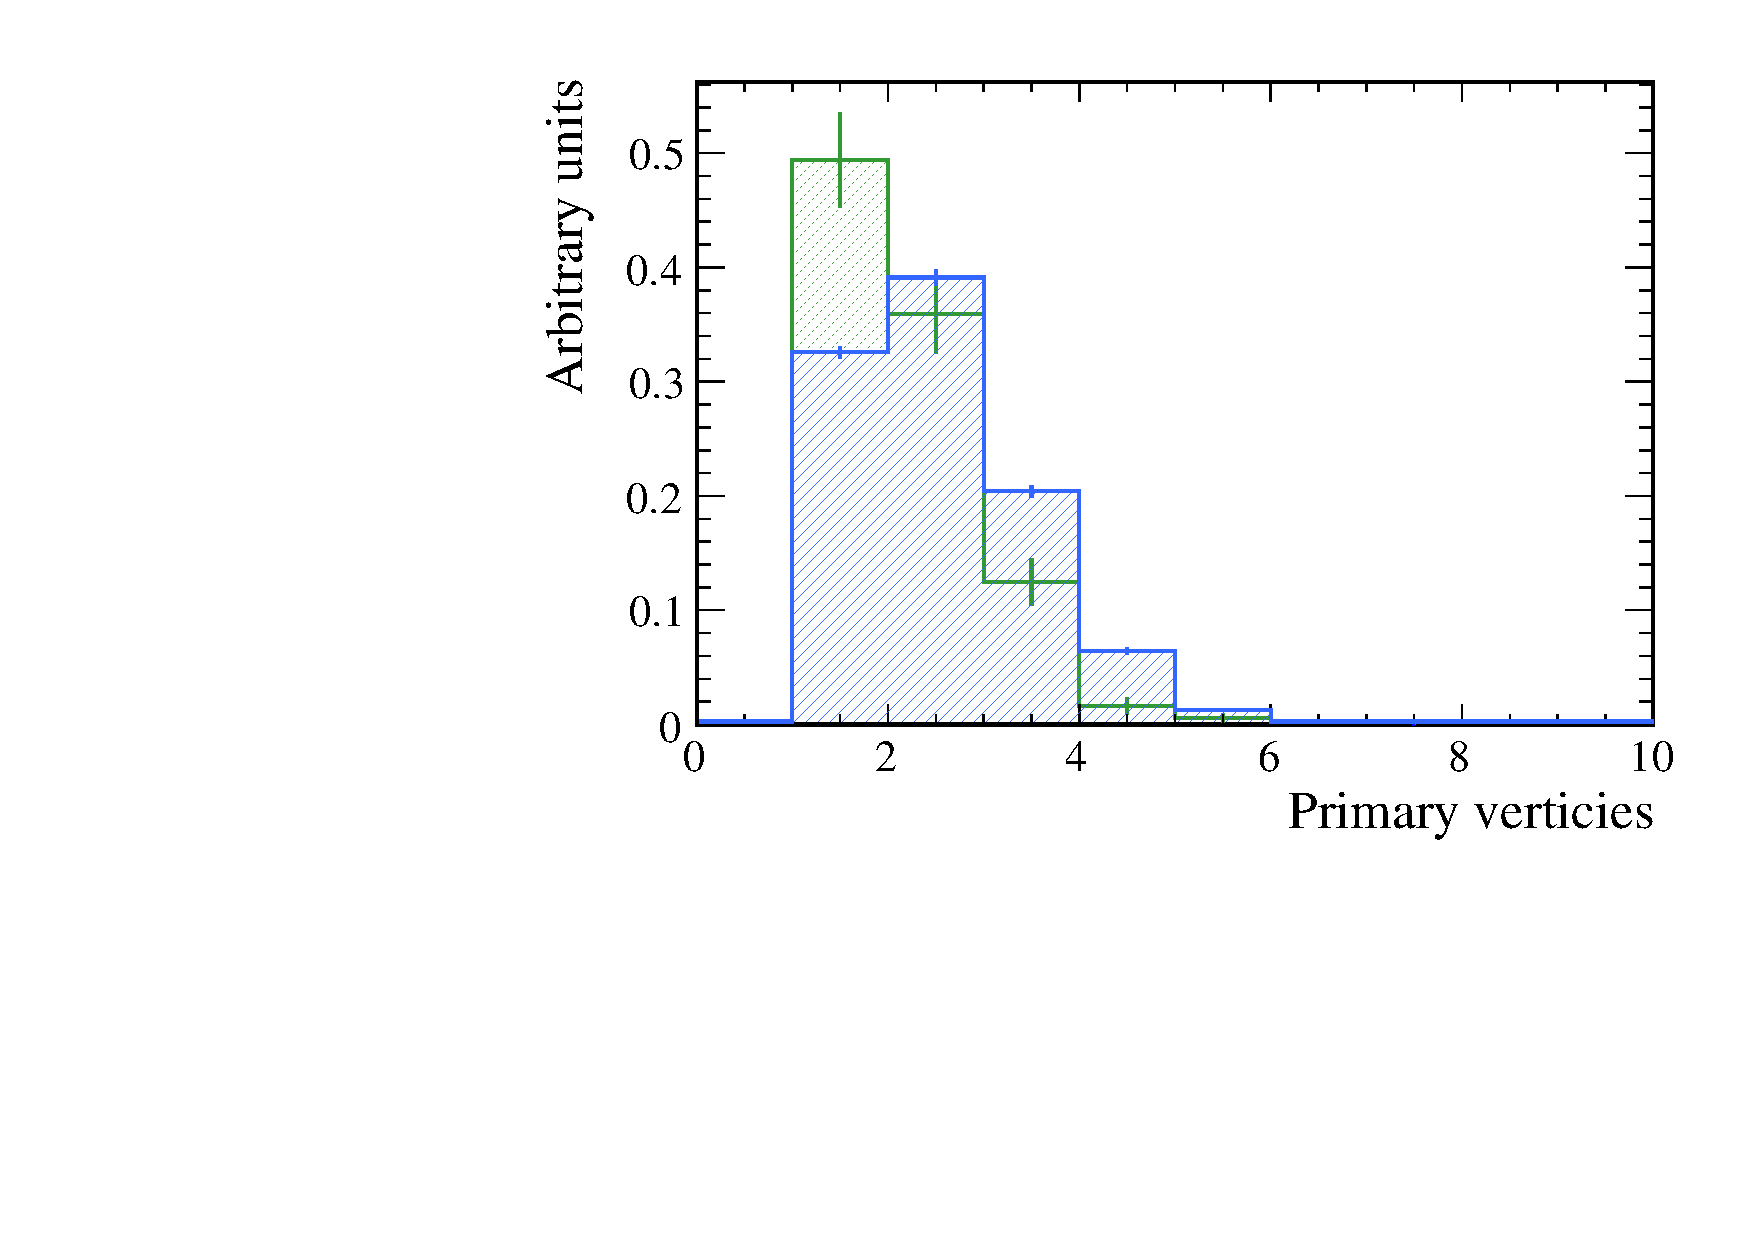
\includegraphics[width=0.49\textwidth]{./Figs/LifetimeSystematics/2015_nPVs.pdf}
    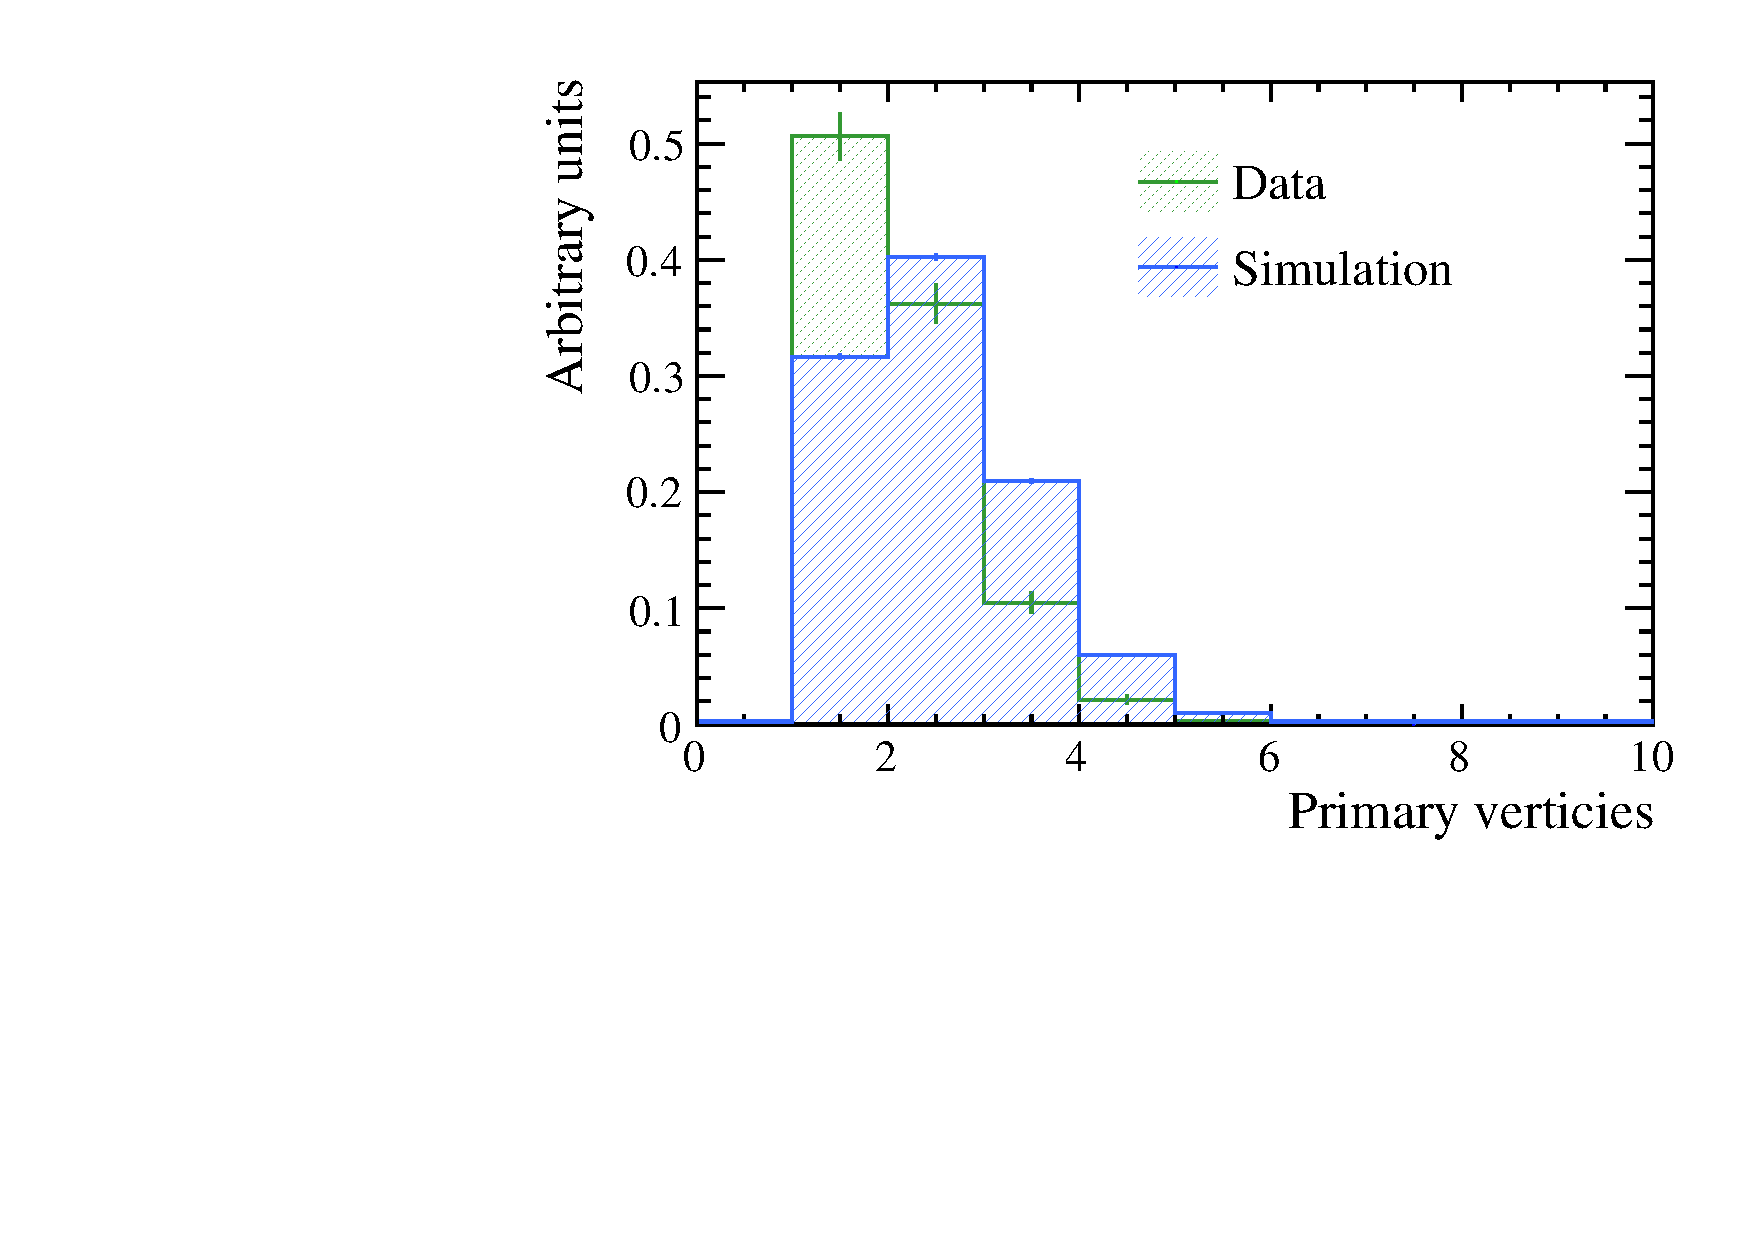
\includegraphics[width=0.49\textwidth]{./Figs/LifetimeSystematics/2016_nPVs.pdf}
  \caption{The distributions for the number of primary vertices in an event \bdkpi data and simulated decays for 2011 (top left), 2012 (top right), 2015 (bottom left) and 2016 (bottom right).}
  \label{fig:Bd2KPi_nPVs_MC_data_comparison}
\end{figure}


\section{Combinatorial background decay time model}
\label{sec:CBGdecytimemodel}

The decay time distribution of combinatorial background decays is largely unknown due to the nature of the background. The model used for this distribution in the pseudoexperiments is described in Section~\ref{sec:bkgDTpdf}. The decay time distribution of combinatorial background decays consists of mostly a short-lived component with a lifetime of 1.3 \ps and a long-lived component with a lifetime of 17 \ps.

The sWeighting method is sensitive to the background decay time components that are significantly longer lived than the signal lifetimes and can lead to a biased estimate of \tmumu. 
During the selection an upper decay time cut is applied to remove long-lived backgrounds. This cut is very effective at removing the bias entering the final results, although the remaining effect must be evaluated.

As discussed in Section~\ref{sec:bkgDTpdf} determining the decay time distribution of combinatorial background decays is challenging because there are too few decays left in either data or \bbbarmumux simulated decays after the selection requirements to determine the decay time \pdf. Therefore, the combinatorial background of \bhh decays in the mass range 5600 - 6000 \mevcc is used. The validity of using \bhh combinatorial background to model \bsmumu combinatorial background is studied by comparing the average lifetime of decays in bins of global BDT. The average lifetimes are shown in Table~\ref{tab:MeanDecayTimeBDTBins} for decays in data passing the selection requirements for \bsmumu and \bhh decays and in the mass ranges 5447 - 6000 \mevcc and 5600 - 6000 \mevcc, respectively. At low values of the global BDT the average lifetimes are similar and the lifetime of backgrounds of both decays increases with the output of the global BDT. Overall \bhh combinatorial background decays are longer lived than \bsmumu combinatorial background decays therefore the \bhh decay time model is a conservative estimate for \bsmumu combinatorial background as far as the affect of long-lived components in concerned. 


\begin{table}[htbp]
\begin{center}
\begin{tabular}{lrrrr}
\toprule \toprule
      & \multicolumn{2}{c}{\bsmumu} & \multicolumn{2}{c}{\bhh} \\ \midrule
BDT & mean decay      & Number of  & mean decay    & Number of \\
bin & time / \ps      & candidates & time / \ps    & candidates \\ \midrule 
1 & $1.178 \pm 0.005$ & 50,695 & $1.124 \pm 0.001$ & 964,502 \\
2 & $1.936 \pm 0.098$ &    244 & $2.394 \pm 0.022$ & 8,838 \\
3 & $2.570 \pm 0.327$ &     46 & $2.781 \pm 0.051$ & 2,373 \\
4 & $2.210 \pm 0.361$ &     17 & $3.023 \pm 0.076$ & 1,125 \\
5 & $2.582 \pm 1.103$ &      4 & $3.417 \pm 0.112$ &   655\\
6 & $2.540 \pm 0.390$ &      3 & $3.978 \pm 0.187$ &   313\\
7 & $2.868 \pm 1.048$ &      2 & $4.626 \pm 0.363$ &   109\\
8 & -                 &      0 & $5.706 \pm 0.683$ &    35\\ \bottomrule \bottomrule
\end{tabular}
\vspace{0.7cm}
\caption{The mean decay time of \bsmumu and \bhh candidates in 2011, 2012, 2015 and 2016 data in bins of the global BDT output. The mass ranges 5447 - 6000 \mevcc and 5600 - 6000 \mevcc are used for \bsmumu and \bhh decays, respectively.}
\label{tab:MeanDecayTimeBDTBins}
\end{center}
\vspace{-1.0cm}
\end{table}

The model used for the combinatorial background decay time currently introduces no significant bias into the pull distribution of \Gmumu for pseudoexperiments as shown in Table~\ref{tab:toyResults}. However, the size of a systematic bias from uncertainties in the decay time distribution is estimated by two sets of pseudoexperiments. The first uses the background decay time distribution in Table~\ref{tab:bkgparams} and the second set uses a modified verion this distribution: $\tau_1$ and $\tau_2$ are both increased by 1$\sigma$; and the fraction of decays with lifetime $\tau_1$ is increased by 1$\sigma$. For both sets of pseudoexperiments only combinatorial background and \bsmumu decays are generated and 10,000 studies are performed for each configuration. 

The resulting pull distributions for \Gmumu are shown in Figure~\ref{fig:CBGextreme}, the difference in the mean value of the distributions for the two studies is negligible and the width changes by 0.008 \ps$^{-1}$ between the two studies. The change in the width is the largest and therefore the systematic uncertainty is estimated from this. Assuming the expected uncertainty for \tmumu a systematic uncertainty of 0.002~\ps is assigned due to the combinatorial background decay time model.

\begin{figure}[htbp]
  \centering
    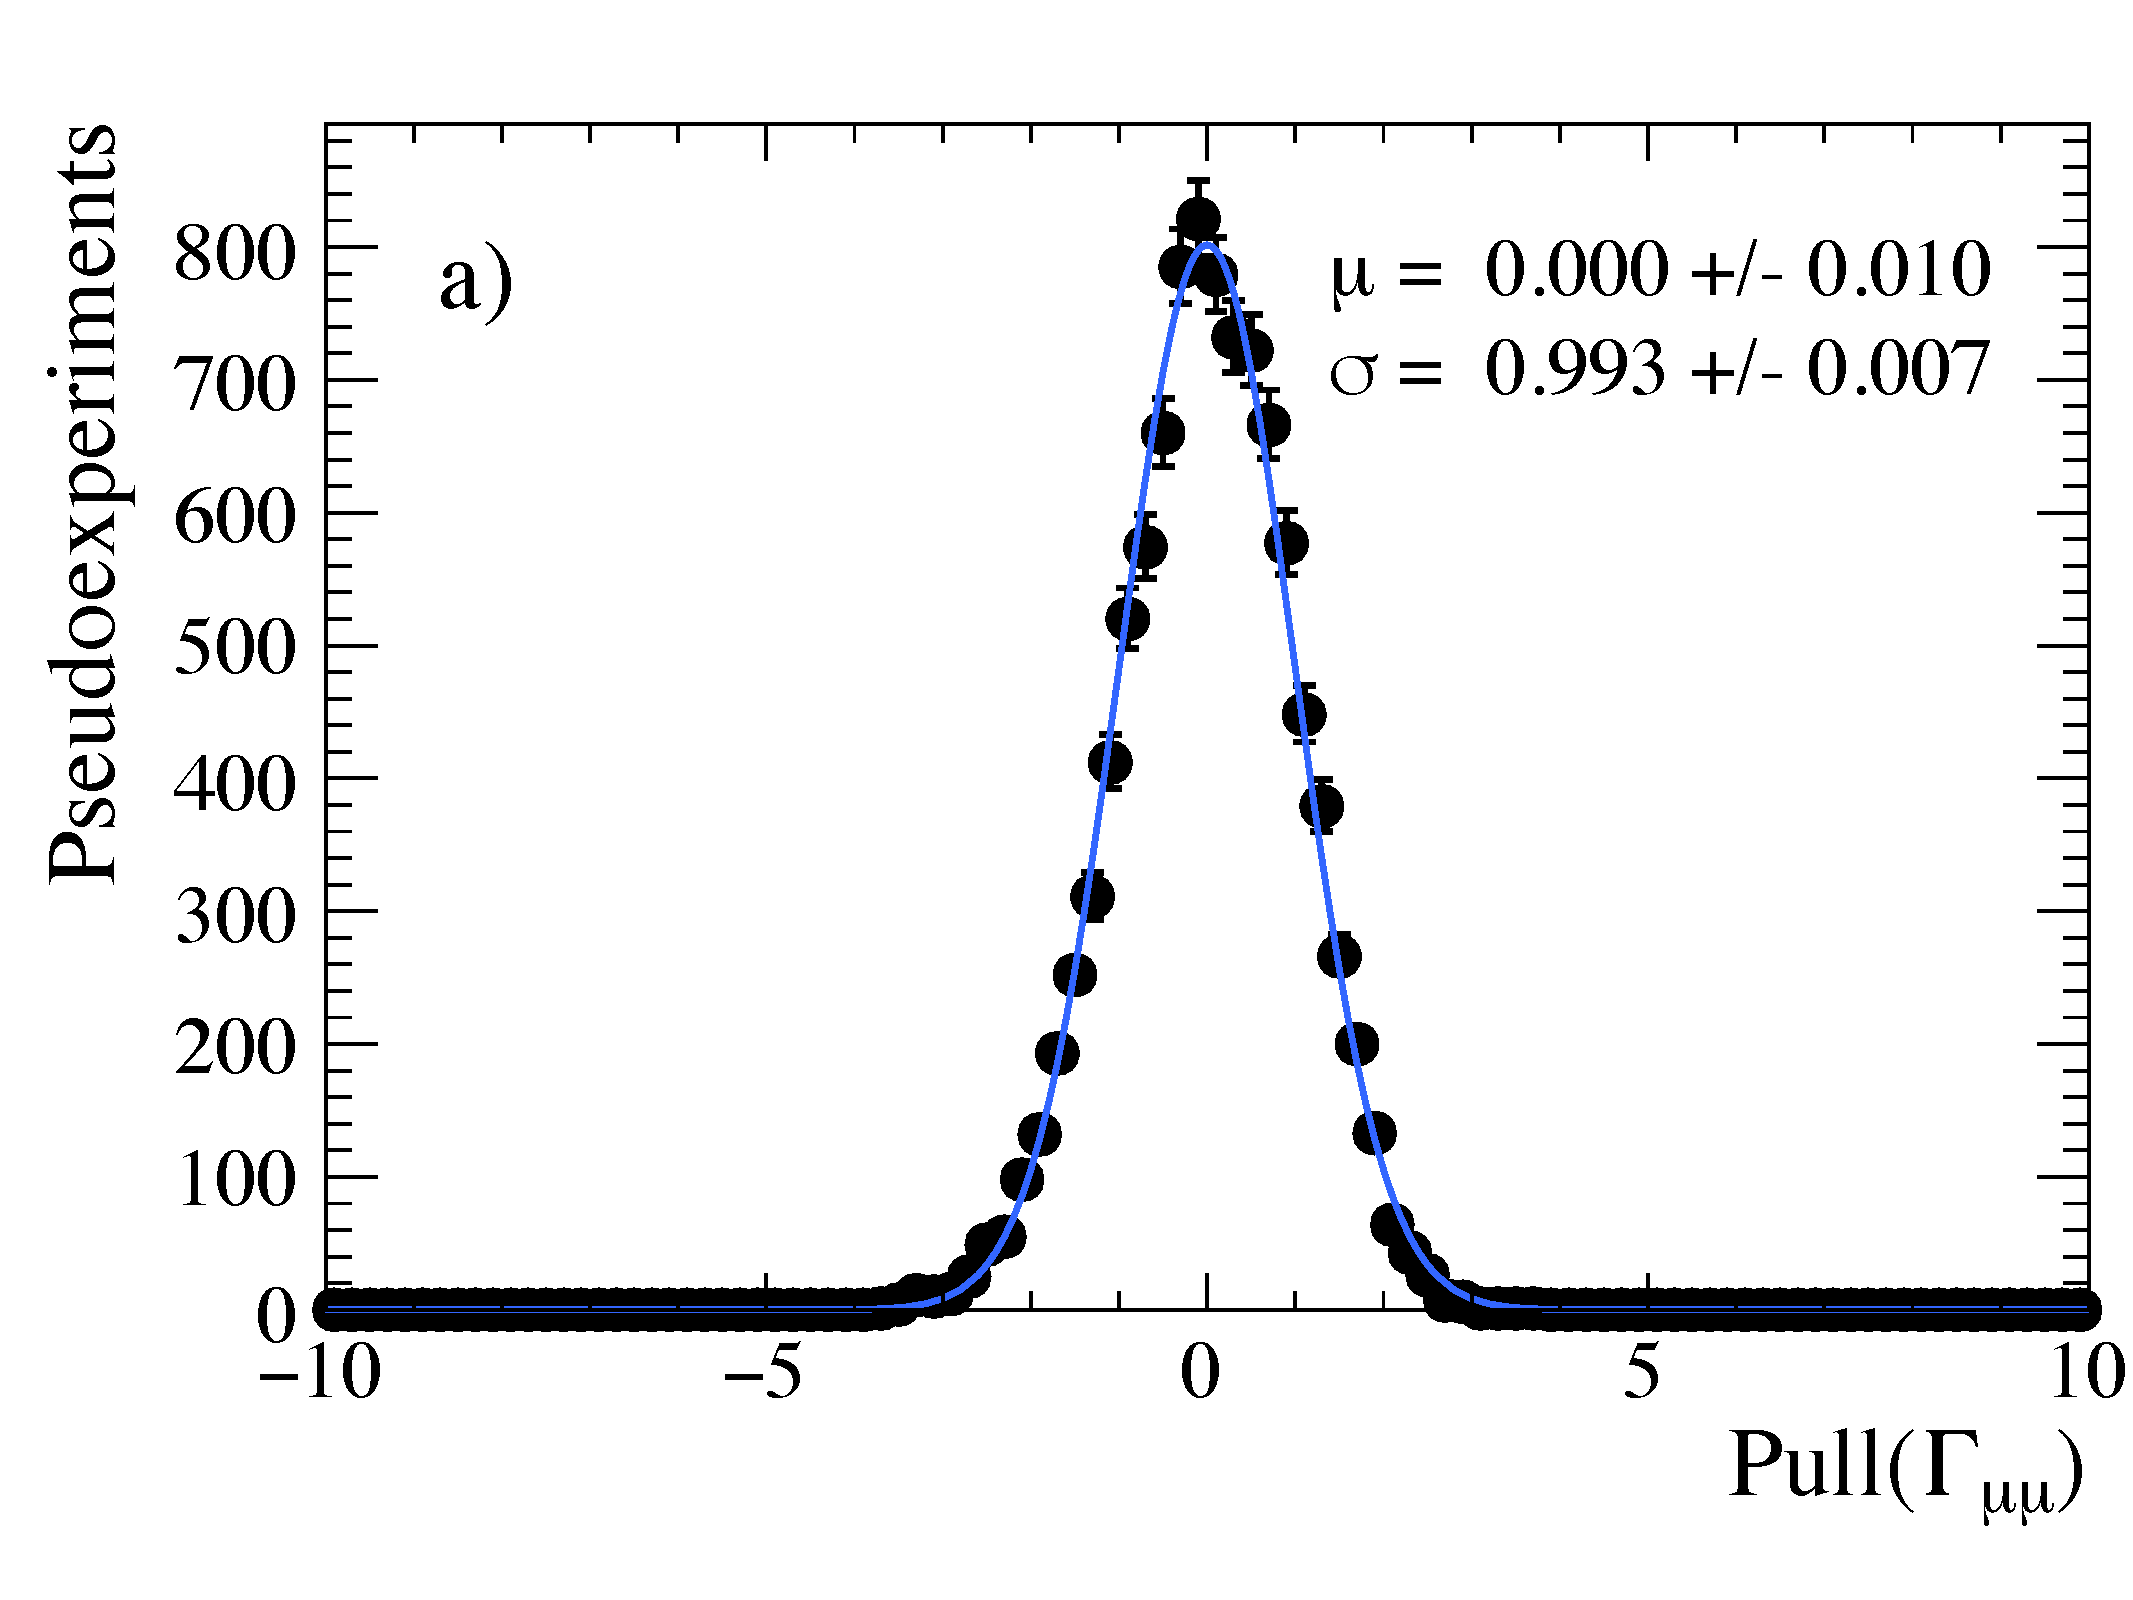
\includegraphics[width=0.49\textwidth]{./Figs/LifetimeSystematics/Gamma_pull_mass_pdf_Run1.pdf}
    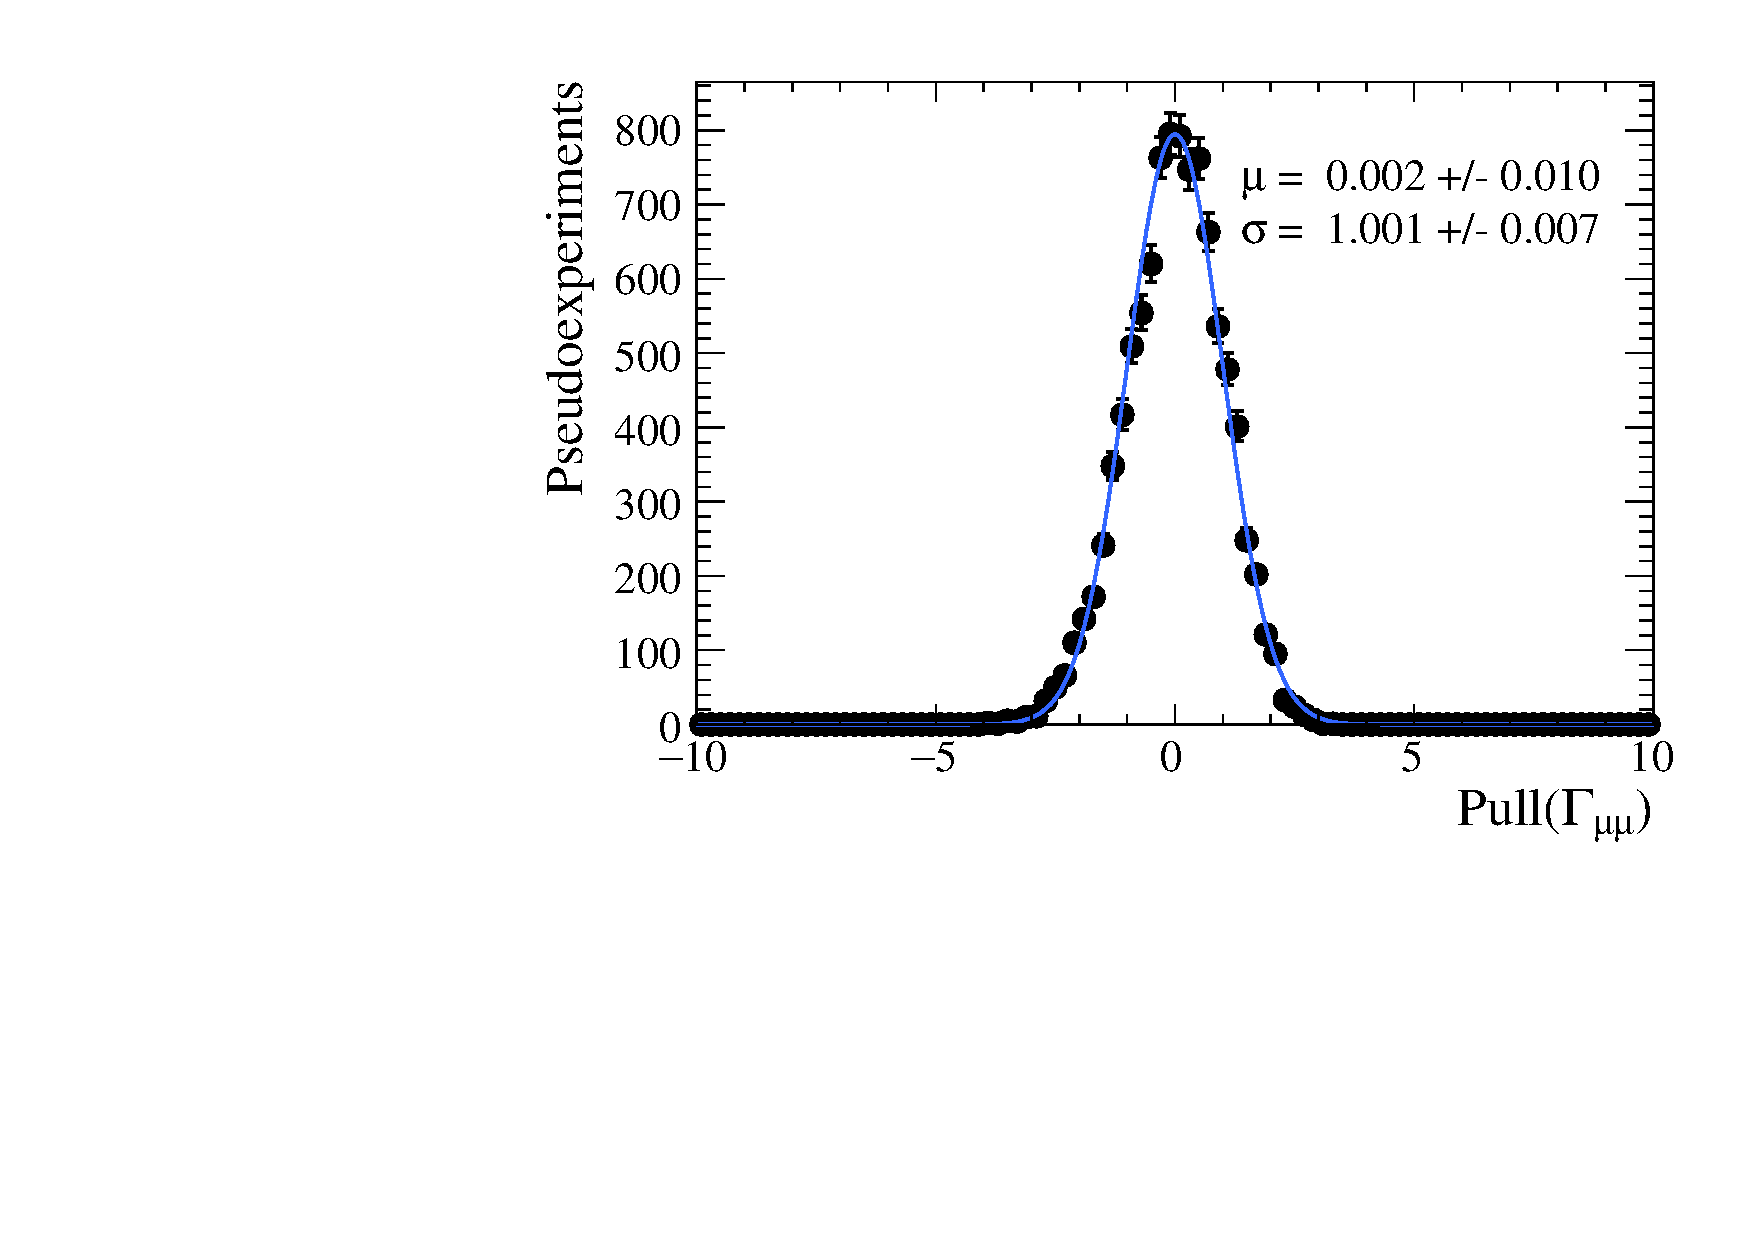
\includegraphics[width=0.49\textwidth]{./Figs/LifetimeSystematics/Bs2MuMu_gamma_pull_CKM_extremeCBG_DT.pdf}
  \caption{Pull distributions for \Gmumu from 10,000 pseudoexperiments using the nominal combinatorial background decay time model (left) and the nominal model with the lifetimes and fraction of longer lived decays increased by one standard deviation (right).}
  \label{fig:CBGextreme}
\end{figure}


\section[Mix of \bs mass eigenstates]{Mix of \boldmath{\bs} mass eigenstates}
\label{sec:mixofeigenstates}

In the Standard Model the \bsmumu \el is equal to the lifetime of the heavy \bs mass eigenstate. However, the real \bsmumu \el could be different due to the mixture of the light and heavy mass eigenstates. %The expected PDG values for the different lifetimes are \tH = and \tL = .

As shown in Section~\ref{sec:DTpdfs} the selection efficiency used to identify \bsmumu candidates is not uniform across the decay time range. The selection rejects a greater proportion of candidates with short lifetimes compared to candidates with longer lifetimes. Therefore, the presence of the light \bs mass eigenstate decaying as \bsmumu could be masked by the bias in the decay time distribution, since the efficiency to select the light \bs mass eigenstate is lower than the efficiency to select the heavy \bs mass eigenstate.

The size of this effect has been estimated using two simple pseudoexperiments. The first assumes that the selection has no bias on the decay time distribution and 1 million candidates are generated with equal contributions from the heavy and light \bs mass eigenstates. % Therefore assuming even missing of the light and heavy mass eigenstates contribution to \bsmumu decays. 
 A second set of 1 million candidates are generated with the same mix of eigenstates but with a more realistic model including the \bsmumu acceptance function. A fit is performed to the first set of candidates with a single exponential function and the second set with the acceptance function and exponential function in order to find \tmumu for each distribution. The acceptance parameters are fixed in the second fit.

The values of \tmumu are compared for the two studies and a systematic uncertainty is assigned for the change in \tmumu caused by the inclusion of the acceptance function. The fit results are shown in Figure~\ref{fig:mixofstates} and the difference between the measured lifetimes for the two studies is 0.018~\ps.

\begin{figure}[htbp]
  \centering
    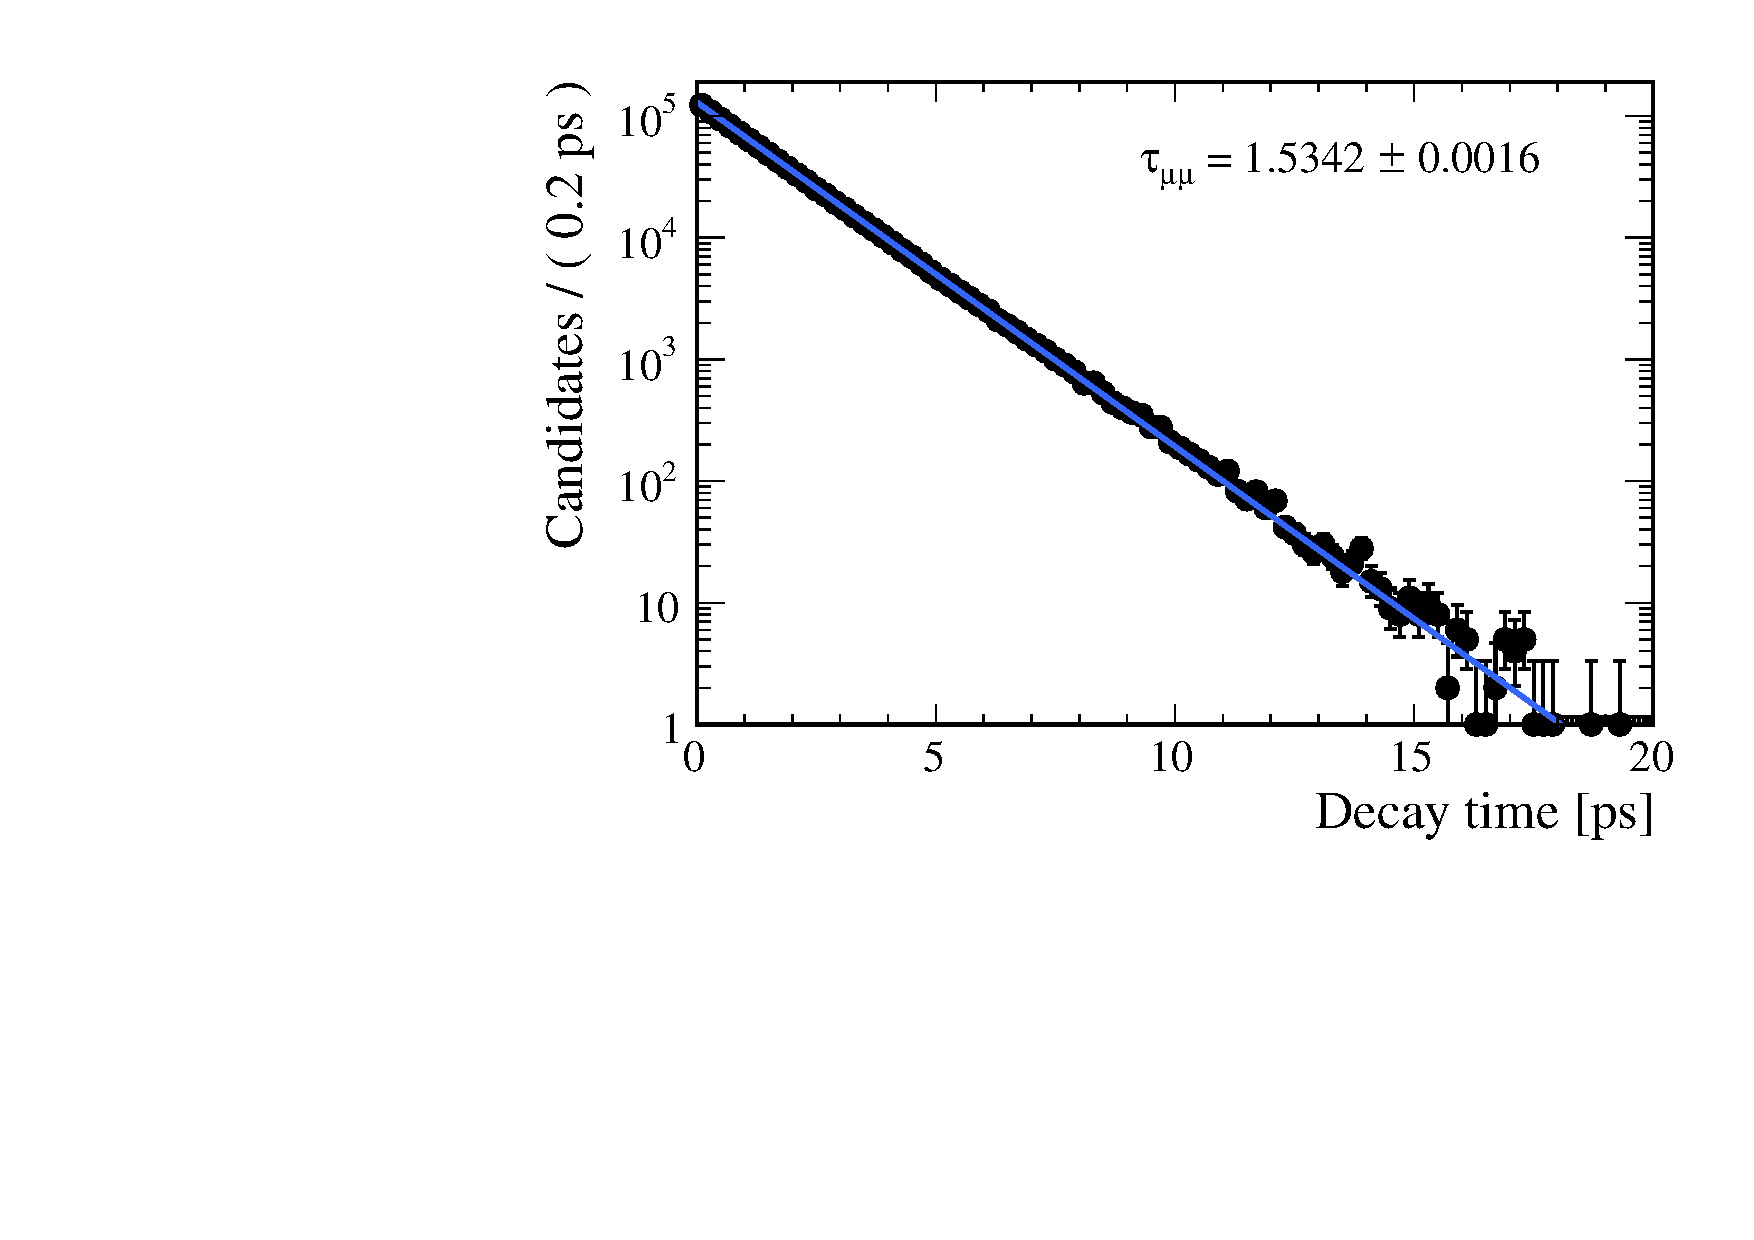
\includegraphics[width=0.49\textwidth]{./Figs/LifetimeSystematics/No_acc_fit.pdf}
    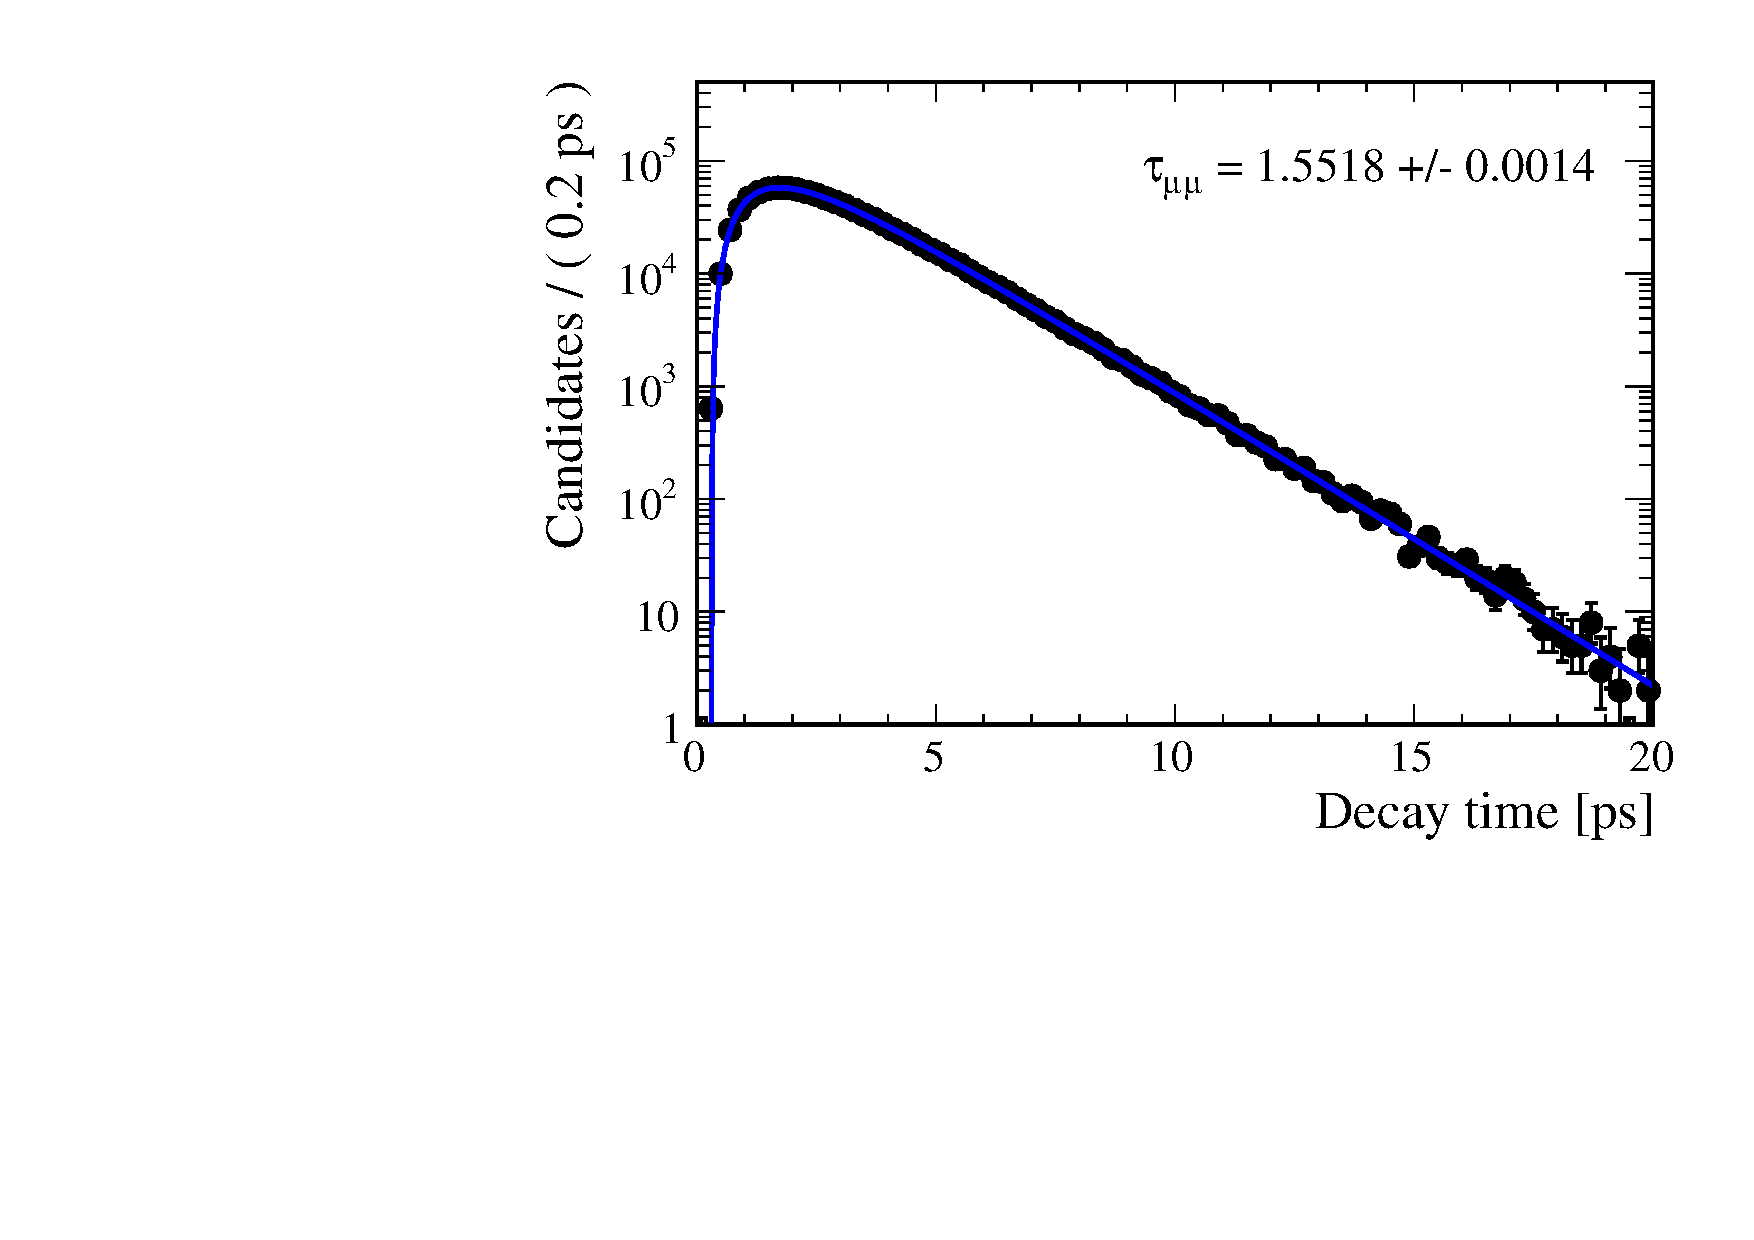
\includegraphics[width=0.49\textwidth]{./Figs/LifetimeSystematics/Acc_fit.pdf}
  \caption{Maximum likelihood fits to the decay time distribution to measure \tmumu for \bsmumu decays that are composed of an equal mix from the heavy and light mass eigenstates. Decay time distributions are generated assuming a flat acceptance function (left) and the acceptance function used to describe \bsmumu decays in data (right).}
  \label{fig:mixofstates}
\end{figure}


\section[Production asymmetry of \bs and $\overline{B}_{s}^{0}$}]{Production asymmetry of \boldmath{\bs} and \boldmath{$\overline{B}_{s}^{0}$}}
\label{sec:productionasymetry}

%The effective lifetime is defined as (some words) and is given by the following equation.
%Our measurement assumes that the decay time rate is given by (this) 
%however this assume that Bs and anti-Bs are produced in equal proportions, this is not the case for a pp collider
%The decay rate is actually given by this where the Ap is the production asymmetry which is given by
%LHCb has measured this as X at 7 TeV, we assume that is it indenepdant of energy - is it/is that obvious?
%Therefore as a systematic uncertainty we evaluate the base intofirced by the mix of eigenstates
%as written in the theory chapter the decay rates of the Bs and the anti-Bs are given by the following
%Therefore leading to a total decay rate in the presence of production asymeter of the following
%w%here we have assumed the standard relationships between Gamma_s, L and H
%look there is not an extra oscillating term here that wasn’t there in the theory chapter.
%By integrating by parts the components used in the effective lifetime are now the following
%The bias introduced by the production asymeter is evaluated using these parameters from the PDG and also assuming Ap = ? and A_DG = ?.


The \bsmumu effective lifetime is the mean lifetime of an unbiased sample of \bsmumu decays, as discussed in Chapter~\ref{sec:theory}, and is given by
\begin{equation}
 \tau_{\mu\mu} \equiv \frac{\int^\infty_0 t \left<\Gamma \left( B^{0}_s(t) \rightarrow \mu^{+} \mu^{-} \right) \right> dt }{\int^\infty_0 \left<\Gamma \left( B^{0}_s(t) \rightarrow \mu^{+} \mu{-} \right) \right> dt },
\label{eq:el}
\end{equation}
where the untagged decay rate is
\begin{equation}
\left< \Gamma \left( B^0_s(t) \rightarrow \mu^{+} \mu^{-} \right)\right>  = \Gamma \left ( B^0_s(t) \rightarrow \mu^{+}\mu^{-} \right) + \Gamma \left ( \bar{B^0_s}(t) \rightarrow \mu^{+} \mu^{-} \right),
\end{equation}
and assumes that \bs and $\overline{B}^{0}_{s}$ mesons are produced at equal rates. This assumption is made for the measured value of \tmumu. However, since the LHC is a $pp$ collider, \bs and $\overline{B}^{0}_{s}$ mesons are not produced at equal rates. The affect of such a production asymmetry of \bs and on the measured results must therefore be evaluated. 

The production asymmetry is given by 
\begin{equation}
 A_{p} \equiv \frac{\sigma\left(B^{0}_{s}\right) - \sigma\left(\overline{B}^{0}_{s}\right)}{\sigma\left(B^{0}_{s}\right) + \sigma\left(\overline{B}^{0}_{s}\right)},
\label{eq:Ap}
\end{equation}
where $\sigma\left(B^{0}_{s}\right)$ and $\sigma\left(\overline{B}^{0}_{s}\right)$ are the production cross-sections for \bs and $\overline{B}^{0}_{s}$ mesons, respectively. The production asymmetry was measured by LHCb in 2011 at a centre of mass energy of 7~TeV as $ A_{p} = (1.09 \pm 2.61 \pm 0.66) \%$ \cite{Aaij:2014bba}. The presence of the production asymmetry modifies the \bsmumu decay rate to
\begin{align}
\Gamma\left( B^0_s(t) \rightarrow \mu^{+}\mu^{-}\right) = \left(\frac{1+A_p}{2}\right)&\Gamma(B^0_s(t)\rightarrow \mu^{+} \mu^{-}) \nonumber \\
&  + \left(\frac{1-A_p}{2}\right)\Gamma(\overline{B}^0_s(t)\rightarrow \mu^{+} \mu^{-}).
\label{eq:modifieddecayrate}
\end{align}

The affect of the production asymmetry on the measured lifetime is determined from Equations~\ref{eq:el} and~\ref{eq:modifieddecayrate} using the decay rates of \bsmumu and $\overline{B}^{0}_{s} \to \mu^{+} \mu^{-}}$ given in Equations~\ref{eq:decayratesApart} and~\ref{eq:decayratesA}.
%\begin{eqnarray}
% \Gamma(B^0_s(t)\rightarrow \mu^{+} \mu^{-}) &=& \frac{1}{2}N_{\mu^{+} \mu^{-}} |A_{\mu^{+} \mu^{-}}|^2 (1+|\epsilon|^2)e^{-\Gamma_{s} t} \bigg\{ \cosh \frac{\Delta\Gamma_{s} t}{2} + \nonumber \\ 
%& & C_{\lambda} \cos(\Delta m_{s} t) + A_{\Delta\Gamma}^{\mu^{+}\mu^{-}} \sinh \frac{\Delta\Gamma_{s} t}{2} + \nonumber \\
%& & S_{\lambda} \sin(\Delta m_{s} t) \bigg\}, \\ 
% \Gamma(\overline{B}^{0}_{s}(t)\rightarrow \mu^{+} \mu^{-} ) &=& \frac{1}{2}N_{\mu^{+} \mu^{-}} |A_{\mu^{+} \mu^{-}}|^2 (1+a) (1+|\epsilon|^2)e^{-\Gamma_{s} t} \bigg\{ \cosh \frac{\Delta\Gamma_{s} t}{2} \nonumber \\
%& & - C_{\lambda} \cos(\Delta m_{s} t) + A_{\Delta\Gamma}^{\mu^{+} \mu^{-}} \sinh \frac{\Delta\Gamma_{s} t}{2} - \nonumber \\
%& & S_{\lambda} \sin(\Delta m_{s} t) \bigg\}  
%\end{eqnarray}



The total decay rate with the production asymetry is
\begin{eqnarray}
 \Gamma\left( B^0_s(t) \rightarrow \mu^+\mu^-\right) %&=& \left(\frac{1+A_p}{2}\right)\Gamma(B_s^0(t)\rightarrow \mu^+ \mu^-) + \left(\frac{1-A_p}{2}\right)\Gamma(B^0_s(t)\rightarrow \mu^+ \mu^-) \nonumber \\ 
             &= \frac{1}{2}\mathcal{N} |A_{\mu \mu}|^2 (1+|\lambda_{\mu\mu}|^2)e^{-\Gamma_{s} t} \bigg\{ \cosh \left( \frac{\Delta\Gamma_{s} t}{2}\right)  +A_{\Delta\Gamma} \sinh \left(\frac{\Delta\Gamma_s t}{2}\right) \nonumber \\
&\quad{}+ A_p [ C_{\lambda} \cos(\Delta m_{s} t)+ S_{\lambda} \sin(\Delta m_s t)] \bigg\} + \mathcal{O}(a),

\end{align}
where $C_{\lambda} = (1 - |\lambda_{\mu\mu}|^2)/(1 + |\lambda_{\mu\mu}|^2)$ and $S_{\lambda} = 2\mathrm{Im}/(1 + |\lambda_{\mu\mu}|^2)$ are $\mathcal{CP}$ asymmetries and are related to \ADG by $|A_{\Delta\Gamma}|^2 + |C_{\lambda}|^2 + |S_{\lambda}|^2 = 1$~\cite{Anikeev:2001rk}.

The production asymmetry introduces an additional oscillatory term which disappears when $A_p=0$. % ~\ref{}.
Using the relationships $\Delta\Gamma_{s} = \Gamma_{L} - \Gamma_{H}$ and $\Gamma_{s} = (\Gamma_{L} + \Gamma_{H})/2$ and ignoring terms $\mathcal{O}(a)$, the decay rate becomes
\begin{align}
\label{eqn:BsmmDoubleExpoWithAp}
 \Gamma\left( B^{0}_{s}(t) \rightarrow \mu^{+} \mu^{-}\right) &\simeq \mathcal{N}’ \bigg\{ (1-A_{\Delta\Gamma})e^{-\Gamma_{L} t} + (1+A_{\Delta\Gamma})e^{-\Gamma_{H} t} \nonumber \\
& \quad {} + 2A_p e^{-\Gamma_{s} t} \left[ C_{\lambda} \cos(\Delta m_{s} t) + S_{\lambda} \sin(\Delta m_{s} t) \right] \bigg\},
\end{align}
where $\mathcal{N}' \equiv \frac{1}{4}\mathcal{N} |A_{\mu \mu}|^2 (1+|\lambda_{\mu\mu}|^2)$. 
This decay rate can be used to calculate the \bsmumu effective lifetime in the presence of a production asymmetry. Using integration by parts the contributing terms to the effective lifetime become
\begin{align}
 \int_0^\infty t \left<\Gamma\left( B^0_s(t) \rightarrow \mu^{+} \mu^{-}\right)\right> dt = &\mathcal{N}' \bigg\{ \frac{1-A_{\Delta\Gamma}}{\Gamma_{L}^2} + \frac{1+A_{\Delta\Gamma}}{\Gamma_{H}^{2}} \\
&\quad {}+ \frac{2A_p}{(\Delta m_{s}^2 + \Gamma_{s}^2)^2} \left [C_{\lambda}(\Gamma_{S}^2 - \Delta m_{s}^2) + 2S_{\lambda} \Gamma_{S} \Delta m_{s} \right ] \bigg\} \nonumber
\end{align}
%\begin{eqnarray}
% \int_0^\infty t \left<\Gamma\left( B^0_s(t) \rightarrow \mu^{+} \mu^{-}\right)\right> dt = &N'& \bigg\{ \frac{1-A_{\Delta\Gamma}^{\mu^{+} \mu^{-}}}{\Gamma_{L}^2} + \frac{1+A_{\Delta\Gamma}^{\mu^{+} \mu^{-}}}{\Gamma_{H}^{2}} \nonumber \\
%&+& 2A_p \left [C_{\lambda}\frac{\Gamma_{S}^2 - \Delta m_{s}^2}{(\Delta m_{s}^2 + \Gamma_{s}^2)^2} \nonumber \\
%&+& S_{\lambda}\frac{2 \Gamma_{S} \Delta m_{s}}{(\Delta m_{s}^2 + \Gamma_{S}^2)^2} \right] \bigg\}
%\end{eqnarray}

and
\begin{align}
 \int_0^\infty \left<\Gamma\left( B_s(t) \rightarrow \mu^{+} \mu^{-} \right)\right> dt = &\mathcal{N}'\bigg\{ \frac{1-A_{\Delta\Gamma}}{\Gamma_{L}} + \frac{1+A_{\Delta\Gamma}}{\Gamma_{H}} \nonumber \\
&\quad {}+ 2A_p \left[C_{\lambda}\frac{\Gamma_{s}}{\Delta m_{s}^2 + \Gamma_{s}^2} + S_{\lambda}\frac{\Delta m_{s}}{\Delta m_{s}^2 + \Gamma_{s}^2} \right] \bigg\}.
\end{align}
%where $N' \equiv \frac{1}{4}N_{\mu^{+} \mu^{-}} |A_{\mu^{+} \mu^{-}}|^2 (1+|\xilambda|^2)$. 

The affect of the production asymmetry on the effective lifetime can now be calculated using the PDG values of $\Delta m_{s} = 17.717$ ps$^{-1}$, $\Gamma_{s} = 0.662$ ps$^{-1}$, $\Gamma_{L} = 0.703 $  ps$^{-1}$ and $\Gamma_{H}= 0.621$  ps$^{-1}$ \cite{Olive:2016xmw}. A value of $A_{p} = 0.40$ is used, which is 1 standard deviation greater than the value measured by LHCb, and $A_{\Delta\Gamma}^{\mu^{+} \mu^{-}} = 0.0$ is chosen. Since $(A_{\Delta\Gamma}^{\mu^{+} \mu^{-}})^{2} + (C_{\lambda})^{2} + (S_{\lambda})^{2} = 1$, it is assumed that $C_{\lambda} = S_{\lambda} = \sqrt{0.5}$. 

In the presence of the production asymmetry, the \bsmumu effective lifetime is found to be $1.520$~\ps, whereas when there is no production asymmetry and $A_{p} = 0$, the effective lifetime is 1.522 \ps. Therefore the production asymmetry introduces a bias on 0.002~\ps into the measurement of \tmumu, this value is assigned as a systematic uncertainty. 

\section{Summary}
\label{sec:systematicsSummary}

The complete list of systematic uncertainties for \tmumu are summarised in Table~\ref{tab:totalsyst}. Adding the uncertainties in quadrature leads to a total uncertainty of 0.05 \ps for \tmumu, which corresponds to 11~$\%$ of the observed statistical uncertainty. The small size of the total systematic uncertainties compared to the statistical uncertainty is expected given the observed number of decays. 

%Although the systematic uncertainty of \tmumu is larger, it is only a small among larger than the uncertainty on \Gmumu and negligible compared to the statistical uncertainty, therefore is presents no barrier to the result being presented in terms of \tmumu.

%What is the percentage of the unceratines of the measured result? Both statistical and systematic?

\begin{table}[htp]
\begin{center}
\begin{tabular}{lc}
\toprule \toprule
Uncertainty source & Uncertainty/\ps \\
\midrule
Fit accuracy & 0.033 \\
Background contamination & 0.007 \\
%Mass \pdf & -
Acceptance function & 0.028 \\
Combinatorial background decay time model & 0.008 \\
Mix of \bs eigenstates & 0.018 \\
Production asymmetry & 0.002 \\ \midrule
Total & 0.048 \\
\bottomrule \bottomrule
\end{tabular}
\vspace{0.7cm}                                                                                                                                               
\caption{Summary of the systematic uncertainties on \tmumu, the total uncertainty is achieved by adding the separate uncertainties in quadrature.}
\label{tab:totalsyst}
\end{center}
\vspace{-1.0cm}                                                                                                                                               
\end{table}
